\documentclass[twoside]{book}

% Packages required by doxygen
\usepackage{fixltx2e}
\usepackage{calc}
\usepackage{doxygen}
\usepackage[export]{adjustbox} % also loads graphicx
\usepackage{graphicx}
\usepackage[utf8]{inputenc}
\usepackage{makeidx}
\usepackage{multicol}
\usepackage{multirow}
\PassOptionsToPackage{warn}{textcomp}
\usepackage{textcomp}
\usepackage[nointegrals]{wasysym}
\usepackage[table]{xcolor}

% Font selection
\usepackage[T1]{fontenc}
\usepackage[scaled=.90]{helvet}
\usepackage{courier}
\usepackage{amssymb}
\usepackage{sectsty}
\renewcommand{\familydefault}{\sfdefault}
\allsectionsfont{%
  \fontseries{bc}\selectfont%
  \color{darkgray}%
}
\renewcommand{\DoxyLabelFont}{%
  \fontseries{bc}\selectfont%
  \color{darkgray}%
}
\newcommand{\+}{\discretionary{\mbox{\scriptsize$\hookleftarrow$}}{}{}}

% Page & text layout
\usepackage{geometry}
\geometry{%
  a4paper,%
  top=2.5cm,%
  bottom=2.5cm,%
  left=2.5cm,%
  right=2.5cm%
}
\tolerance=750
\hfuzz=15pt
\hbadness=750
\setlength{\emergencystretch}{15pt}
\setlength{\parindent}{0cm}
\setlength{\parskip}{3ex plus 2ex minus 2ex}
\makeatletter
\renewcommand{\paragraph}{%
  \@startsection{paragraph}{4}{0ex}{-1.0ex}{1.0ex}{%
    \normalfont\normalsize\bfseries\SS@parafont%
  }%
}
\renewcommand{\subparagraph}{%
  \@startsection{subparagraph}{5}{0ex}{-1.0ex}{1.0ex}{%
    \normalfont\normalsize\bfseries\SS@subparafont%
  }%
}
\makeatother

% Headers & footers
\usepackage{fancyhdr}
\pagestyle{fancyplain}
\fancyhead[LE]{\fancyplain{}{\bfseries\thepage}}
\fancyhead[CE]{\fancyplain{}{}}
\fancyhead[RE]{\fancyplain{}{\bfseries\leftmark}}
\fancyhead[LO]{\fancyplain{}{\bfseries\rightmark}}
\fancyhead[CO]{\fancyplain{}{}}
\fancyhead[RO]{\fancyplain{}{\bfseries\thepage}}
\fancyfoot[LE]{\fancyplain{}{}}
\fancyfoot[CE]{\fancyplain{}{}}
\fancyfoot[RE]{\fancyplain{}{\bfseries\scriptsize Generated by Doxygen }}
\fancyfoot[LO]{\fancyplain{}{\bfseries\scriptsize Generated by Doxygen }}
\fancyfoot[CO]{\fancyplain{}{}}
\fancyfoot[RO]{\fancyplain{}{}}
\renewcommand{\footrulewidth}{0.4pt}
\renewcommand{\chaptermark}[1]{%
  \markboth{#1}{}%
}
\renewcommand{\sectionmark}[1]{%
  \markright{\thesection\ #1}%
}

% Indices & bibliography
\usepackage{natbib}
\usepackage[titles]{tocloft}
\setcounter{tocdepth}{3}
\setcounter{secnumdepth}{5}
\makeindex

% Hyperlinks (required, but should be loaded last)
\usepackage{ifpdf}
\ifpdf
  \usepackage[pdftex,pagebackref=true]{hyperref}
\else
  \usepackage[ps2pdf,pagebackref=true]{hyperref}
\fi
\hypersetup{%
  colorlinks=true,%
  linkcolor=blue,%
  citecolor=blue,%
  unicode%
}

% Custom commands
\newcommand{\clearemptydoublepage}{%
  \newpage{\pagestyle{empty}\cleardoublepage}%
}

\usepackage{caption}
\captionsetup{labelsep=space,justification=centering,font={bf},singlelinecheck=off,skip=4pt,position=top}

%===== C O N T E N T S =====

\begin{document}

% Titlepage & ToC
\hypersetup{pageanchor=false,
             bookmarksnumbered=true,
             pdfencoding=unicode
            }
\pagenumbering{roman}
\begin{titlepage}
\vspace*{7cm}
\begin{center}%
{\Large Gin�sio }\\
\vspace*{1cm}
{\large Generated by Doxygen 1.8.11}\\
\end{center}
\end{titlepage}
\clearemptydoublepage
\tableofcontents
\clearemptydoublepage
\pagenumbering{arabic}
\hypersetup{pageanchor=true}

%--- Begin generated contents ---
\chapter{Hierarchical Index}
\section{Class Hierarchy}
This inheritance list is sorted roughly, but not completely, alphabetically\+:\begin{DoxyCompactList}
\item \contentsline{section}{A\+Ptr\+Comp}{\pageref{structAPtrComp}}{}
\item \contentsline{section}{Client}{\pageref{classClient}}{}
\item \contentsline{section}{Date}{\pageref{classDate}}{}
\item \contentsline{section}{Editing\+Error}{\pageref{classEditingError}}{}
\item \contentsline{section}{Entrance\+Error}{\pageref{classEntranceError}}{}
\item \contentsline{section}{Error\+Date}{\pageref{classErrorDate}}{}
\item \contentsline{section}{Finance}{\pageref{classFinance}}{}
\item \contentsline{section}{Gym}{\pageref{classGym}}{}
\item \contentsline{section}{Invalid\+Value}{\pageref{classInvalidValue}}{}
\item \contentsline{section}{Program}{\pageref{classProgram}}{}
\item \contentsline{section}{Schedule}{\pageref{classSchedule}}{}
\item \contentsline{section}{Staff}{\pageref{classStaff}}{}
\begin{DoxyCompactList}
\item \contentsline{section}{Personal\+Trainer}{\pageref{classPersonalTrainer}}{}
\end{DoxyCompactList}
\item \contentsline{section}{Transaction}{\pageref{classTransaction}}{}
\end{DoxyCompactList}

\chapter{Class Index}
\section{Class List}
Here are the classes, structs, unions and interfaces with brief descriptions\+:\begin{DoxyCompactList}
\item\contentsline{section}{\hyperlink{structAPtrComp}{A\+Ptr\+Comp} }{\pageref{structAPtrComp}}{}
\item\contentsline{section}{\hyperlink{classClient}{Client} }{\pageref{classClient}}{}
\item\contentsline{section}{\hyperlink{classDate}{Date} }{\pageref{classDate}}{}
\item\contentsline{section}{\hyperlink{classEditingError}{Editing\+Error} }{\pageref{classEditingError}}{}
\item\contentsline{section}{\hyperlink{classEntranceError}{Entrance\+Error} }{\pageref{classEntranceError}}{}
\item\contentsline{section}{\hyperlink{classErrorDate}{Error\+Date} }{\pageref{classErrorDate}}{}
\item\contentsline{section}{\hyperlink{classFinance}{Finance} }{\pageref{classFinance}}{}
\item\contentsline{section}{\hyperlink{classGym}{Gym} }{\pageref{classGym}}{}
\item\contentsline{section}{\hyperlink{classInvalidValue}{Invalid\+Value} }{\pageref{classInvalidValue}}{}
\item\contentsline{section}{\hyperlink{classPersonalTrainer}{Personal\+Trainer} }{\pageref{classPersonalTrainer}}{}
\item\contentsline{section}{\hyperlink{classProgram}{Program} }{\pageref{classProgram}}{}
\item\contentsline{section}{\hyperlink{classSchedule}{Schedule} }{\pageref{classSchedule}}{}
\item\contentsline{section}{\hyperlink{classStaff}{Staff} }{\pageref{classStaff}}{}
\item\contentsline{section}{\hyperlink{classTransaction}{Transaction} }{\pageref{classTransaction}}{}
\end{DoxyCompactList}

\chapter{File Index}
\section{File List}
Here is a list of all files with brief descriptions\+:\begin{DoxyCompactList}
\item\contentsline{section}{\hyperlink{Client_8cpp}{Client.\+cpp} }{\pageref{Client_8cpp}}{}
\item\contentsline{section}{\hyperlink{Client_8h}{Client.\+h} }{\pageref{Client_8h}}{}
\item\contentsline{section}{\hyperlink{Date_8cpp}{Date.\+cpp} }{\pageref{Date_8cpp}}{}
\item\contentsline{section}{\hyperlink{Date_8h}{Date.\+h} }{\pageref{Date_8h}}{}
\item\contentsline{section}{\hyperlink{ErrorClasses_8cpp}{Error\+Classes.\+cpp} }{\pageref{ErrorClasses_8cpp}}{}
\item\contentsline{section}{\hyperlink{ErrorClasses_8h}{Error\+Classes.\+h} }{\pageref{ErrorClasses_8h}}{}
\item\contentsline{section}{\hyperlink{Finance_8cpp}{Finance.\+cpp} }{\pageref{Finance_8cpp}}{}
\item\contentsline{section}{\hyperlink{Finance_8h}{Finance.\+h} }{\pageref{Finance_8h}}{}
\item\contentsline{section}{\hyperlink{getch_8cpp}{getch.\+cpp} }{\pageref{getch_8cpp}}{}
\item\contentsline{section}{\hyperlink{Gin_xC3_xA1sio_8cpp}{Ginásio.\+cpp} }{\pageref{Gin_xC3_xA1sio_8cpp}}{}
\item\contentsline{section}{\hyperlink{Gym_8cpp}{Gym.\+cpp} }{\pageref{Gym_8cpp}}{}
\item\contentsline{section}{\hyperlink{Gym_8h}{Gym.\+h} }{\pageref{Gym_8h}}{}
\item\contentsline{section}{\hyperlink{Input_8h}{Input.\+h} }{\pageref{Input_8h}}{}
\item\contentsline{section}{\hyperlink{IO__Files_8cpp}{I\+O\+\_\+\+Files.\+cpp} }{\pageref{IO__Files_8cpp}}{}
\item\contentsline{section}{\hyperlink{IO__operations_8cpp}{I\+O\+\_\+operations.\+cpp} }{\pageref{IO__operations_8cpp}}{}
\item\contentsline{section}{\hyperlink{ListElements_8h}{List\+Elements.\+h} }{\pageref{ListElements_8h}}{}
\item\contentsline{section}{\hyperlink{Menus_8cpp}{Menus.\+cpp} }{\pageref{Menus_8cpp}}{}
\item\contentsline{section}{\hyperlink{Menus_8h}{Menus.\+h} }{\pageref{Menus_8h}}{}
\item\contentsline{section}{\hyperlink{PersonalTrainer_8cpp}{Personal\+Trainer.\+cpp} }{\pageref{PersonalTrainer_8cpp}}{}
\item\contentsline{section}{\hyperlink{PersonalTrainer_8h}{Personal\+Trainer.\+h} }{\pageref{PersonalTrainer_8h}}{}
\item\contentsline{section}{\hyperlink{Program_8cpp}{Program.\+cpp} }{\pageref{Program_8cpp}}{}
\item\contentsline{section}{\hyperlink{Program_8h}{Program.\+h} }{\pageref{Program_8h}}{}
\item\contentsline{section}{\hyperlink{Schedule_8cpp}{Schedule.\+cpp} }{\pageref{Schedule_8cpp}}{}
\item\contentsline{section}{\hyperlink{Schedule_8h}{Schedule.\+h} }{\pageref{Schedule_8h}}{}
\item\contentsline{section}{\hyperlink{Staff_8cpp}{Staff.\+cpp} }{\pageref{Staff_8cpp}}{}
\item\contentsline{section}{\hyperlink{Staff_8h}{Staff.\+h} }{\pageref{Staff_8h}}{}
\item\contentsline{section}{\hyperlink{stdafx_8cpp}{stdafx.\+cpp} }{\pageref{stdafx_8cpp}}{}
\item\contentsline{section}{\hyperlink{stdafx_8h}{stdafx.\+h} }{\pageref{stdafx_8h}}{}
\item\contentsline{section}{\hyperlink{targetver_8h}{targetver.\+h} }{\pageref{targetver_8h}}{}
\item\contentsline{section}{\hyperlink{termcolor_8hpp}{termcolor.\+hpp} }{\pageref{termcolor_8hpp}}{}
\item\contentsline{section}{\hyperlink{Transaction_8cpp}{Transaction.\+cpp} }{\pageref{Transaction_8cpp}}{}
\item\contentsline{section}{\hyperlink{Transaction_8h}{Transaction.\+h} }{\pageref{Transaction_8h}}{}
\end{DoxyCompactList}

\chapter{Class Documentation}
\hypertarget{structAPtrComp}{}\section{A\+Ptr\+Comp Struct Reference}
\label{structAPtrComp}\index{A\+Ptr\+Comp@{A\+Ptr\+Comp}}


{\ttfamily \#include $<$Schedule.\+h$>$}

\subsection*{Public Member Functions}
\begin{DoxyCompactItemize}
\item 
bool \hyperlink{structAPtrComp_ab6b42335e32ba65f151d416d656e4f0c}{operator()} (const std\+::pair$<$ \hyperlink{classDate}{Date}, \hyperlink{classDate}{Date} $>$ $\ast$lhs, const std\+::pair$<$ \hyperlink{classDate}{Date}, \hyperlink{classDate}{Date} $>$ $\ast$rhs) const 
\end{DoxyCompactItemize}


\subsection{Member Function Documentation}
\index{A\+Ptr\+Comp@{A\+Ptr\+Comp}!operator()@{operator()}}
\index{operator()@{operator()}!A\+Ptr\+Comp@{A\+Ptr\+Comp}}
\subsubsection[{\texorpdfstring{operator()(const std\+::pair$<$ Date, Date $>$ $\ast$lhs, const std\+::pair$<$ Date, Date $>$ $\ast$rhs) const }{operator()(const std::pair< Date, Date > *lhs, const std::pair< Date, Date > *rhs) const }}]{\setlength{\rightskip}{0pt plus 5cm}bool A\+Ptr\+Comp\+::operator() (
\begin{DoxyParamCaption}
\item[{const std\+::pair$<$ {\bf Date}, {\bf Date} $>$ $\ast$}]{lhs, }
\item[{const std\+::pair$<$ {\bf Date}, {\bf Date} $>$ $\ast$}]{rhs}
\end{DoxyParamCaption}
) const\hspace{0.3cm}{\ttfamily [inline]}}\hypertarget{structAPtrComp_ab6b42335e32ba65f151d416d656e4f0c}{}\label{structAPtrComp_ab6b42335e32ba65f151d416d656e4f0c}


The documentation for this struct was generated from the following file\+:\begin{DoxyCompactItemize}
\item 
\hyperlink{Schedule_8h}{Schedule.\+h}\end{DoxyCompactItemize}

\hypertarget{classClient}{}\section{Client Class Reference}
\label{classClient}\index{Client@{Client}}


{\ttfamily \#include $<$Client.\+h$>$}

\subsection*{Public Member Functions}
\begin{DoxyCompactItemize}
\item 
\hyperlink{classClient_a4624a4770956657d197cb291aaf22159}{Client} (std\+::string client\+Name, \hyperlink{classProgram}{Program} $\ast$program, int client\+Age, \hyperlink{classPersonalTrainer}{Personal\+Trainer} $\ast$PT)
\item 
\hyperlink{classClient_a840e519ca781888cbd54181572ebe3a7}{$\sim$\+Client} ()
\item 
int \hyperlink{classClient_aa7a18574ee05278b0b09c93d3dcaa17f}{get\+Id} () const 
\item 
std\+::string \hyperlink{classClient_a28a677584ad4793b50b31c2e75039e2c}{get\+Name} () const 
\item 
int \hyperlink{classClient_a7c8a6eebab96ddf6dc7578ab6b823430}{get\+Age} () const 
\item 
bool \hyperlink{classClient_a3e74dcfb504ae74f36c10cc1acc1f9aa}{get\+Location} () const 
\item 
bool \hyperlink{classClient_af0ea565866db60311a27bc8e14ed626c}{get\+Payment\+Status} () const 
\item 
int \hyperlink{classClient_afcd9150adffb6e3dc61b31a78cf424b2}{get\+Num\+Late\+Payments} () const 
\item 
const \hyperlink{classProgram}{Program} $\ast$ \hyperlink{classClient_aac61a1ce19ef1689c8003f19a746134d}{get\+Program} () const 
\item 
int \hyperlink{classClient_a887d741f1de7907f2fa82f608770daed}{get\+Days\+Remaining} () const 
\item 
const \hyperlink{classPersonalTrainer}{Personal\+Trainer} $\ast$ \hyperlink{classClient_ac5a64ea1c1b31db70d432bbfa44b1d0d}{get\+PT} () const 
\item 
void \hyperlink{classClient_aa04435ec00bb2dea4e5f083910e8a399}{set\+Program} (\hyperlink{classProgram}{Program} $\ast$new\+Program)
\item 
void \hyperlink{classClient_a4545f9a6968a2ca02f2ba27dba240660}{set\+PT} (\hyperlink{classPersonalTrainer}{Personal\+Trainer} $\ast$PT)
\item 
void \hyperlink{classClient_a92f882c9a5d2afc428ae42812a197a0c}{set\+Name} (std\+::string new\+Name)
\item 
void \hyperlink{classClient_afbb916bd058495f4d54ab5d567a12933}{set\+Age} (int \hyperlink{classClient_a847a510d64446c994f541ef31fc85dfd}{age})
\item 
void \hyperlink{classClient_a227a384a1162fb48213c0676eaf727ed}{change\+Location} ()
\item 
void \hyperlink{classClient_a62469723bcb29e436f77671f8ec4b387}{information\+Client} ()
\item 
void \hyperlink{classClient_abfb69e6295d6b9d9cda15307b56b4a88}{edit\+Client} (\hyperlink{classGym}{Gym} \&gym)
\item 
int \hyperlink{classClient_a0d53b7a89786a889e58bb0747db0fb50}{edit\+Client\+Menu} () const 
\item 
void \hyperlink{classClient_ac58c1db7cd66a7f46fdbcf092b7d7ce4}{problems} (std\+::vector$<$ std\+::string $>$ \&problems) const 
\item 
void \hyperlink{classClient_a8265f9376eb389ad39d3773d241df027}{update\+Num\+Days\+Remaining} ()
\item 
void \hyperlink{classClient_acd85c53a285705923032e99a98631320}{view\+Info} () const 
\item 
void \hyperlink{classClient_a923c7418e192b80599e3a36565ac4649}{login} ()
\end{DoxyCompactItemize}
\subsection*{Private Attributes}
\begin{DoxyCompactItemize}
\item 
std\+::string \hyperlink{classClient_a989817815d95a2a9d22826c310613456}{name}
\item 
\hyperlink{classProgram}{Program} $\ast$ \hyperlink{classClient_a0756fdfb15e4147754bfb12924d131ed}{enrolled\+Program}
\item 
int \hyperlink{classClient_a847a510d64446c994f541ef31fc85dfd}{age}
\item 
\hyperlink{classPersonalTrainer}{Personal\+Trainer} $\ast$ \hyperlink{classClient_a24e7555c9620eb1161a403982ffcb8c7}{responsible\+PT}
\item 
int \hyperlink{classClient_ab79ad95264939f089a2f0b8e0ca62d37}{id}
\item 
int \hyperlink{classClient_a28e52b4c9fd1c169c7abccdc8e41fa55}{num\+Days\+Remaining}
\item 
bool \hyperlink{classClient_acdff9ca6cf9b633b5c0e351afb10126e}{inside\+Gym}
\item 
bool \hyperlink{classClient_a3ddae3a0eb169cce62a3543f7fdd170e}{payments\+Up\+To\+Date}
\item 
int \hyperlink{classClient_aec7bf9db56a65daa90e29bf210885d97}{num\+Late\+Payments}
\end{DoxyCompactItemize}
\subsection*{Static Private Attributes}
\begin{DoxyCompactItemize}
\item 
static int \hyperlink{classClient_acda2dd3734dd095f5acdf6de762cdd8d}{client\+Id} = 0
\end{DoxyCompactItemize}
\subsection*{Friends}
\begin{DoxyCompactItemize}
\item 
std\+::ostream \& \hyperlink{classClient_a758e986c707519c685472869e55b327c}{operator$<$$<$} (std\+::ostream \&out, const \hyperlink{classClient}{Client} \&client)
\end{DoxyCompactItemize}


\subsection{Constructor \& Destructor Documentation}
\index{Client@{Client}!Client@{Client}}
\index{Client@{Client}!Client@{Client}}
\subsubsection[{\texorpdfstring{Client(std\+::string client\+Name, Program $\ast$program, int client\+Age, Personal\+Trainer $\ast$\+P\+T)}{Client(std::string clientName, Program *program, int clientAge, PersonalTrainer *PT)}}]{\setlength{\rightskip}{0pt plus 5cm}Client\+::\+Client (
\begin{DoxyParamCaption}
\item[{std\+::string}]{client\+Name, }
\item[{{\bf Program} $\ast$}]{program, }
\item[{int}]{client\+Age, }
\item[{{\bf Personal\+Trainer} $\ast$}]{PT}
\end{DoxyParamCaption}
)}\hypertarget{classClient_a4624a4770956657d197cb291aaf22159}{}\label{classClient_a4624a4770956657d197cb291aaf22159}
\hyperlink{classClient}{Client} constructor


\begin{DoxyParams}{Parameters}
{\em client\+Name} & Name of the client \\
\hline
{\em program} & Enrolled program subscription \\
\hline
{\em client\+Age} & Age of the client \\
\hline
{\em PT} & Professor responsible for the client \\
\hline
\end{DoxyParams}
\begin{DoxyReturn}{Returns}

\end{DoxyReturn}
\index{Client@{Client}!````~Client@{$\sim$\+Client}}
\index{````~Client@{$\sim$\+Client}!Client@{Client}}
\subsubsection[{\texorpdfstring{$\sim$\+Client()}{~Client()}}]{\setlength{\rightskip}{0pt plus 5cm}Client\+::$\sim$\+Client (
\begin{DoxyParamCaption}
{}
\end{DoxyParamCaption}
)}\hypertarget{classClient_a840e519ca781888cbd54181572ebe3a7}{}\label{classClient_a840e519ca781888cbd54181572ebe3a7}
\hyperlink{classClient}{Client} destructor 

\subsection{Member Function Documentation}
\index{Client@{Client}!change\+Location@{change\+Location}}
\index{change\+Location@{change\+Location}!Client@{Client}}
\subsubsection[{\texorpdfstring{change\+Location()}{changeLocation()}}]{\setlength{\rightskip}{0pt plus 5cm}void Client\+::change\+Location (
\begin{DoxyParamCaption}
{}
\end{DoxyParamCaption}
)}\hypertarget{classClient_a227a384a1162fb48213c0676eaf727ed}{}\label{classClient_a227a384a1162fb48213c0676eaf727ed}
Changes the current location of \hyperlink{classClient}{Client}. Checks if he\textquotesingle{}s allowed to enter, if not throws an exception


\begin{DoxyParams}{Parameters}
{\em } & \\
\hline
\end{DoxyParams}
\index{Client@{Client}!edit\+Client@{edit\+Client}}
\index{edit\+Client@{edit\+Client}!Client@{Client}}
\subsubsection[{\texorpdfstring{edit\+Client(\+Gym \&gym)}{editClient(Gym &gym)}}]{\setlength{\rightskip}{0pt plus 5cm}void Client\+::edit\+Client (
\begin{DoxyParamCaption}
\item[{{\bf Gym} \&}]{gym}
\end{DoxyParamCaption}
)}\hypertarget{classClient_abfb69e6295d6b9d9cda15307b56b4a88}{}\label{classClient_abfb69e6295d6b9d9cda15307b56b4a88}
Enters a menu handler to edit client \index{Client@{Client}!edit\+Client\+Menu@{edit\+Client\+Menu}}
\index{edit\+Client\+Menu@{edit\+Client\+Menu}!Client@{Client}}
\subsubsection[{\texorpdfstring{edit\+Client\+Menu() const }{editClientMenu() const }}]{\setlength{\rightskip}{0pt plus 5cm}int Client\+::edit\+Client\+Menu (
\begin{DoxyParamCaption}
{}
\end{DoxyParamCaption}
) const}\hypertarget{classClient_a0d53b7a89786a889e58bb0747db0fb50}{}\label{classClient_a0d53b7a89786a889e58bb0747db0fb50}
Displays and selects the option for the edit \hyperlink{classClient}{Client} menu


\begin{DoxyParams}{Parameters}
{\em } & \\
\hline
\end{DoxyParams}
\index{Client@{Client}!get\+Age@{get\+Age}}
\index{get\+Age@{get\+Age}!Client@{Client}}
\subsubsection[{\texorpdfstring{get\+Age() const }{getAge() const }}]{\setlength{\rightskip}{0pt plus 5cm}int Client\+::get\+Age (
\begin{DoxyParamCaption}
{}
\end{DoxyParamCaption}
) const}\hypertarget{classClient_a7c8a6eebab96ddf6dc7578ab6b823430}{}\label{classClient_a7c8a6eebab96ddf6dc7578ab6b823430}
Returns the age of the client 
\begin{DoxyParams}{Parameters}
{\em } & \\
\hline
\end{DoxyParams}
\index{Client@{Client}!get\+Days\+Remaining@{get\+Days\+Remaining}}
\index{get\+Days\+Remaining@{get\+Days\+Remaining}!Client@{Client}}
\subsubsection[{\texorpdfstring{get\+Days\+Remaining() const }{getDaysRemaining() const }}]{\setlength{\rightskip}{0pt plus 5cm}int Client\+::get\+Days\+Remaining (
\begin{DoxyParamCaption}
{}
\end{DoxyParamCaption}
) const}\hypertarget{classClient_a887d741f1de7907f2fa82f608770daed}{}\label{classClient_a887d741f1de7907f2fa82f608770daed}
Returns the number of days remaining


\begin{DoxyParams}{Parameters}
{\em } & \\
\hline
\end{DoxyParams}
\index{Client@{Client}!get\+Id@{get\+Id}}
\index{get\+Id@{get\+Id}!Client@{Client}}
\subsubsection[{\texorpdfstring{get\+Id() const }{getId() const }}]{\setlength{\rightskip}{0pt plus 5cm}int Client\+::get\+Id (
\begin{DoxyParamCaption}
{}
\end{DoxyParamCaption}
) const}\hypertarget{classClient_aa7a18574ee05278b0b09c93d3dcaa17f}{}\label{classClient_aa7a18574ee05278b0b09c93d3dcaa17f}
Returns the id of the client 
\begin{DoxyParams}{Parameters}
{\em } & \\
\hline
\end{DoxyParams}
\index{Client@{Client}!get\+Location@{get\+Location}}
\index{get\+Location@{get\+Location}!Client@{Client}}
\subsubsection[{\texorpdfstring{get\+Location() const }{getLocation() const }}]{\setlength{\rightskip}{0pt plus 5cm}bool Client\+::get\+Location (
\begin{DoxyParamCaption}
{}
\end{DoxyParamCaption}
) const}\hypertarget{classClient_a3e74dcfb504ae74f36c10cc1acc1f9aa}{}\label{classClient_a3e74dcfb504ae74f36c10cc1acc1f9aa}
Returns if the \hyperlink{classClient}{Client} is inside or outside the gym


\begin{DoxyParams}{Parameters}
{\em } & \\
\hline
\end{DoxyParams}
\index{Client@{Client}!get\+Name@{get\+Name}}
\index{get\+Name@{get\+Name}!Client@{Client}}
\subsubsection[{\texorpdfstring{get\+Name() const }{getName() const }}]{\setlength{\rightskip}{0pt plus 5cm}string Client\+::get\+Name (
\begin{DoxyParamCaption}
{}
\end{DoxyParamCaption}
) const}\hypertarget{classClient_a28a677584ad4793b50b31c2e75039e2c}{}\label{classClient_a28a677584ad4793b50b31c2e75039e2c}
Returns the name of the client 
\begin{DoxyParams}{Parameters}
{\em } & \\
\hline
\end{DoxyParams}
\index{Client@{Client}!get\+Num\+Late\+Payments@{get\+Num\+Late\+Payments}}
\index{get\+Num\+Late\+Payments@{get\+Num\+Late\+Payments}!Client@{Client}}
\subsubsection[{\texorpdfstring{get\+Num\+Late\+Payments() const }{getNumLatePayments() const }}]{\setlength{\rightskip}{0pt plus 5cm}int Client\+::get\+Num\+Late\+Payments (
\begin{DoxyParamCaption}
{}
\end{DoxyParamCaption}
) const}\hypertarget{classClient_afcd9150adffb6e3dc61b31a78cf424b2}{}\label{classClient_afcd9150adffb6e3dc61b31a78cf424b2}
Returns the number of months not yet payed


\begin{DoxyParams}{Parameters}
{\em } & \\
\hline
\end{DoxyParams}
\index{Client@{Client}!get\+Payment\+Status@{get\+Payment\+Status}}
\index{get\+Payment\+Status@{get\+Payment\+Status}!Client@{Client}}
\subsubsection[{\texorpdfstring{get\+Payment\+Status() const }{getPaymentStatus() const }}]{\setlength{\rightskip}{0pt plus 5cm}bool Client\+::get\+Payment\+Status (
\begin{DoxyParamCaption}
{}
\end{DoxyParamCaption}
) const}\hypertarget{classClient_af0ea565866db60311a27bc8e14ed626c}{}\label{classClient_af0ea565866db60311a27bc8e14ed626c}
Returns the status of the payments


\begin{DoxyParams}{Parameters}
{\em } & \\
\hline
\end{DoxyParams}
\index{Client@{Client}!get\+Program@{get\+Program}}
\index{get\+Program@{get\+Program}!Client@{Client}}
\subsubsection[{\texorpdfstring{get\+Program() const }{getProgram() const }}]{\setlength{\rightskip}{0pt plus 5cm}const {\bf Program} $\ast$ Client\+::get\+Program (
\begin{DoxyParamCaption}
{}
\end{DoxyParamCaption}
) const}\hypertarget{classClient_aac61a1ce19ef1689c8003f19a746134d}{}\label{classClient_aac61a1ce19ef1689c8003f19a746134d}
Returns the enrolled \hyperlink{classProgram}{Program}


\begin{DoxyParams}{Parameters}
{\em } & \\
\hline
\end{DoxyParams}
\index{Client@{Client}!get\+PT@{get\+PT}}
\index{get\+PT@{get\+PT}!Client@{Client}}
\subsubsection[{\texorpdfstring{get\+P\+T() const }{getPT() const }}]{\setlength{\rightskip}{0pt plus 5cm}const {\bf Personal\+Trainer} $\ast$ Client\+::get\+PT (
\begin{DoxyParamCaption}
{}
\end{DoxyParamCaption}
) const}\hypertarget{classClient_ac5a64ea1c1b31db70d432bbfa44b1d0d}{}\label{classClient_ac5a64ea1c1b31db70d432bbfa44b1d0d}
Returns the personal trainer that is responsible for the \hyperlink{classClient}{Client}


\begin{DoxyParams}{Parameters}
{\em } & \\
\hline
\end{DoxyParams}
\index{Client@{Client}!information\+Client@{information\+Client}}
\index{information\+Client@{information\+Client}!Client@{Client}}
\subsubsection[{\texorpdfstring{information\+Client()}{informationClient()}}]{\setlength{\rightskip}{0pt plus 5cm}void Client\+::information\+Client (
\begin{DoxyParamCaption}
{}
\end{DoxyParamCaption}
)}\hypertarget{classClient_a62469723bcb29e436f77671f8ec4b387}{}\label{classClient_a62469723bcb29e436f77671f8ec4b387}
Displays information about \hyperlink{classClient}{Client} 
\begin{DoxyParams}{Parameters}
{\em } & \\
\hline
\end{DoxyParams}
\index{Client@{Client}!login@{login}}
\index{login@{login}!Client@{Client}}
\subsubsection[{\texorpdfstring{login()}{login()}}]{\setlength{\rightskip}{0pt plus 5cm}void Client\+::login (
\begin{DoxyParamCaption}
{}
\end{DoxyParamCaption}
)}\hypertarget{classClient_a923c7418e192b80599e3a36565ac4649}{}\label{classClient_a923c7418e192b80599e3a36565ac4649}
Login to a client account 
\begin{DoxyParams}{Parameters}
{\em } & \\
\hline
\end{DoxyParams}
\index{Client@{Client}!problems@{problems}}
\index{problems@{problems}!Client@{Client}}
\subsubsection[{\texorpdfstring{problems(std\+::vector$<$ std\+::string $>$ \&problems) const }{problems(std::vector< std::string > &problems) const }}]{\setlength{\rightskip}{0pt plus 5cm}void Client\+::problems (
\begin{DoxyParamCaption}
\item[{std\+::vector$<$ std\+::string $>$ \&}]{problems}
\end{DoxyParamCaption}
) const}\hypertarget{classClient_ac58c1db7cd66a7f46fdbcf092b7d7ce4}{}\label{classClient_ac58c1db7cd66a7f46fdbcf092b7d7ce4}
Returns in the argument vector problems the reasons for not being able to edit the \hyperlink{classClient}{Client} If the vector wasn\textquotesingle{}t empty it resets the vector to display only the current problems


\begin{DoxyParams}{Parameters}
{\em problems} & A vector to return the problems \\
\hline
\end{DoxyParams}
\begin{DoxyReturn}{Returns}

\end{DoxyReturn}
\index{Client@{Client}!set\+Age@{set\+Age}}
\index{set\+Age@{set\+Age}!Client@{Client}}
\subsubsection[{\texorpdfstring{set\+Age(int age)}{setAge(int age)}}]{\setlength{\rightskip}{0pt plus 5cm}void Client\+::set\+Age (
\begin{DoxyParamCaption}
\item[{int}]{age}
\end{DoxyParamCaption}
)}\hypertarget{classClient_afbb916bd058495f4d54ab5d567a12933}{}\label{classClient_afbb916bd058495f4d54ab5d567a12933}
Sets a new age to \hyperlink{classClient}{Client}


\begin{DoxyParams}{Parameters}
{\em new\+Name} & New age for \hyperlink{classClient}{Client} \\
\hline
\end{DoxyParams}
\begin{DoxyReturn}{Returns}

\end{DoxyReturn}
\index{Client@{Client}!set\+Name@{set\+Name}}
\index{set\+Name@{set\+Name}!Client@{Client}}
\subsubsection[{\texorpdfstring{set\+Name(std\+::string new\+Name)}{setName(std::string newName)}}]{\setlength{\rightskip}{0pt plus 5cm}void Client\+::set\+Name (
\begin{DoxyParamCaption}
\item[{std\+::string}]{new\+Name}
\end{DoxyParamCaption}
)}\hypertarget{classClient_a92f882c9a5d2afc428ae42812a197a0c}{}\label{classClient_a92f882c9a5d2afc428ae42812a197a0c}
Sets a new name to \hyperlink{classClient}{Client}


\begin{DoxyParams}{Parameters}
{\em new\+Name} & New name for \hyperlink{classClient}{Client} \\
\hline
\end{DoxyParams}
\begin{DoxyReturn}{Returns}

\end{DoxyReturn}
\index{Client@{Client}!set\+Program@{set\+Program}}
\index{set\+Program@{set\+Program}!Client@{Client}}
\subsubsection[{\texorpdfstring{set\+Program(\+Program $\ast$new\+Program)}{setProgram(Program *newProgram)}}]{\setlength{\rightskip}{0pt plus 5cm}void Client\+::set\+Program (
\begin{DoxyParamCaption}
\item[{{\bf Program} $\ast$}]{new\+Program}
\end{DoxyParamCaption}
)}\hypertarget{classClient_aa04435ec00bb2dea4e5f083910e8a399}{}\label{classClient_aa04435ec00bb2dea4e5f083910e8a399}
Sets a new subscription to \hyperlink{classClient}{Client}


\begin{DoxyParams}{Parameters}
{\em new\+Program} & The new subscription the \hyperlink{classClient}{Client} has choosen to replace the current one \\
\hline
\end{DoxyParams}
\begin{DoxyReturn}{Returns}

\end{DoxyReturn}
\index{Client@{Client}!set\+PT@{set\+PT}}
\index{set\+PT@{set\+PT}!Client@{Client}}
\subsubsection[{\texorpdfstring{set\+P\+T(\+Personal\+Trainer $\ast$\+P\+T)}{setPT(PersonalTrainer *PT)}}]{\setlength{\rightskip}{0pt plus 5cm}void Client\+::set\+PT (
\begin{DoxyParamCaption}
\item[{{\bf Personal\+Trainer} $\ast$}]{PT}
\end{DoxyParamCaption}
)}\hypertarget{classClient_a4545f9a6968a2ca02f2ba27dba240660}{}\label{classClient_a4545f9a6968a2ca02f2ba27dba240660}
Sets a new \hyperlink{classPersonalTrainer}{Personal\+Trainer} to \hyperlink{classClient}{Client}


\begin{DoxyParams}{Parameters}
{\em PT} & New Personal Trainer choosen to replace the current one \\
\hline
\end{DoxyParams}
\begin{DoxyReturn}{Returns}

\end{DoxyReturn}
\index{Client@{Client}!update\+Num\+Days\+Remaining@{update\+Num\+Days\+Remaining}}
\index{update\+Num\+Days\+Remaining@{update\+Num\+Days\+Remaining}!Client@{Client}}
\subsubsection[{\texorpdfstring{update\+Num\+Days\+Remaining()}{updateNumDaysRemaining()}}]{\setlength{\rightskip}{0pt plus 5cm}void Client\+::update\+Num\+Days\+Remaining (
\begin{DoxyParamCaption}
{}
\end{DoxyParamCaption}
)}\hypertarget{classClient_a8265f9376eb389ad39d3773d241df027}{}\label{classClient_a8265f9376eb389ad39d3773d241df027}
Updates the number of days remaining after setting a new program 
\begin{DoxyParams}{Parameters}
{\em } & \\
\hline
\end{DoxyParams}
\index{Client@{Client}!view\+Info@{view\+Info}}
\index{view\+Info@{view\+Info}!Client@{Client}}
\subsubsection[{\texorpdfstring{view\+Info() const }{viewInfo() const }}]{\setlength{\rightskip}{0pt plus 5cm}void Client\+::view\+Info (
\begin{DoxyParamCaption}
{}
\end{DoxyParamCaption}
) const}\hypertarget{classClient_acd85c53a285705923032e99a98631320}{}\label{classClient_acd85c53a285705923032e99a98631320}
Displays information about \hyperlink{classClient}{Client} 
\begin{DoxyParams}{Parameters}
{\em } & \\
\hline
\end{DoxyParams}


\subsection{Friends And Related Function Documentation}
\index{Client@{Client}!operator$<$$<$@{operator$<$$<$}}
\index{operator$<$$<$@{operator$<$$<$}!Client@{Client}}
\subsubsection[{\texorpdfstring{operator$<$$<$}{operator<<}}]{\setlength{\rightskip}{0pt plus 5cm}std\+::ostream\& operator$<$$<$ (
\begin{DoxyParamCaption}
\item[{std\+::ostream \&}]{out, }
\item[{const {\bf Client} \&}]{client}
\end{DoxyParamCaption}
)\hspace{0.3cm}{\ttfamily [friend]}}\hypertarget{classClient_a758e986c707519c685472869e55b327c}{}\label{classClient_a758e986c707519c685472869e55b327c}
Overload of operator $<$$<$ 
\begin{DoxyParams}{Parameters}
{\em } & \\
\hline
\end{DoxyParams}


\subsection{Member Data Documentation}
\index{Client@{Client}!age@{age}}
\index{age@{age}!Client@{Client}}
\subsubsection[{\texorpdfstring{age}{age}}]{\setlength{\rightskip}{0pt plus 5cm}int Client\+::age\hspace{0.3cm}{\ttfamily [private]}}\hypertarget{classClient_a847a510d64446c994f541ef31fc85dfd}{}\label{classClient_a847a510d64446c994f541ef31fc85dfd}
\index{Client@{Client}!client\+Id@{client\+Id}}
\index{client\+Id@{client\+Id}!Client@{Client}}
\subsubsection[{\texorpdfstring{client\+Id}{clientId}}]{\setlength{\rightskip}{0pt plus 5cm}int Client\+::client\+Id = 0\hspace{0.3cm}{\ttfamily [static]}, {\ttfamily [private]}}\hypertarget{classClient_acda2dd3734dd095f5acdf6de762cdd8d}{}\label{classClient_acda2dd3734dd095f5acdf6de762cdd8d}
\index{Client@{Client}!enrolled\+Program@{enrolled\+Program}}
\index{enrolled\+Program@{enrolled\+Program}!Client@{Client}}
\subsubsection[{\texorpdfstring{enrolled\+Program}{enrolledProgram}}]{\setlength{\rightskip}{0pt plus 5cm}{\bf Program}$\ast$ Client\+::enrolled\+Program\hspace{0.3cm}{\ttfamily [private]}}\hypertarget{classClient_a0756fdfb15e4147754bfb12924d131ed}{}\label{classClient_a0756fdfb15e4147754bfb12924d131ed}
\index{Client@{Client}!id@{id}}
\index{id@{id}!Client@{Client}}
\subsubsection[{\texorpdfstring{id}{id}}]{\setlength{\rightskip}{0pt plus 5cm}int Client\+::id\hspace{0.3cm}{\ttfamily [private]}}\hypertarget{classClient_ab79ad95264939f089a2f0b8e0ca62d37}{}\label{classClient_ab79ad95264939f089a2f0b8e0ca62d37}
\index{Client@{Client}!inside\+Gym@{inside\+Gym}}
\index{inside\+Gym@{inside\+Gym}!Client@{Client}}
\subsubsection[{\texorpdfstring{inside\+Gym}{insideGym}}]{\setlength{\rightskip}{0pt plus 5cm}bool Client\+::inside\+Gym\hspace{0.3cm}{\ttfamily [private]}}\hypertarget{classClient_acdff9ca6cf9b633b5c0e351afb10126e}{}\label{classClient_acdff9ca6cf9b633b5c0e351afb10126e}
\index{Client@{Client}!name@{name}}
\index{name@{name}!Client@{Client}}
\subsubsection[{\texorpdfstring{name}{name}}]{\setlength{\rightskip}{0pt plus 5cm}std\+::string Client\+::name\hspace{0.3cm}{\ttfamily [private]}}\hypertarget{classClient_a989817815d95a2a9d22826c310613456}{}\label{classClient_a989817815d95a2a9d22826c310613456}
\index{Client@{Client}!num\+Days\+Remaining@{num\+Days\+Remaining}}
\index{num\+Days\+Remaining@{num\+Days\+Remaining}!Client@{Client}}
\subsubsection[{\texorpdfstring{num\+Days\+Remaining}{numDaysRemaining}}]{\setlength{\rightskip}{0pt plus 5cm}int Client\+::num\+Days\+Remaining\hspace{0.3cm}{\ttfamily [private]}}\hypertarget{classClient_a28e52b4c9fd1c169c7abccdc8e41fa55}{}\label{classClient_a28e52b4c9fd1c169c7abccdc8e41fa55}
\index{Client@{Client}!num\+Late\+Payments@{num\+Late\+Payments}}
\index{num\+Late\+Payments@{num\+Late\+Payments}!Client@{Client}}
\subsubsection[{\texorpdfstring{num\+Late\+Payments}{numLatePayments}}]{\setlength{\rightskip}{0pt plus 5cm}int Client\+::num\+Late\+Payments\hspace{0.3cm}{\ttfamily [private]}}\hypertarget{classClient_aec7bf9db56a65daa90e29bf210885d97}{}\label{classClient_aec7bf9db56a65daa90e29bf210885d97}
\index{Client@{Client}!payments\+Up\+To\+Date@{payments\+Up\+To\+Date}}
\index{payments\+Up\+To\+Date@{payments\+Up\+To\+Date}!Client@{Client}}
\subsubsection[{\texorpdfstring{payments\+Up\+To\+Date}{paymentsUpToDate}}]{\setlength{\rightskip}{0pt plus 5cm}bool Client\+::payments\+Up\+To\+Date\hspace{0.3cm}{\ttfamily [private]}}\hypertarget{classClient_a3ddae3a0eb169cce62a3543f7fdd170e}{}\label{classClient_a3ddae3a0eb169cce62a3543f7fdd170e}
\index{Client@{Client}!responsible\+PT@{responsible\+PT}}
\index{responsible\+PT@{responsible\+PT}!Client@{Client}}
\subsubsection[{\texorpdfstring{responsible\+PT}{responsiblePT}}]{\setlength{\rightskip}{0pt plus 5cm}{\bf Personal\+Trainer}$\ast$ Client\+::responsible\+PT\hspace{0.3cm}{\ttfamily [private]}}\hypertarget{classClient_a24e7555c9620eb1161a403982ffcb8c7}{}\label{classClient_a24e7555c9620eb1161a403982ffcb8c7}


The documentation for this class was generated from the following files\+:\begin{DoxyCompactItemize}
\item 
\hyperlink{Client_8h}{Client.\+h}\item 
\hyperlink{Client_8cpp}{Client.\+cpp}\end{DoxyCompactItemize}

\hypertarget{classDate}{}\section{Date Class Reference}
\label{classDate}\index{Date@{Date}}


{\ttfamily \#include $<$Date.\+h$>$}

\subsection*{Public Member Functions}
\begin{DoxyCompactItemize}
\item 
\hyperlink{classDate_acc684157f4e48b78b5aa9268bca10e3c}{Date} (int \hyperlink{classDate_a59f93395dbec8ce9945f2ea091250c42}{hour}, int \hyperlink{classDate_a3e2870587849f6dc96e83b1b767e3854}{min}, int \hyperlink{classDate_abc9d37a992598e0176df74f520cb202c}{week\+Day})
\end{DoxyCompactItemize}
\subsection*{Public Attributes}
\begin{DoxyCompactItemize}
\item 
int \hyperlink{classDate_a59f93395dbec8ce9945f2ea091250c42}{hour}
\item 
int \hyperlink{classDate_a3e2870587849f6dc96e83b1b767e3854}{min}
\item 
int \hyperlink{classDate_abc9d37a992598e0176df74f520cb202c}{week\+Day}
\end{DoxyCompactItemize}
\subsection*{Friends}
\begin{DoxyCompactItemize}
\item 
class \hyperlink{classDate_aae5808dc2e987bf17ef42196457a654d}{Schedule}
\item 
std\+::ostream \& \hyperlink{classDate_a979c6b0ce07a9560a2129b81363b84f9}{operator$<$$<$} (std\+::ostream \&out, const \hyperlink{classDate}{Date} \&date)
\item 
bool \hyperlink{classDate_aa2e695ccf211714fafbc8c73cb7e5419}{operator$<$} (const \hyperlink{classDate}{Date} \&date1, const \hyperlink{classDate}{Date} \&date2)
\item 
bool \hyperlink{classDate_a588c6068972f9e69bc50292405c1fac7}{operator==} (const \hyperlink{classDate}{Date} \&date1, const \hyperlink{classDate}{Date} \&date2)
\end{DoxyCompactItemize}


\subsection{Constructor \& Destructor Documentation}
\index{Date@{Date}!Date@{Date}}
\index{Date@{Date}!Date@{Date}}
\subsubsection[{\texorpdfstring{Date(int hour, int min, int week\+Day)}{Date(int hour, int min, int weekDay)}}]{\setlength{\rightskip}{0pt plus 5cm}Date\+::\+Date (
\begin{DoxyParamCaption}
\item[{int}]{hour, }
\item[{int}]{min, }
\item[{int}]{week\+Day}
\end{DoxyParamCaption}
)}\hypertarget{classDate_acc684157f4e48b78b5aa9268bca10e3c}{}\label{classDate_acc684157f4e48b78b5aa9268bca10e3c}
\hyperlink{classDate}{Date} constructor 
\begin{DoxyParams}{Parameters}
{\em hour} & Hour of desired date \\
\hline
{\em min} & Minutes of desired date \\
\hline
{\em week\+Day} & Day of the week of desired date \\
\hline
\end{DoxyParams}
\begin{DoxyReturn}{Returns}

\end{DoxyReturn}


\subsection{Friends And Related Function Documentation}
\index{Date@{Date}!operator$<$@{operator$<$}}
\index{operator$<$@{operator$<$}!Date@{Date}}
\subsubsection[{\texorpdfstring{operator$<$}{operator<}}]{\setlength{\rightskip}{0pt plus 5cm}bool operator$<$ (
\begin{DoxyParamCaption}
\item[{const {\bf Date} \&}]{date1, }
\item[{const {\bf Date} \&}]{date2}
\end{DoxyParamCaption}
)\hspace{0.3cm}{\ttfamily [friend]}}\hypertarget{classDate_aa2e695ccf211714fafbc8c73cb7e5419}{}\label{classDate_aa2e695ccf211714fafbc8c73cb7e5419}
Returns the bool of one \hyperlink{classDate}{Date} being older than the other 
\begin{DoxyParams}{Parameters}
{\em date1} & One date object \\
\hline
{\em date2} & Two date object \\
\hline
\end{DoxyParams}
\begin{DoxyReturn}{Returns}

\end{DoxyReturn}
\index{Date@{Date}!operator$<$$<$@{operator$<$$<$}}
\index{operator$<$$<$@{operator$<$$<$}!Date@{Date}}
\subsubsection[{\texorpdfstring{operator$<$$<$}{operator<<}}]{\setlength{\rightskip}{0pt plus 5cm}std\+::ostream\& operator$<$$<$ (
\begin{DoxyParamCaption}
\item[{std\+::ostream \&}]{out, }
\item[{const {\bf Date} \&}]{date}
\end{DoxyParamCaption}
)\hspace{0.3cm}{\ttfamily [friend]}}\hypertarget{classDate_a979c6b0ce07a9560a2129b81363b84f9}{}\label{classDate_a979c6b0ce07a9560a2129b81363b84f9}
\index{Date@{Date}!operator==@{operator==}}
\index{operator==@{operator==}!Date@{Date}}
\subsubsection[{\texorpdfstring{operator==}{operator==}}]{\setlength{\rightskip}{0pt plus 5cm}bool operator== (
\begin{DoxyParamCaption}
\item[{const {\bf Date} \&}]{date1, }
\item[{const {\bf Date} \&}]{date2}
\end{DoxyParamCaption}
)\hspace{0.3cm}{\ttfamily [friend]}}\hypertarget{classDate_a588c6068972f9e69bc50292405c1fac7}{}\label{classDate_a588c6068972f9e69bc50292405c1fac7}
Returns the bool of one \hyperlink{classDate}{Date} being equal to the other 
\begin{DoxyParams}{Parameters}
{\em date1} & One date object \\
\hline
{\em date2} & Two date object \\
\hline
\end{DoxyParams}
\begin{DoxyReturn}{Returns}

\end{DoxyReturn}
\index{Date@{Date}!Schedule@{Schedule}}
\index{Schedule@{Schedule}!Date@{Date}}
\subsubsection[{\texorpdfstring{Schedule}{Schedule}}]{\setlength{\rightskip}{0pt plus 5cm}friend class {\bf Schedule}\hspace{0.3cm}{\ttfamily [friend]}}\hypertarget{classDate_aae5808dc2e987bf17ef42196457a654d}{}\label{classDate_aae5808dc2e987bf17ef42196457a654d}


\subsection{Member Data Documentation}
\index{Date@{Date}!hour@{hour}}
\index{hour@{hour}!Date@{Date}}
\subsubsection[{\texorpdfstring{hour}{hour}}]{\setlength{\rightskip}{0pt plus 5cm}int Date\+::hour}\hypertarget{classDate_a59f93395dbec8ce9945f2ea091250c42}{}\label{classDate_a59f93395dbec8ce9945f2ea091250c42}
\index{Date@{Date}!min@{min}}
\index{min@{min}!Date@{Date}}
\subsubsection[{\texorpdfstring{min}{min}}]{\setlength{\rightskip}{0pt plus 5cm}int Date\+::min}\hypertarget{classDate_a3e2870587849f6dc96e83b1b767e3854}{}\label{classDate_a3e2870587849f6dc96e83b1b767e3854}
\index{Date@{Date}!week\+Day@{week\+Day}}
\index{week\+Day@{week\+Day}!Date@{Date}}
\subsubsection[{\texorpdfstring{week\+Day}{weekDay}}]{\setlength{\rightskip}{0pt plus 5cm}int Date\+::week\+Day}\hypertarget{classDate_abc9d37a992598e0176df74f520cb202c}{}\label{classDate_abc9d37a992598e0176df74f520cb202c}


The documentation for this class was generated from the following files\+:\begin{DoxyCompactItemize}
\item 
\hyperlink{Date_8h}{Date.\+h}\item 
\hyperlink{Date_8cpp}{Date.\+cpp}\end{DoxyCompactItemize}

\hypertarget{classEditingError}{}\section{Editing\+Error Class Reference}
\label{classEditingError}\index{Editing\+Error@{Editing\+Error}}


{\ttfamily \#include $<$Error\+Classes.\+h$>$}

\subsection*{Public Member Functions}
\begin{DoxyCompactItemize}
\item 
\hyperlink{classEditingError_a2e157bb17c87fd86624c6ccd67d1bb3c}{Editing\+Error} (std\+::vector$<$ std\+::string $>$ rz)
\item 
std\+::vector$<$ std\+::string $>$ \hyperlink{classEditingError_a5e7c79a7580fb9a2865fdb9361400666}{get\+Reasons} () const 
\end{DoxyCompactItemize}
\subsection*{Private Attributes}
\begin{DoxyCompactItemize}
\item 
std\+::vector$<$ std\+::string $>$ \hyperlink{classEditingError_adfc8e5405eefb8478aeb36c465b356ad}{reasons}
\end{DoxyCompactItemize}
\subsection*{Friends}
\begin{DoxyCompactItemize}
\item 
std\+::ostream \& \hyperlink{classEditingError_a76ae0fa9ad6644e2bc43c1b7e413dac7}{operator$<$$<$} (std\+::ostream \&out, const \hyperlink{classEditingError}{Editing\+Error} \&error)
\end{DoxyCompactItemize}


\subsection{Constructor \& Destructor Documentation}
\index{Editing\+Error@{Editing\+Error}!Editing\+Error@{Editing\+Error}}
\index{Editing\+Error@{Editing\+Error}!Editing\+Error@{Editing\+Error}}
\subsubsection[{\texorpdfstring{Editing\+Error(std\+::vector$<$ std\+::string $>$ rz)}{EditingError(std::vector< std::string > rz)}}]{\setlength{\rightskip}{0pt plus 5cm}Editing\+Error\+::\+Editing\+Error (
\begin{DoxyParamCaption}
\item[{std\+::vector$<$ std\+::string $>$}]{rz}
\end{DoxyParamCaption}
)\hspace{0.3cm}{\ttfamily [inline]}}\hypertarget{classEditingError_a2e157bb17c87fd86624c6ccd67d1bb3c}{}\label{classEditingError_a2e157bb17c87fd86624c6ccd67d1bb3c}
Editing error constructor 
\begin{DoxyParams}{Parameters}
{\em rz} & Reason for the error \\
\hline
\end{DoxyParams}
\begin{DoxyReturn}{Returns}

\end{DoxyReturn}


\subsection{Member Function Documentation}
\index{Editing\+Error@{Editing\+Error}!get\+Reasons@{get\+Reasons}}
\index{get\+Reasons@{get\+Reasons}!Editing\+Error@{Editing\+Error}}
\subsubsection[{\texorpdfstring{get\+Reasons() const }{getReasons() const }}]{\setlength{\rightskip}{0pt plus 5cm}std\+::vector$<$std\+::string$>$ Editing\+Error\+::get\+Reasons (
\begin{DoxyParamCaption}
{}
\end{DoxyParamCaption}
) const\hspace{0.3cm}{\ttfamily [inline]}}\hypertarget{classEditingError_a5e7c79a7580fb9a2865fdb9361400666}{}\label{classEditingError_a5e7c79a7580fb9a2865fdb9361400666}
Returns the reasons for the error 
\begin{DoxyParams}{Parameters}
{\em } & \\
\hline
\end{DoxyParams}


\subsection{Friends And Related Function Documentation}
\index{Editing\+Error@{Editing\+Error}!operator$<$$<$@{operator$<$$<$}}
\index{operator$<$$<$@{operator$<$$<$}!Editing\+Error@{Editing\+Error}}
\subsubsection[{\texorpdfstring{operator$<$$<$}{operator<<}}]{\setlength{\rightskip}{0pt plus 5cm}std\+::ostream\& operator$<$$<$ (
\begin{DoxyParamCaption}
\item[{std\+::ostream \&}]{out, }
\item[{const {\bf Editing\+Error} \&}]{error}
\end{DoxyParamCaption}
)\hspace{0.3cm}{\ttfamily [friend]}}\hypertarget{classEditingError_a76ae0fa9ad6644e2bc43c1b7e413dac7}{}\label{classEditingError_a76ae0fa9ad6644e2bc43c1b7e413dac7}
Overload of the $<$$<$ operator 
\begin{DoxyParams}{Parameters}
{\em out} & Output Stream \\
\hline
{\em error} & Editing Error object \\
\hline
\end{DoxyParams}
\begin{DoxyReturn}{Returns}
out Output Stream 
\end{DoxyReturn}


\subsection{Member Data Documentation}
\index{Editing\+Error@{Editing\+Error}!reasons@{reasons}}
\index{reasons@{reasons}!Editing\+Error@{Editing\+Error}}
\subsubsection[{\texorpdfstring{reasons}{reasons}}]{\setlength{\rightskip}{0pt plus 5cm}std\+::vector$<$std\+::string$>$ Editing\+Error\+::reasons\hspace{0.3cm}{\ttfamily [private]}}\hypertarget{classEditingError_adfc8e5405eefb8478aeb36c465b356ad}{}\label{classEditingError_adfc8e5405eefb8478aeb36c465b356ad}


The documentation for this class was generated from the following file\+:\begin{DoxyCompactItemize}
\item 
\hyperlink{ErrorClasses_8h}{Error\+Classes.\+h}\end{DoxyCompactItemize}

\hypertarget{classEntranceError}{}\section{Entrance\+Error Class Reference}
\label{classEntranceError}\index{Entrance\+Error@{Entrance\+Error}}


{\ttfamily \#include $<$Error\+Classes.\+h$>$}

\subsection*{Public Member Functions}
\begin{DoxyCompactItemize}
\item 
\hyperlink{classEntranceError_acf09a46ea7ce2808e377c790c7e659a6}{Entrance\+Error} (std\+::string rz)
\item 
std\+::string \hyperlink{classEntranceError_ae3dbea4a2b59281121779ae0a52069e0}{get\+Reason} () const 
\end{DoxyCompactItemize}
\subsection*{Private Attributes}
\begin{DoxyCompactItemize}
\item 
std\+::string \hyperlink{classEntranceError_ac2877dec89d77001d7362710ac940c88}{reason}
\end{DoxyCompactItemize}
\subsection*{Friends}
\begin{DoxyCompactItemize}
\item 
std\+::ostream \& \hyperlink{classEntranceError_a6213175e2716ff0d27ddb41110c85e29}{operator$<$$<$} (std\+::ostream \&out, const \hyperlink{classEntranceError}{Entrance\+Error} \&error)
\end{DoxyCompactItemize}


\subsection{Constructor \& Destructor Documentation}
\index{Entrance\+Error@{Entrance\+Error}!Entrance\+Error@{Entrance\+Error}}
\index{Entrance\+Error@{Entrance\+Error}!Entrance\+Error@{Entrance\+Error}}
\subsubsection[{\texorpdfstring{Entrance\+Error(std\+::string rz)}{EntranceError(std::string rz)}}]{\setlength{\rightskip}{0pt plus 5cm}Entrance\+Error\+::\+Entrance\+Error (
\begin{DoxyParamCaption}
\item[{std\+::string}]{rz}
\end{DoxyParamCaption}
)\hspace{0.3cm}{\ttfamily [inline]}}\hypertarget{classEntranceError_acf09a46ea7ce2808e377c790c7e659a6}{}\label{classEntranceError_acf09a46ea7ce2808e377c790c7e659a6}
Entrance error constructor 
\begin{DoxyParams}{Parameters}
{\em rz} & Reason for the error \\
\hline
\end{DoxyParams}
\begin{DoxyReturn}{Returns}

\end{DoxyReturn}


\subsection{Member Function Documentation}
\index{Entrance\+Error@{Entrance\+Error}!get\+Reason@{get\+Reason}}
\index{get\+Reason@{get\+Reason}!Entrance\+Error@{Entrance\+Error}}
\subsubsection[{\texorpdfstring{get\+Reason() const }{getReason() const }}]{\setlength{\rightskip}{0pt plus 5cm}std\+::string Entrance\+Error\+::get\+Reason (
\begin{DoxyParamCaption}
{}
\end{DoxyParamCaption}
) const\hspace{0.3cm}{\ttfamily [inline]}}\hypertarget{classEntranceError_ae3dbea4a2b59281121779ae0a52069e0}{}\label{classEntranceError_ae3dbea4a2b59281121779ae0a52069e0}
Returns the reason for the error 
\begin{DoxyParams}{Parameters}
{\em } & \\
\hline
\end{DoxyParams}


\subsection{Friends And Related Function Documentation}
\index{Entrance\+Error@{Entrance\+Error}!operator$<$$<$@{operator$<$$<$}}
\index{operator$<$$<$@{operator$<$$<$}!Entrance\+Error@{Entrance\+Error}}
\subsubsection[{\texorpdfstring{operator$<$$<$}{operator<<}}]{\setlength{\rightskip}{0pt plus 5cm}std\+::ostream\& operator$<$$<$ (
\begin{DoxyParamCaption}
\item[{std\+::ostream \&}]{out, }
\item[{const {\bf Entrance\+Error} \&}]{error}
\end{DoxyParamCaption}
)\hspace{0.3cm}{\ttfamily [friend]}}\hypertarget{classEntranceError_a6213175e2716ff0d27ddb41110c85e29}{}\label{classEntranceError_a6213175e2716ff0d27ddb41110c85e29}
Overload of the $<$$<$ operator 
\begin{DoxyParams}{Parameters}
{\em out} & Output Stream \\
\hline
{\em error} & Entrance Error object \\
\hline
\end{DoxyParams}
\begin{DoxyReturn}{Returns}
out Output Stream 
\end{DoxyReturn}


\subsection{Member Data Documentation}
\index{Entrance\+Error@{Entrance\+Error}!reason@{reason}}
\index{reason@{reason}!Entrance\+Error@{Entrance\+Error}}
\subsubsection[{\texorpdfstring{reason}{reason}}]{\setlength{\rightskip}{0pt plus 5cm}std\+::string Entrance\+Error\+::reason\hspace{0.3cm}{\ttfamily [private]}}\hypertarget{classEntranceError_ac2877dec89d77001d7362710ac940c88}{}\label{classEntranceError_ac2877dec89d77001d7362710ac940c88}


The documentation for this class was generated from the following file\+:\begin{DoxyCompactItemize}
\item 
\hyperlink{ErrorClasses_8h}{Error\+Classes.\+h}\end{DoxyCompactItemize}

\hypertarget{classErrorDate}{}\section{Error\+Date Class Reference}
\label{classErrorDate}\index{Error\+Date@{Error\+Date}}


{\ttfamily \#include $<$Error\+Classes.\+h$>$}

\subsection*{Public Member Functions}
\begin{DoxyCompactItemize}
\item 
\hyperlink{classErrorDate_ad5270b865927bef403d77a5345461b8c}{Error\+Date} (std\+::string \hyperlink{classErrorDate_a9b8eff64d7dc5e415391bde2b7ebf2fa}{reason})
\item 
std\+::string \hyperlink{classErrorDate_ae73b23d56942a8247e177a8216349cbf}{get\+Reason} () const 
\end{DoxyCompactItemize}
\subsection*{Private Attributes}
\begin{DoxyCompactItemize}
\item 
std\+::string \hyperlink{classErrorDate_a9b8eff64d7dc5e415391bde2b7ebf2fa}{reason}
\end{DoxyCompactItemize}
\subsection*{Friends}
\begin{DoxyCompactItemize}
\item 
std\+::ostream \& \hyperlink{classErrorDate_a849204bdefa4115b58786e772f50ec1e}{operator$<$$<$} (std\+::ostream \&out, const \hyperlink{classErrorDate}{Error\+Date} \&error\+Date)
\end{DoxyCompactItemize}


\subsection{Constructor \& Destructor Documentation}
\index{Error\+Date@{Error\+Date}!Error\+Date@{Error\+Date}}
\index{Error\+Date@{Error\+Date}!Error\+Date@{Error\+Date}}
\subsubsection[{\texorpdfstring{Error\+Date(std\+::string reason)}{ErrorDate(std::string reason)}}]{\setlength{\rightskip}{0pt plus 5cm}Error\+Date\+::\+Error\+Date (
\begin{DoxyParamCaption}
\item[{std\+::string}]{reason}
\end{DoxyParamCaption}
)\hspace{0.3cm}{\ttfamily [inline]}}\hypertarget{classErrorDate_ad5270b865927bef403d77a5345461b8c}{}\label{classErrorDate_ad5270b865927bef403d77a5345461b8c}
Error \hyperlink{classDate}{Date} constructor 
\begin{DoxyParams}{Parameters}
{\em rz} & Reason for the error \\
\hline
\end{DoxyParams}
\begin{DoxyReturn}{Returns}

\end{DoxyReturn}


\subsection{Member Function Documentation}
\index{Error\+Date@{Error\+Date}!get\+Reason@{get\+Reason}}
\index{get\+Reason@{get\+Reason}!Error\+Date@{Error\+Date}}
\subsubsection[{\texorpdfstring{get\+Reason() const }{getReason() const }}]{\setlength{\rightskip}{0pt plus 5cm}std\+::string Error\+Date\+::get\+Reason (
\begin{DoxyParamCaption}
{}
\end{DoxyParamCaption}
) const\hspace{0.3cm}{\ttfamily [inline]}}\hypertarget{classErrorDate_ae73b23d56942a8247e177a8216349cbf}{}\label{classErrorDate_ae73b23d56942a8247e177a8216349cbf}
Returns the reason for the error 
\begin{DoxyParams}{Parameters}
{\em } & \\
\hline
\end{DoxyParams}


\subsection{Friends And Related Function Documentation}
\index{Error\+Date@{Error\+Date}!operator$<$$<$@{operator$<$$<$}}
\index{operator$<$$<$@{operator$<$$<$}!Error\+Date@{Error\+Date}}
\subsubsection[{\texorpdfstring{operator$<$$<$}{operator<<}}]{\setlength{\rightskip}{0pt plus 5cm}std\+::ostream\& operator$<$$<$ (
\begin{DoxyParamCaption}
\item[{std\+::ostream \&}]{out, }
\item[{const {\bf Error\+Date} \&}]{error\+Date}
\end{DoxyParamCaption}
)\hspace{0.3cm}{\ttfamily [friend]}}\hypertarget{classErrorDate_a849204bdefa4115b58786e772f50ec1e}{}\label{classErrorDate_a849204bdefa4115b58786e772f50ec1e}
Overload of the $<$$<$ operator 
\begin{DoxyParams}{Parameters}
{\em out} & Output Stream \\
\hline
{\em error} & Error date object \\
\hline
\end{DoxyParams}
\begin{DoxyReturn}{Returns}
out Output Stream 
\end{DoxyReturn}


\subsection{Member Data Documentation}
\index{Error\+Date@{Error\+Date}!reason@{reason}}
\index{reason@{reason}!Error\+Date@{Error\+Date}}
\subsubsection[{\texorpdfstring{reason}{reason}}]{\setlength{\rightskip}{0pt plus 5cm}std\+::string Error\+Date\+::reason\hspace{0.3cm}{\ttfamily [private]}}\hypertarget{classErrorDate_a9b8eff64d7dc5e415391bde2b7ebf2fa}{}\label{classErrorDate_a9b8eff64d7dc5e415391bde2b7ebf2fa}


The documentation for this class was generated from the following file\+:\begin{DoxyCompactItemize}
\item 
\hyperlink{ErrorClasses_8h}{Error\+Classes.\+h}\end{DoxyCompactItemize}

\hypertarget{classFinance}{}\section{Finance Class Reference}
\label{classFinance}\index{Finance@{Finance}}


{\ttfamily \#include $<$Finance.\+h$>$}

\subsection*{Public Member Functions}
\begin{DoxyCompactItemize}
\item 
\hyperlink{classFinance_a0b739d7b6e4c3fbf1851d481e2771eb2}{Finance} ()
\item 
virtual \hyperlink{classFinance_a1e8ee7cfd4d1c4199bad7309ea24814b}{$\sim$\+Finance} ()
\item 
std\+::vector$<$ \hyperlink{classTransaction}{Transaction} $>$ \hyperlink{classFinance_a66837a67f11d3f535443437f059aee6d}{get\+Transactions} ()
\item 
double \hyperlink{classFinance_a6d7848d3d6ec4911d80ff62474172c36}{get\+Balance} ()
\item 
void \hyperlink{classFinance_ac21f2484c60fa79241348539562aa871}{set\+Transactions} (std\+::vector$<$ \hyperlink{classTransaction}{Transaction} $>$ \hyperlink{classFinance_a09c32851f7aa143176bbd995e096f34e}{transactions})
\item 
void \hyperlink{classFinance_acfb28629a949cb12a95be1099fa682c4}{set\+Balance} (double \hyperlink{classFinance_ac239c4085777ca86ba45c4c8d6723926}{balance})
\item 
bool \hyperlink{classFinance_a64c98d636692c83e875fad949e0feb69}{add\+Transaction} (\hyperlink{classTransaction}{Transaction} new\+Transaction)
\end{DoxyCompactItemize}
\subsection*{Private Attributes}
\begin{DoxyCompactItemize}
\item 
std\+::vector$<$ \hyperlink{classTransaction}{Transaction} $>$ \hyperlink{classFinance_a09c32851f7aa143176bbd995e096f34e}{transactions}
\item 
double \hyperlink{classFinance_ac239c4085777ca86ba45c4c8d6723926}{balance}
\end{DoxyCompactItemize}
\subsection*{Friends}
\begin{DoxyCompactItemize}
\item 
std\+::ostream \& \hyperlink{classFinance_a87860657710fe8b96d9c6a0ff13a312e}{operator$<$$<$} (std\+::ostream \&out, const \hyperlink{classFinance}{Finance} \&finance)
\end{DoxyCompactItemize}


\subsection{Constructor \& Destructor Documentation}
\index{Finance@{Finance}!Finance@{Finance}}
\index{Finance@{Finance}!Finance@{Finance}}
\subsubsection[{\texorpdfstring{Finance()}{Finance()}}]{\setlength{\rightskip}{0pt plus 5cm}Finance\+::\+Finance (
\begin{DoxyParamCaption}
{}
\end{DoxyParamCaption}
)}\hypertarget{classFinance_a0b739d7b6e4c3fbf1851d481e2771eb2}{}\label{classFinance_a0b739d7b6e4c3fbf1851d481e2771eb2}
\index{Finance@{Finance}!````~Finance@{$\sim$\+Finance}}
\index{````~Finance@{$\sim$\+Finance}!Finance@{Finance}}
\subsubsection[{\texorpdfstring{$\sim$\+Finance()}{~Finance()}}]{\setlength{\rightskip}{0pt plus 5cm}Finance\+::$\sim$\+Finance (
\begin{DoxyParamCaption}
{}
\end{DoxyParamCaption}
)\hspace{0.3cm}{\ttfamily [virtual]}}\hypertarget{classFinance_a1e8ee7cfd4d1c4199bad7309ea24814b}{}\label{classFinance_a1e8ee7cfd4d1c4199bad7309ea24814b}


\subsection{Member Function Documentation}
\index{Finance@{Finance}!add\+Transaction@{add\+Transaction}}
\index{add\+Transaction@{add\+Transaction}!Finance@{Finance}}
\subsubsection[{\texorpdfstring{add\+Transaction(\+Transaction new\+Transaction)}{addTransaction(Transaction newTransaction)}}]{\setlength{\rightskip}{0pt plus 5cm}bool Finance\+::add\+Transaction (
\begin{DoxyParamCaption}
\item[{{\bf Transaction}}]{new\+Transaction}
\end{DoxyParamCaption}
)}\hypertarget{classFinance_a64c98d636692c83e875fad949e0feb69}{}\label{classFinance_a64c98d636692c83e875fad949e0feb69}
Adds a new transaction to the vector of transactions

\begin{DoxyReturn}{Returns}
Returns if transaction is feasible 
\end{DoxyReturn}

\begin{DoxyParams}{Parameters}
{\em The} & new transaction \\
\hline
\end{DoxyParams}
\index{Finance@{Finance}!get\+Balance@{get\+Balance}}
\index{get\+Balance@{get\+Balance}!Finance@{Finance}}
\subsubsection[{\texorpdfstring{get\+Balance()}{getBalance()}}]{\setlength{\rightskip}{0pt plus 5cm}double Finance\+::get\+Balance (
\begin{DoxyParamCaption}
{}
\end{DoxyParamCaption}
)}\hypertarget{classFinance_a6d7848d3d6ec4911d80ff62474172c36}{}\label{classFinance_a6d7848d3d6ec4911d80ff62474172c36}
Get gym\textquotesingle{}s account balance

\begin{DoxyReturn}{Returns}
Returns gym\textquotesingle{}s account balance 
\end{DoxyReturn}
\index{Finance@{Finance}!get\+Transactions@{get\+Transactions}}
\index{get\+Transactions@{get\+Transactions}!Finance@{Finance}}
\subsubsection[{\texorpdfstring{get\+Transactions()}{getTransactions()}}]{\setlength{\rightskip}{0pt plus 5cm}vector$<$ {\bf Transaction} $>$ Finance\+::get\+Transactions (
\begin{DoxyParamCaption}
{}
\end{DoxyParamCaption}
)}\hypertarget{classFinance_a66837a67f11d3f535443437f059aee6d}{}\label{classFinance_a66837a67f11d3f535443437f059aee6d}
Get vector of transactions

\begin{DoxyReturn}{Returns}
Returns the vector of transactions 
\end{DoxyReturn}
\index{Finance@{Finance}!set\+Balance@{set\+Balance}}
\index{set\+Balance@{set\+Balance}!Finance@{Finance}}
\subsubsection[{\texorpdfstring{set\+Balance(double balance)}{setBalance(double balance)}}]{\setlength{\rightskip}{0pt plus 5cm}void Finance\+::set\+Balance (
\begin{DoxyParamCaption}
\item[{double}]{balance}
\end{DoxyParamCaption}
)}\hypertarget{classFinance_acfb28629a949cb12a95be1099fa682c4}{}\label{classFinance_acfb28629a949cb12a95be1099fa682c4}
Sets the balance of the gym account


\begin{DoxyParams}{Parameters}
{\em The} & gym balance \\
\hline
\end{DoxyParams}
\index{Finance@{Finance}!set\+Transactions@{set\+Transactions}}
\index{set\+Transactions@{set\+Transactions}!Finance@{Finance}}
\subsubsection[{\texorpdfstring{set\+Transactions(std\+::vector$<$ Transaction $>$ transactions)}{setTransactions(std::vector< Transaction > transactions)}}]{\setlength{\rightskip}{0pt plus 5cm}void Finance\+::set\+Transactions (
\begin{DoxyParamCaption}
\item[{std\+::vector$<$ {\bf Transaction} $>$}]{transactions}
\end{DoxyParamCaption}
)}\hypertarget{classFinance_ac21f2484c60fa79241348539562aa871}{}\label{classFinance_ac21f2484c60fa79241348539562aa871}
Sets the vector of transactions


\begin{DoxyParams}{Parameters}
{\em The} & vector of transactions \\
\hline
\end{DoxyParams}


\subsection{Friends And Related Function Documentation}
\index{Finance@{Finance}!operator$<$$<$@{operator$<$$<$}}
\index{operator$<$$<$@{operator$<$$<$}!Finance@{Finance}}
\subsubsection[{\texorpdfstring{operator$<$$<$}{operator<<}}]{\setlength{\rightskip}{0pt plus 5cm}std\+::ostream\& operator$<$$<$ (
\begin{DoxyParamCaption}
\item[{std\+::ostream \&}]{out, }
\item[{const {\bf Finance} \&}]{finance}
\end{DoxyParamCaption}
)\hspace{0.3cm}{\ttfamily [friend]}}\hypertarget{classFinance_a87860657710fe8b96d9c6a0ff13a312e}{}\label{classFinance_a87860657710fe8b96d9c6a0ff13a312e}
Overload of operator $<$$<$ for class \hyperlink{classFinance}{Finance} \begin{DoxyReturn}{Returns}
ostream 
\end{DoxyReturn}


\subsection{Member Data Documentation}
\index{Finance@{Finance}!balance@{balance}}
\index{balance@{balance}!Finance@{Finance}}
\subsubsection[{\texorpdfstring{balance}{balance}}]{\setlength{\rightskip}{0pt plus 5cm}double Finance\+::balance\hspace{0.3cm}{\ttfamily [private]}}\hypertarget{classFinance_ac239c4085777ca86ba45c4c8d6723926}{}\label{classFinance_ac239c4085777ca86ba45c4c8d6723926}
\index{Finance@{Finance}!transactions@{transactions}}
\index{transactions@{transactions}!Finance@{Finance}}
\subsubsection[{\texorpdfstring{transactions}{transactions}}]{\setlength{\rightskip}{0pt plus 5cm}std\+::vector$<${\bf Transaction}$>$ Finance\+::transactions\hspace{0.3cm}{\ttfamily [private]}}\hypertarget{classFinance_a09c32851f7aa143176bbd995e096f34e}{}\label{classFinance_a09c32851f7aa143176bbd995e096f34e}


The documentation for this class was generated from the following files\+:\begin{DoxyCompactItemize}
\item 
\hyperlink{Finance_8h}{Finance.\+h}\item 
\hyperlink{Finance_8cpp}{Finance.\+cpp}\end{DoxyCompactItemize}

\hypertarget{classGym}{}\section{Gym Class Reference}
\label{classGym}\index{Gym@{Gym}}


{\ttfamily \#include $<$Gym.\+h$>$}

\subsection*{Public Member Functions}
\begin{DoxyCompactItemize}
\item 
\hyperlink{classGym_aea1e156d3dc49601413371e83a024a7f}{Gym} (std\+::string \hyperlink{classGym_a56d26a68f26527592d516348383aed25}{name}, std\+::vector$<$ \hyperlink{classProgram}{Program} $\ast$ $>$ \&\hyperlink{classGym_aeeff90e89fb7b1710886cbf85fc477de}{programs}, std\+::vector$<$ \hyperlink{classClient}{Client} $\ast$ $>$ \&\hyperlink{classGym_a30a9153e0d241801fdc55c3ef3008767}{clients}, std\+::vector$<$ \hyperlink{classStaff}{Staff} $\ast$ $>$ \&\hyperlink{classGym_a9108e2c97ee58a50e491461559aa12fe}{staff}, std\+::vector$<$ \hyperlink{classPersonalTrainer}{Personal\+Trainer} $\ast$ $>$ \&\hyperlink{classGym_afc05320302a5dac7d3b2cb4dfbe42371}{profs}, \hyperlink{classSchedule}{Schedule} \&\hyperlink{classGym_ad48bb78d56dcd88bb4f9f283084a9f37}{gym\+Schedule}, int \hyperlink{classGym_ae0ba7b88dfa18bf69a600dc6bbc437c0}{max\+Num\+Clients}, int \hyperlink{classGym_aa44c525d930ea2ef376d486927caf027}{max\+Capacity}, \hyperlink{classFinance}{Finance} \&\hyperlink{classGym_a3cb79db88f1d6463006e3db741b3992f}{gym\+Finance})
\item 
\hyperlink{classGym_adbb049146a417f3336891f10abbbddb1}{Gym} (std\+::string \hyperlink{classGym_a56d26a68f26527592d516348383aed25}{name}, std\+::vector$<$ \hyperlink{classProgram}{Program} $\ast$ $>$ \&\hyperlink{classGym_aeeff90e89fb7b1710886cbf85fc477de}{programs}, \hyperlink{classSchedule}{Schedule} \&\hyperlink{classGym_ad48bb78d56dcd88bb4f9f283084a9f37}{gym\+Schedule}, int \hyperlink{classGym_ae0ba7b88dfa18bf69a600dc6bbc437c0}{max\+Num\+Clients}, int \hyperlink{classGym_aa44c525d930ea2ef376d486927caf027}{max\+Capacity}, \hyperlink{classFinance}{Finance} \&\hyperlink{classGym_a3cb79db88f1d6463006e3db741b3992f}{gym\+Finance})
\item 
\hyperlink{classGym_ac36cb794c3c14ed73828a36e54f02df0}{$\sim$\+Gym} ()
\item 
std\+::string \hyperlink{classGym_a5501333659451f78c76e24370fb7fd7a}{get\+Name} () const 
\item 
std\+::vector$<$ \hyperlink{classClient}{Client} $\ast$ $>$ \hyperlink{classGym_aaf5c6971f484866ec9b06c07ed729c9b}{get\+Clients} () const 
\item 
std\+::vector$<$ \hyperlink{classStaff}{Staff} $\ast$ $>$ \hyperlink{classGym_aa441a21e10236a1b6046333399674775}{get\+Staff} () const 
\item 
std\+::vector$<$ \hyperlink{classPersonalTrainer}{Personal\+Trainer} $\ast$ $>$ \hyperlink{classGym_a66c34f89ebab7717ddb44190ff3eebad}{get\+PT} () const 
\item 
std\+::vector$<$ \hyperlink{classProgram}{Program} $\ast$ $>$ \hyperlink{classGym_a0dfcc7e8e43237f20926fdbc18e1d2d1}{get\+Programs} () const 
\item 
\hyperlink{classSchedule}{Schedule} \hyperlink{classGym_a35d53964a138bae3b5d43a5bcf9a92fc}{get\+Gym\+Schedule} () const 
\item 
int \hyperlink{classGym_a05e9aa0c7323a3d62ab548037b34c8ce}{get\+Max\+Num\+Clients} () const 
\item 
int \hyperlink{classGym_af72f16ba469bf2797cedea0c222d70d4}{get\+Number\+Programs} () const 
\item 
int \hyperlink{classGym_aa338e27dfc731ab09d5f97dd3029bce5}{get\+Max\+Capacity} () const 
\item 
\hyperlink{classFinance}{Finance} \hyperlink{classGym_a074ee7f6ddc777d8e2548efb61c8206b}{get\+Gym\+Finance} () const 
\item 
void \hyperlink{classGym_ad1c08f7d2e9ae1d5145519b787568e38}{set\+Clients} (std\+::vector$<$ \hyperlink{classClient}{Client} $\ast$ $>$)
\item 
void \hyperlink{classGym_a4971e6b588f4efb5bf26d00c7ec7ca96}{set\+Staff} (std\+::vector$<$ \hyperlink{classStaff}{Staff} $\ast$ $>$)
\item 
void \hyperlink{classGym_a1c3e6a842b0b18a9a42c61e25b595dac}{set\+Name} (std\+::string new\+Name)
\item 
void \hyperlink{classGym_a9de9ed60db03ef4ae27139429ad7f0b7}{set\+Gym\+Schedule} (\hyperlink{classSchedule}{Schedule})
\item 
void \hyperlink{classGym_a51b5bf6222862c232ad626bf243df7ba}{set\+Max\+Num\+Clients} (int)
\item 
void \hyperlink{classGym_ae115f7c1991fcb49ceec7cb5d94a6233}{set\+Max\+Capacity} (int)
\item 
void \hyperlink{classGym_a64286d629d0d2db01e9c880cbf1d69f7}{set\+Gym\+Finance} (\hyperlink{classFinance}{Finance})
\item 
void \hyperlink{classGym_acac736895e644c2d1d6bd18a90759e25}{add\+Client} (\hyperlink{classClient}{Client} $\ast$client)
\item 
void \hyperlink{classGym_a846e253b4e54365c8aa86a97def9a77f}{add\+Staff} (\hyperlink{classStaff}{Staff} $\ast$\hyperlink{classGym_a9108e2c97ee58a50e491461559aa12fe}{staff})
\item 
void \hyperlink{classGym_a1c83ad093ebea272ecc929a069952ffa}{add\+Program} (\hyperlink{classProgram}{Program} $\ast$program)
\item 
void \hyperlink{classGym_a7f526090a67c00b5bc4d79fd13a7ed61}{display\+Programs} () const 
\item 
\hyperlink{classProgram}{Program} $\ast$ \hyperlink{classGym_a27ed4e97c958ba5d38c14c1313f3a0b1}{code\+To\+Program} (int code)
\item 
bool \hyperlink{classGym_addda8ae9a7519b2efe2011ab351024b4}{find\+Staff} (int staff\+Id, \hyperlink{classStaff}{Staff} $\ast$$\ast$staff\+\_\+found)
\item 
bool \hyperlink{classGym_ae1645f954f54d7689fff985dbfc5bbae}{find\+Client} (int client\+Id, \hyperlink{classClient}{Client} $\ast$$\ast$client\+\_\+found)
\item 
void \hyperlink{classGym_a2e1031f5bb4e7d064a7d24fccaae0abe}{login} ()
\item 
void \hyperlink{classGym_affb825a0c5ab2d3b2039f6ba82080064}{change\+Capacity} ()
\item 
void \hyperlink{classGym_a1a8d882d2e0cb3df944546172505a6ea}{change\+Max\+Num\+Clients} ()
\item 
void \hyperlink{classGym_a5335d3e59e2365cef2044ad354cfc70a}{add\+Client} ()
\item 
void \hyperlink{classGym_a18c13a04b2c4d019a51df3594bda8cbb}{display\+Program\+Options} ()
\item 
void \hyperlink{classGym_a5b393a1de3a2785172c7539b7476c553}{remove\+Client} ()
\item 
void \hyperlink{classGym_a64978dffee81efbcf1fca38fe111f2b1}{add\+Staff} ()
\item 
void \hyperlink{classGym_a181fdf971e25b48dce26d24fa7f8d50d}{remove\+Staff} ()
\item 
void \hyperlink{classGym_a40d3f9a53f71c9f4e9fd3e05b48a25b1}{add\+Personal\+Trainer} ()
\item 
void \hyperlink{classGym_a723219b3a3f855f9ff90c00d4e8dfb81}{remove\+Personal\+Trainer} ()
\item 
void \hyperlink{classGym_a5e873ed60bba5fab835947eb7266b676}{add\+Program} ()
\item 
void \hyperlink{classGym_a01fba21147b2643b4423b935554eb411}{remove\+Program} ()
\item 
void \hyperlink{classGym_a39614ab4b405f66371cbdafb548b5cb9}{display\+Clients\+Ids} ()
\item 
void \hyperlink{classGym_ae966562c6dbed9558dc40d3f141026a9}{display\+Staff\+Ids} () const 
\item 
void \hyperlink{classGym_a97160287a92ea777c21df872cf5f8ea3}{display\+Profs\+Ids} () const 
\item 
bool \hyperlink{classGym_af21c245de67f3d30203352e2b4aa1dc4}{find\+Program} (int program\+Id, \hyperlink{classProgram}{Program} $\ast$$\ast$program\+\_\+found)
\item 
bool \hyperlink{classGym_a6a160af6f8732070dd0123bb9447409b}{find\+Prof} (int prof\+Id, \hyperlink{classStaff}{Staff} $\ast$$\ast$prof\+\_\+found)
\item 
void \hyperlink{classGym_ace102a44881da97b6e4bc287126875a2}{deposit\+Amount} ()
\item 
void \hyperlink{classGym_a96ee6c0fa0e156bc32baa54bf8fb9772}{make\+Payments} ()
\end{DoxyCompactItemize}
\subsection*{Private Attributes}
\begin{DoxyCompactItemize}
\item 
std\+::string \hyperlink{classGym_a56d26a68f26527592d516348383aed25}{name}
\item 
std\+::vector$<$ \hyperlink{classProgram}{Program} $\ast$ $>$ \hyperlink{classGym_aeeff90e89fb7b1710886cbf85fc477de}{programs}
\item 
std\+::vector$<$ \hyperlink{classClient}{Client} $\ast$ $>$ \hyperlink{classGym_a30a9153e0d241801fdc55c3ef3008767}{clients}
\item 
std\+::vector$<$ \hyperlink{classStaff}{Staff} $\ast$ $>$ \hyperlink{classGym_a9108e2c97ee58a50e491461559aa12fe}{staff}
\item 
std\+::vector$<$ \hyperlink{classPersonalTrainer}{Personal\+Trainer} $\ast$ $>$ \hyperlink{classGym_afc05320302a5dac7d3b2cb4dfbe42371}{profs}
\item 
\hyperlink{classSchedule}{Schedule} \hyperlink{classGym_ad48bb78d56dcd88bb4f9f283084a9f37}{gym\+Schedule}
\item 
int \hyperlink{classGym_ae0ba7b88dfa18bf69a600dc6bbc437c0}{max\+Num\+Clients}
\item 
int \hyperlink{classGym_aa44c525d930ea2ef376d486927caf027}{max\+Capacity}
\item 
\hyperlink{classFinance}{Finance} \hyperlink{classGym_a3cb79db88f1d6463006e3db741b3992f}{gym\+Finance}
\end{DoxyCompactItemize}
\subsection*{Friends}
\begin{DoxyCompactItemize}
\item 
std\+::ostream \& \hyperlink{classGym_a3655657d2947d341023e38c0cbc4e1bd}{operator$<$$<$} (std\+::ostream \&out, const \hyperlink{classGym}{Gym} \&gym)
\end{DoxyCompactItemize}


\subsection{Constructor \& Destructor Documentation}
\index{Gym@{Gym}!Gym@{Gym}}
\index{Gym@{Gym}!Gym@{Gym}}
\subsubsection[{\texorpdfstring{Gym(std\+::string name, std\+::vector$<$ Program $\ast$ $>$ \&programs, std\+::vector$<$ Client $\ast$ $>$ \&clients, std\+::vector$<$ Staff $\ast$ $>$ \&staff, std\+::vector$<$ Personal\+Trainer $\ast$ $>$ \&profs, Schedule \&gym\+Schedule, int max\+Num\+Clients, int max\+Capacity, Finance \&gym\+Finance)}{Gym(std::string name, std::vector< Program * > &programs, std::vector< Client * > &clients, std::vector< Staff * > &staff, std::vector< PersonalTrainer * > &profs, Schedule &gymSchedule, int maxNumClients, int maxCapacity, Finance &gymFinance)}}]{\setlength{\rightskip}{0pt plus 5cm}Gym\+::\+Gym (
\begin{DoxyParamCaption}
\item[{std\+::string}]{name, }
\item[{std\+::vector$<$ {\bf Program} $\ast$ $>$ \&}]{programs, }
\item[{std\+::vector$<$ {\bf Client} $\ast$ $>$ \&}]{clients, }
\item[{std\+::vector$<$ {\bf Staff} $\ast$ $>$ \&}]{staff, }
\item[{std\+::vector$<$ {\bf Personal\+Trainer} $\ast$ $>$ \&}]{profs, }
\item[{{\bf Schedule} \&}]{gym\+Schedule, }
\item[{int}]{max\+Num\+Clients, }
\item[{int}]{max\+Capacity, }
\item[{{\bf Finance} \&}]{gym\+Finance}
\end{DoxyParamCaption}
)}\hypertarget{classGym_aea1e156d3dc49601413371e83a024a7f}{}\label{classGym_aea1e156d3dc49601413371e83a024a7f}
\hyperlink{classGym}{Gym} Constructor 
\begin{DoxyParams}{Parameters}
{\em name} & Name of the gym \\
\hline
{\em programs} & Vector of pointers to program subscriptions \\
\hline
{\em clients} & Vector of pointers to clients of the gym \\
\hline
{\em staff} & Vector of pointers to gym\textquotesingle{}s staff \\
\hline
{\em profs} & Vector of pointers to gym\textquotesingle{}s profs \\
\hline
{\em profs} & Vector of pointers to gym\textquotesingle{}s profs\\
\hline
{\em schedule} & \hyperlink{classSchedule}{Schedule} of the gym \\
\hline
{\em max\+Num\+Clients} & Max number of clients subscribed to the gym \\
\hline
{\em max\+Capacity} & Max number of people inside the gym \\
\hline
{\em gym\+Finance} & Finances of the gym \\
\hline
\end{DoxyParams}
\begin{DoxyReturn}{Returns}

\end{DoxyReturn}
\index{Gym@{Gym}!Gym@{Gym}}
\index{Gym@{Gym}!Gym@{Gym}}
\subsubsection[{\texorpdfstring{Gym(std\+::string name, std\+::vector$<$ Program $\ast$ $>$ \&programs, Schedule \&gym\+Schedule, int max\+Num\+Clients, int max\+Capacity, Finance \&gym\+Finance)}{Gym(std::string name, std::vector< Program * > &programs, Schedule &gymSchedule, int maxNumClients, int maxCapacity, Finance &gymFinance)}}]{\setlength{\rightskip}{0pt plus 5cm}Gym\+::\+Gym (
\begin{DoxyParamCaption}
\item[{std\+::string}]{name, }
\item[{std\+::vector$<$ {\bf Program} $\ast$ $>$ \&}]{programs, }
\item[{{\bf Schedule} \&}]{gym\+Schedule, }
\item[{int}]{max\+Num\+Clients, }
\item[{int}]{max\+Capacity, }
\item[{{\bf Finance} \&}]{gym\+Finance}
\end{DoxyParamCaption}
)}\hypertarget{classGym_adbb049146a417f3336891f10abbbddb1}{}\label{classGym_adbb049146a417f3336891f10abbbddb1}
\index{Gym@{Gym}!````~Gym@{$\sim$\+Gym}}
\index{````~Gym@{$\sim$\+Gym}!Gym@{Gym}}
\subsubsection[{\texorpdfstring{$\sim$\+Gym()}{~Gym()}}]{\setlength{\rightskip}{0pt plus 5cm}Gym\+::$\sim$\+Gym (
\begin{DoxyParamCaption}
{}
\end{DoxyParamCaption}
)}\hypertarget{classGym_ac36cb794c3c14ed73828a36e54f02df0}{}\label{classGym_ac36cb794c3c14ed73828a36e54f02df0}
\hyperlink{classGym}{Gym} destructor

\begin{DoxyReturn}{Returns}

\end{DoxyReturn}


\subsection{Member Function Documentation}
\index{Gym@{Gym}!add\+Client@{add\+Client}}
\index{add\+Client@{add\+Client}!Gym@{Gym}}
\subsubsection[{\texorpdfstring{add\+Client(\+Client $\ast$client)}{addClient(Client *client)}}]{\setlength{\rightskip}{0pt plus 5cm}void Gym\+::add\+Client (
\begin{DoxyParamCaption}
\item[{{\bf Client} $\ast$}]{client}
\end{DoxyParamCaption}
)}\hypertarget{classGym_acac736895e644c2d1d6bd18a90759e25}{}\label{classGym_acac736895e644c2d1d6bd18a90759e25}
Adds a client to the vector


\begin{DoxyParams}{Parameters}
{\em \hyperlink{classClient}{Client}} & pointer \\
\hline
\end{DoxyParams}
\index{Gym@{Gym}!add\+Client@{add\+Client}}
\index{add\+Client@{add\+Client}!Gym@{Gym}}
\subsubsection[{\texorpdfstring{add\+Client()}{addClient()}}]{\setlength{\rightskip}{0pt plus 5cm}void Gym\+::add\+Client (
\begin{DoxyParamCaption}
{}
\end{DoxyParamCaption}
)}\hypertarget{classGym_a5335d3e59e2365cef2044ad354cfc70a}{}\label{classGym_a5335d3e59e2365cef2044ad354cfc70a}
Adds a client to the gym \index{Gym@{Gym}!add\+Personal\+Trainer@{add\+Personal\+Trainer}}
\index{add\+Personal\+Trainer@{add\+Personal\+Trainer}!Gym@{Gym}}
\subsubsection[{\texorpdfstring{add\+Personal\+Trainer()}{addPersonalTrainer()}}]{\setlength{\rightskip}{0pt plus 5cm}void Gym\+::add\+Personal\+Trainer (
\begin{DoxyParamCaption}
{}
\end{DoxyParamCaption}
)}\hypertarget{classGym_a40d3f9a53f71c9f4e9fd3e05b48a25b1}{}\label{classGym_a40d3f9a53f71c9f4e9fd3e05b48a25b1}
Adds a personal trainer to the gym \index{Gym@{Gym}!add\+Program@{add\+Program}}
\index{add\+Program@{add\+Program}!Gym@{Gym}}
\subsubsection[{\texorpdfstring{add\+Program(\+Program $\ast$program)}{addProgram(Program *program)}}]{\setlength{\rightskip}{0pt plus 5cm}void Gym\+::add\+Program (
\begin{DoxyParamCaption}
\item[{{\bf Program} $\ast$}]{program}
\end{DoxyParamCaption}
)}\hypertarget{classGym_a1c83ad093ebea272ecc929a069952ffa}{}\label{classGym_a1c83ad093ebea272ecc929a069952ffa}
Adds a program to the vector


\begin{DoxyParams}{Parameters}
{\em \hyperlink{classProgram}{Program}} & pointer \\
\hline
\end{DoxyParams}
\index{Gym@{Gym}!add\+Program@{add\+Program}}
\index{add\+Program@{add\+Program}!Gym@{Gym}}
\subsubsection[{\texorpdfstring{add\+Program()}{addProgram()}}]{\setlength{\rightskip}{0pt plus 5cm}void Gym\+::add\+Program (
\begin{DoxyParamCaption}
{}
\end{DoxyParamCaption}
)}\hypertarget{classGym_a5e873ed60bba5fab835947eb7266b676}{}\label{classGym_a5e873ed60bba5fab835947eb7266b676}
Adds a program to the gym \index{Gym@{Gym}!add\+Staff@{add\+Staff}}
\index{add\+Staff@{add\+Staff}!Gym@{Gym}}
\subsubsection[{\texorpdfstring{add\+Staff(\+Staff $\ast$staff)}{addStaff(Staff *staff)}}]{\setlength{\rightskip}{0pt plus 5cm}void Gym\+::add\+Staff (
\begin{DoxyParamCaption}
\item[{{\bf Staff} $\ast$}]{staff}
\end{DoxyParamCaption}
)}\hypertarget{classGym_a846e253b4e54365c8aa86a97def9a77f}{}\label{classGym_a846e253b4e54365c8aa86a97def9a77f}
Adds a staff to the vector


\begin{DoxyParams}{Parameters}
{\em \hyperlink{classStaff}{Staff}} & pointer \\
\hline
\end{DoxyParams}
\index{Gym@{Gym}!add\+Staff@{add\+Staff}}
\index{add\+Staff@{add\+Staff}!Gym@{Gym}}
\subsubsection[{\texorpdfstring{add\+Staff()}{addStaff()}}]{\setlength{\rightskip}{0pt plus 5cm}void Gym\+::add\+Staff (
\begin{DoxyParamCaption}
{}
\end{DoxyParamCaption}
)}\hypertarget{classGym_a64978dffee81efbcf1fca38fe111f2b1}{}\label{classGym_a64978dffee81efbcf1fca38fe111f2b1}
Adds a staff to the gym \index{Gym@{Gym}!change\+Capacity@{change\+Capacity}}
\index{change\+Capacity@{change\+Capacity}!Gym@{Gym}}
\subsubsection[{\texorpdfstring{change\+Capacity()}{changeCapacity()}}]{\setlength{\rightskip}{0pt plus 5cm}void Gym\+::change\+Capacity (
\begin{DoxyParamCaption}
{}
\end{DoxyParamCaption}
)}\hypertarget{classGym_affb825a0c5ab2d3b2039f6ba82080064}{}\label{classGym_affb825a0c5ab2d3b2039f6ba82080064}
Changes gym\textquotesingle{}s capacity \index{Gym@{Gym}!change\+Max\+Num\+Clients@{change\+Max\+Num\+Clients}}
\index{change\+Max\+Num\+Clients@{change\+Max\+Num\+Clients}!Gym@{Gym}}
\subsubsection[{\texorpdfstring{change\+Max\+Num\+Clients()}{changeMaxNumClients()}}]{\setlength{\rightskip}{0pt plus 5cm}void Gym\+::change\+Max\+Num\+Clients (
\begin{DoxyParamCaption}
{}
\end{DoxyParamCaption}
)}\hypertarget{classGym_a1a8d882d2e0cb3df944546172505a6ea}{}\label{classGym_a1a8d882d2e0cb3df944546172505a6ea}
Changes gym\textquotesingle{}s max number of clients \index{Gym@{Gym}!code\+To\+Program@{code\+To\+Program}}
\index{code\+To\+Program@{code\+To\+Program}!Gym@{Gym}}
\subsubsection[{\texorpdfstring{code\+To\+Program(int code)}{codeToProgram(int code)}}]{\setlength{\rightskip}{0pt plus 5cm}{\bf Program} $\ast$ Gym\+::code\+To\+Program (
\begin{DoxyParamCaption}
\item[{int}]{code}
\end{DoxyParamCaption}
)}\hypertarget{classGym_a27ed4e97c958ba5d38c14c1313f3a0b1}{}\label{classGym_a27ed4e97c958ba5d38c14c1313f3a0b1}
Returns the gym\textquotesingle{}s program subscription that has the id code


\begin{DoxyParams}{Parameters}
{\em code} & \hyperlink{classProgram}{Program} subscription id code \\
\hline
\end{DoxyParams}
\begin{DoxyReturn}{Returns}
Returns the gym\textquotesingle{}s program subscription that has the id code 
\end{DoxyReturn}
\index{Gym@{Gym}!deposit\+Amount@{deposit\+Amount}}
\index{deposit\+Amount@{deposit\+Amount}!Gym@{Gym}}
\subsubsection[{\texorpdfstring{deposit\+Amount()}{depositAmount()}}]{\setlength{\rightskip}{0pt plus 5cm}void Gym\+::deposit\+Amount (
\begin{DoxyParamCaption}
{}
\end{DoxyParamCaption}
)}\hypertarget{classGym_ace102a44881da97b6e4bc287126875a2}{}\label{classGym_ace102a44881da97b6e4bc287126875a2}
Deposits amount to gym\textquotesingle{}s account

Deposits amount \index{Gym@{Gym}!display\+Clients\+Ids@{display\+Clients\+Ids}}
\index{display\+Clients\+Ids@{display\+Clients\+Ids}!Gym@{Gym}}
\subsubsection[{\texorpdfstring{display\+Clients\+Ids()}{displayClientsIds()}}]{\setlength{\rightskip}{0pt plus 5cm}void Gym\+::display\+Clients\+Ids (
\begin{DoxyParamCaption}
{}
\end{DoxyParamCaption}
)}\hypertarget{classGym_a39614ab4b405f66371cbdafb548b5cb9}{}\label{classGym_a39614ab4b405f66371cbdafb548b5cb9}
Prints the gym\textquotesingle{}s clients ids


\begin{DoxyParams}{Parameters}
{\em } & \\
\hline
\end{DoxyParams}
\index{Gym@{Gym}!display\+Profs\+Ids@{display\+Profs\+Ids}}
\index{display\+Profs\+Ids@{display\+Profs\+Ids}!Gym@{Gym}}
\subsubsection[{\texorpdfstring{display\+Profs\+Ids() const }{displayProfsIds() const }}]{\setlength{\rightskip}{0pt plus 5cm}void Gym\+::display\+Profs\+Ids (
\begin{DoxyParamCaption}
{}
\end{DoxyParamCaption}
) const}\hypertarget{classGym_a97160287a92ea777c21df872cf5f8ea3}{}\label{classGym_a97160287a92ea777c21df872cf5f8ea3}
Prints the gym\textquotesingle{}s personal trainer\textquotesingle{}s ids


\begin{DoxyParams}{Parameters}
{\em } & \\
\hline
\end{DoxyParams}
\index{Gym@{Gym}!display\+Program\+Options@{display\+Program\+Options}}
\index{display\+Program\+Options@{display\+Program\+Options}!Gym@{Gym}}
\subsubsection[{\texorpdfstring{display\+Program\+Options()}{displayProgramOptions()}}]{\setlength{\rightskip}{0pt plus 5cm}void Gym\+::display\+Program\+Options (
\begin{DoxyParamCaption}
{}
\end{DoxyParamCaption}
)}\hypertarget{classGym_a18c13a04b2c4d019a51df3594bda8cbb}{}\label{classGym_a18c13a04b2c4d019a51df3594bda8cbb}
Prints the programs the gym has to offer, as well as the conditions


\begin{DoxyParams}{Parameters}
{\em } & \\
\hline
\end{DoxyParams}
\index{Gym@{Gym}!display\+Programs@{display\+Programs}}
\index{display\+Programs@{display\+Programs}!Gym@{Gym}}
\subsubsection[{\texorpdfstring{display\+Programs() const }{displayPrograms() const }}]{\setlength{\rightskip}{0pt plus 5cm}void Gym\+::display\+Programs (
\begin{DoxyParamCaption}
{}
\end{DoxyParamCaption}
) const}\hypertarget{classGym_a7f526090a67c00b5bc4d79fd13a7ed61}{}\label{classGym_a7f526090a67c00b5bc4d79fd13a7ed61}
Prints the programs the gym has to offer, as well as the conditions \index{Gym@{Gym}!display\+Staff\+Ids@{display\+Staff\+Ids}}
\index{display\+Staff\+Ids@{display\+Staff\+Ids}!Gym@{Gym}}
\subsubsection[{\texorpdfstring{display\+Staff\+Ids() const }{displayStaffIds() const }}]{\setlength{\rightskip}{0pt plus 5cm}void Gym\+::display\+Staff\+Ids (
\begin{DoxyParamCaption}
{}
\end{DoxyParamCaption}
) const}\hypertarget{classGym_ae966562c6dbed9558dc40d3f141026a9}{}\label{classGym_ae966562c6dbed9558dc40d3f141026a9}
Prints the gym\textquotesingle{}s staff ids


\begin{DoxyParams}{Parameters}
{\em } & \\
\hline
\end{DoxyParams}
\index{Gym@{Gym}!find\+Client@{find\+Client}}
\index{find\+Client@{find\+Client}!Gym@{Gym}}
\subsubsection[{\texorpdfstring{find\+Client(int client\+Id, Client $\ast$$\ast$client\+\_\+found)}{findClient(int clientId, Client **client_found)}}]{\setlength{\rightskip}{0pt plus 5cm}bool Gym\+::find\+Client (
\begin{DoxyParamCaption}
\item[{int}]{client\+Id, }
\item[{{\bf Client} $\ast$$\ast$}]{client\+\_\+found}
\end{DoxyParamCaption}
)}\hypertarget{classGym_ae1645f954f54d7689fff985dbfc5bbae}{}\label{classGym_ae1645f954f54d7689fff985dbfc5bbae}
Finds gym\textquotesingle{}s client with a certain Id 
\begin{DoxyParams}{Parameters}
{\em } & \\
\hline
\end{DoxyParams}
\index{Gym@{Gym}!find\+Prof@{find\+Prof}}
\index{find\+Prof@{find\+Prof}!Gym@{Gym}}
\subsubsection[{\texorpdfstring{find\+Prof(int prof\+Id, Staff $\ast$$\ast$prof\+\_\+found)}{findProf(int profId, Staff **prof_found)}}]{\setlength{\rightskip}{0pt plus 5cm}bool Gym\+::find\+Prof (
\begin{DoxyParamCaption}
\item[{int}]{prof\+Id, }
\item[{{\bf Staff} $\ast$$\ast$}]{prof\+\_\+found}
\end{DoxyParamCaption}
)}\hypertarget{classGym_a6a160af6f8732070dd0123bb9447409b}{}\label{classGym_a6a160af6f8732070dd0123bb9447409b}
Finds gym\textquotesingle{}s personal trainer with a certain Id 
\begin{DoxyParams}{Parameters}
{\em prof\+Id} & -\/ id of personal trainer to be searched prof\+\_\+found -\/ pointer to return the personal trainer found \\
\hline
\end{DoxyParams}
\begin{DoxyReturn}{Returns}
true if found, false otherwise 
\end{DoxyReturn}
\index{Gym@{Gym}!find\+Program@{find\+Program}}
\index{find\+Program@{find\+Program}!Gym@{Gym}}
\subsubsection[{\texorpdfstring{find\+Program(int program\+Id, Program $\ast$$\ast$program\+\_\+found)}{findProgram(int programId, Program **program_found)}}]{\setlength{\rightskip}{0pt plus 5cm}bool Gym\+::find\+Program (
\begin{DoxyParamCaption}
\item[{int}]{program\+Id, }
\item[{{\bf Program} $\ast$$\ast$}]{program\+\_\+found}
\end{DoxyParamCaption}
)}\hypertarget{classGym_af21c245de67f3d30203352e2b4aa1dc4}{}\label{classGym_af21c245de67f3d30203352e2b4aa1dc4}
Finds gym\textquotesingle{}s program with a certain Id 
\begin{DoxyParams}{Parameters}
{\em program\+Id} & -\/ id of program to be searched program\+\_\+found -\/ pointer to return the program found \\
\hline
\end{DoxyParams}
\begin{DoxyReturn}{Returns}
true if found, false otherwise 
\end{DoxyReturn}
\index{Gym@{Gym}!find\+Staff@{find\+Staff}}
\index{find\+Staff@{find\+Staff}!Gym@{Gym}}
\subsubsection[{\texorpdfstring{find\+Staff(int staff\+Id, Staff $\ast$$\ast$staff\+\_\+found)}{findStaff(int staffId, Staff **staff_found)}}]{\setlength{\rightskip}{0pt plus 5cm}bool Gym\+::find\+Staff (
\begin{DoxyParamCaption}
\item[{int}]{staff\+Id, }
\item[{{\bf Staff} $\ast$$\ast$}]{staff\+\_\+found}
\end{DoxyParamCaption}
)}\hypertarget{classGym_addda8ae9a7519b2efe2011ab351024b4}{}\label{classGym_addda8ae9a7519b2efe2011ab351024b4}
Finds gym\textquotesingle{}s staff with a certain Id 
\begin{DoxyParams}{Parameters}
{\em } & \\
\hline
\end{DoxyParams}
\index{Gym@{Gym}!get\+Clients@{get\+Clients}}
\index{get\+Clients@{get\+Clients}!Gym@{Gym}}
\subsubsection[{\texorpdfstring{get\+Clients() const }{getClients() const }}]{\setlength{\rightskip}{0pt plus 5cm}vector$<$ {\bf Client} $\ast$ $>$ Gym\+::get\+Clients (
\begin{DoxyParamCaption}
{}
\end{DoxyParamCaption}
) const}\hypertarget{classGym_aaf5c6971f484866ec9b06c07ed729c9b}{}\label{classGym_aaf5c6971f484866ec9b06c07ed729c9b}
Returns the vector of client pointers of the gym

\begin{DoxyReturn}{Returns}
Returns vector of pointers to clients of the gym 
\end{DoxyReturn}
\index{Gym@{Gym}!get\+Gym\+Finance@{get\+Gym\+Finance}}
\index{get\+Gym\+Finance@{get\+Gym\+Finance}!Gym@{Gym}}
\subsubsection[{\texorpdfstring{get\+Gym\+Finance() const }{getGymFinance() const }}]{\setlength{\rightskip}{0pt plus 5cm}{\bf Finance} Gym\+::get\+Gym\+Finance (
\begin{DoxyParamCaption}
{}
\end{DoxyParamCaption}
) const}\hypertarget{classGym_a074ee7f6ddc777d8e2548efb61c8206b}{}\label{classGym_a074ee7f6ddc777d8e2548efb61c8206b}
Returns the finance of the gym

\begin{DoxyReturn}{Returns}
Returns the finance of the gym 
\end{DoxyReturn}
\index{Gym@{Gym}!get\+Gym\+Schedule@{get\+Gym\+Schedule}}
\index{get\+Gym\+Schedule@{get\+Gym\+Schedule}!Gym@{Gym}}
\subsubsection[{\texorpdfstring{get\+Gym\+Schedule() const }{getGymSchedule() const }}]{\setlength{\rightskip}{0pt plus 5cm}{\bf Schedule} Gym\+::get\+Gym\+Schedule (
\begin{DoxyParamCaption}
{}
\end{DoxyParamCaption}
) const}\hypertarget{classGym_a35d53964a138bae3b5d43a5bcf9a92fc}{}\label{classGym_a35d53964a138bae3b5d43a5bcf9a92fc}
Returns the gym schedule

\begin{DoxyReturn}{Returns}
Returns the gym schedule 
\end{DoxyReturn}
\index{Gym@{Gym}!get\+Max\+Capacity@{get\+Max\+Capacity}}
\index{get\+Max\+Capacity@{get\+Max\+Capacity}!Gym@{Gym}}
\subsubsection[{\texorpdfstring{get\+Max\+Capacity() const }{getMaxCapacity() const }}]{\setlength{\rightskip}{0pt plus 5cm}int Gym\+::get\+Max\+Capacity (
\begin{DoxyParamCaption}
{}
\end{DoxyParamCaption}
) const}\hypertarget{classGym_aa338e27dfc731ab09d5f97dd3029bce5}{}\label{classGym_aa338e27dfc731ab09d5f97dd3029bce5}
Returns the max capacity of the gym

\begin{DoxyReturn}{Returns}
Returns the max capacity of the gym 
\end{DoxyReturn}
\index{Gym@{Gym}!get\+Max\+Num\+Clients@{get\+Max\+Num\+Clients}}
\index{get\+Max\+Num\+Clients@{get\+Max\+Num\+Clients}!Gym@{Gym}}
\subsubsection[{\texorpdfstring{get\+Max\+Num\+Clients() const }{getMaxNumClients() const }}]{\setlength{\rightskip}{0pt plus 5cm}int Gym\+::get\+Max\+Num\+Clients (
\begin{DoxyParamCaption}
{}
\end{DoxyParamCaption}
) const}\hypertarget{classGym_a05e9aa0c7323a3d62ab548037b34c8ce}{}\label{classGym_a05e9aa0c7323a3d62ab548037b34c8ce}
Returns the max number of clients of the gym

\begin{DoxyReturn}{Returns}
Returns the max number of clients of the gym 
\end{DoxyReturn}
\index{Gym@{Gym}!get\+Name@{get\+Name}}
\index{get\+Name@{get\+Name}!Gym@{Gym}}
\subsubsection[{\texorpdfstring{get\+Name() const }{getName() const }}]{\setlength{\rightskip}{0pt plus 5cm}string Gym\+::get\+Name (
\begin{DoxyParamCaption}
{}
\end{DoxyParamCaption}
) const}\hypertarget{classGym_a5501333659451f78c76e24370fb7fd7a}{}\label{classGym_a5501333659451f78c76e24370fb7fd7a}
Get name of the gym

\begin{DoxyReturn}{Returns}
Returns the name of the gym 
\end{DoxyReturn}
\index{Gym@{Gym}!get\+Number\+Programs@{get\+Number\+Programs}}
\index{get\+Number\+Programs@{get\+Number\+Programs}!Gym@{Gym}}
\subsubsection[{\texorpdfstring{get\+Number\+Programs() const }{getNumberPrograms() const }}]{\setlength{\rightskip}{0pt plus 5cm}int Gym\+::get\+Number\+Programs (
\begin{DoxyParamCaption}
{}
\end{DoxyParamCaption}
) const}\hypertarget{classGym_af72f16ba469bf2797cedea0c222d70d4}{}\label{classGym_af72f16ba469bf2797cedea0c222d70d4}
Returns the number of program subscriptions the gym offers

\begin{DoxyReturn}{Returns}
Returns the number of program subscriptions the gym offers 
\end{DoxyReturn}
\index{Gym@{Gym}!get\+Programs@{get\+Programs}}
\index{get\+Programs@{get\+Programs}!Gym@{Gym}}
\subsubsection[{\texorpdfstring{get\+Programs() const }{getPrograms() const }}]{\setlength{\rightskip}{0pt plus 5cm}vector$<$ {\bf Program} $\ast$ $>$ Gym\+::get\+Programs (
\begin{DoxyParamCaption}
{}
\end{DoxyParamCaption}
) const}\hypertarget{classGym_a0dfcc7e8e43237f20926fdbc18e1d2d1}{}\label{classGym_a0dfcc7e8e43237f20926fdbc18e1d2d1}
\index{Gym@{Gym}!get\+PT@{get\+PT}}
\index{get\+PT@{get\+PT}!Gym@{Gym}}
\subsubsection[{\texorpdfstring{get\+P\+T() const }{getPT() const }}]{\setlength{\rightskip}{0pt plus 5cm}vector$<$ {\bf Personal\+Trainer} $\ast$ $>$ Gym\+::get\+PT (
\begin{DoxyParamCaption}
{}
\end{DoxyParamCaption}
) const}\hypertarget{classGym_a66c34f89ebab7717ddb44190ff3eebad}{}\label{classGym_a66c34f89ebab7717ddb44190ff3eebad}
Returns the vector of Personal Trainers pointers of the gym

\begin{DoxyReturn}{Returns}
Returns vector of pointers to personal trainers of the gym 
\end{DoxyReturn}
\index{Gym@{Gym}!get\+Staff@{get\+Staff}}
\index{get\+Staff@{get\+Staff}!Gym@{Gym}}
\subsubsection[{\texorpdfstring{get\+Staff() const }{getStaff() const }}]{\setlength{\rightskip}{0pt plus 5cm}vector$<$ {\bf Staff} $\ast$ $>$ Gym\+::get\+Staff (
\begin{DoxyParamCaption}
{}
\end{DoxyParamCaption}
) const}\hypertarget{classGym_aa441a21e10236a1b6046333399674775}{}\label{classGym_aa441a21e10236a1b6046333399674775}
Returns the vector of staff pointers of the gym

\begin{DoxyReturn}{Returns}
Returns vector of pointers to staff of the gym 
\end{DoxyReturn}
\index{Gym@{Gym}!login@{login}}
\index{login@{login}!Gym@{Gym}}
\subsubsection[{\texorpdfstring{login()}{login()}}]{\setlength{\rightskip}{0pt plus 5cm}void Gym\+::login (
\begin{DoxyParamCaption}
{}
\end{DoxyParamCaption}
)}\hypertarget{classGym_a2e1031f5bb4e7d064a7d24fccaae0abe}{}\label{classGym_a2e1031f5bb4e7d064a7d24fccaae0abe}
Performs the login process for a certain staff \index{Gym@{Gym}!make\+Payments@{make\+Payments}}
\index{make\+Payments@{make\+Payments}!Gym@{Gym}}
\subsubsection[{\texorpdfstring{make\+Payments()}{makePayments()}}]{\setlength{\rightskip}{0pt plus 5cm}void Gym\+::make\+Payments (
\begin{DoxyParamCaption}
{}
\end{DoxyParamCaption}
)}\hypertarget{classGym_a96ee6c0fa0e156bc32baa54bf8fb9772}{}\label{classGym_a96ee6c0fa0e156bc32baa54bf8fb9772}
Makes payments from the gym\textquotesingle{}s account

Makes payments for every staff who hasn\textquotesingle{}t been paid yet \index{Gym@{Gym}!remove\+Client@{remove\+Client}}
\index{remove\+Client@{remove\+Client}!Gym@{Gym}}
\subsubsection[{\texorpdfstring{remove\+Client()}{removeClient()}}]{\setlength{\rightskip}{0pt plus 5cm}void Gym\+::remove\+Client (
\begin{DoxyParamCaption}
{}
\end{DoxyParamCaption}
)}\hypertarget{classGym_a5b393a1de3a2785172c7539b7476c553}{}\label{classGym_a5b393a1de3a2785172c7539b7476c553}
Removes a client \index{Gym@{Gym}!remove\+Personal\+Trainer@{remove\+Personal\+Trainer}}
\index{remove\+Personal\+Trainer@{remove\+Personal\+Trainer}!Gym@{Gym}}
\subsubsection[{\texorpdfstring{remove\+Personal\+Trainer()}{removePersonalTrainer()}}]{\setlength{\rightskip}{0pt plus 5cm}void Gym\+::remove\+Personal\+Trainer (
\begin{DoxyParamCaption}
{}
\end{DoxyParamCaption}
)}\hypertarget{classGym_a723219b3a3f855f9ff90c00d4e8dfb81}{}\label{classGym_a723219b3a3f855f9ff90c00d4e8dfb81}
Removes a personal trainer from the gym \index{Gym@{Gym}!remove\+Program@{remove\+Program}}
\index{remove\+Program@{remove\+Program}!Gym@{Gym}}
\subsubsection[{\texorpdfstring{remove\+Program()}{removeProgram()}}]{\setlength{\rightskip}{0pt plus 5cm}void Gym\+::remove\+Program (
\begin{DoxyParamCaption}
{}
\end{DoxyParamCaption}
)}\hypertarget{classGym_a01fba21147b2643b4423b935554eb411}{}\label{classGym_a01fba21147b2643b4423b935554eb411}
Removes a program from the gym \index{Gym@{Gym}!remove\+Staff@{remove\+Staff}}
\index{remove\+Staff@{remove\+Staff}!Gym@{Gym}}
\subsubsection[{\texorpdfstring{remove\+Staff()}{removeStaff()}}]{\setlength{\rightskip}{0pt plus 5cm}void Gym\+::remove\+Staff (
\begin{DoxyParamCaption}
{}
\end{DoxyParamCaption}
)}\hypertarget{classGym_a181fdf971e25b48dce26d24fa7f8d50d}{}\label{classGym_a181fdf971e25b48dce26d24fa7f8d50d}
Removes a staff from the gym \index{Gym@{Gym}!set\+Clients@{set\+Clients}}
\index{set\+Clients@{set\+Clients}!Gym@{Gym}}
\subsubsection[{\texorpdfstring{set\+Clients(std\+::vector$<$ Client $\ast$ $>$)}{setClients(std::vector< Client * >)}}]{\setlength{\rightskip}{0pt plus 5cm}void Gym\+::set\+Clients (
\begin{DoxyParamCaption}
\item[{std\+::vector$<$ {\bf Client} $\ast$ $>$}]{}
\end{DoxyParamCaption}
)}\hypertarget{classGym_ad1c08f7d2e9ae1d5145519b787568e38}{}\label{classGym_ad1c08f7d2e9ae1d5145519b787568e38}
Sets the vector of clients of the gym


\begin{DoxyParams}{Parameters}
{\em The} & vector of client pointers of the gym \\
\hline
\end{DoxyParams}
\index{Gym@{Gym}!set\+Gym\+Finance@{set\+Gym\+Finance}}
\index{set\+Gym\+Finance@{set\+Gym\+Finance}!Gym@{Gym}}
\subsubsection[{\texorpdfstring{set\+Gym\+Finance(\+Finance)}{setGymFinance(Finance)}}]{\setlength{\rightskip}{0pt plus 5cm}void Gym\+::set\+Gym\+Finance (
\begin{DoxyParamCaption}
\item[{{\bf Finance}}]{gym\+Finance}
\end{DoxyParamCaption}
)}\hypertarget{classGym_a64286d629d0d2db01e9c880cbf1d69f7}{}\label{classGym_a64286d629d0d2db01e9c880cbf1d69f7}
Sets the gym finance


\begin{DoxyParams}{Parameters}
{\em The} & gym finance \\
\hline
\end{DoxyParams}
\index{Gym@{Gym}!set\+Gym\+Schedule@{set\+Gym\+Schedule}}
\index{set\+Gym\+Schedule@{set\+Gym\+Schedule}!Gym@{Gym}}
\subsubsection[{\texorpdfstring{set\+Gym\+Schedule(\+Schedule)}{setGymSchedule(Schedule)}}]{\setlength{\rightskip}{0pt plus 5cm}void Gym\+::set\+Gym\+Schedule (
\begin{DoxyParamCaption}
\item[{{\bf Schedule}}]{gym\+Schedule}
\end{DoxyParamCaption}
)}\hypertarget{classGym_a9de9ed60db03ef4ae27139429ad7f0b7}{}\label{classGym_a9de9ed60db03ef4ae27139429ad7f0b7}
Sets the gym schedule


\begin{DoxyParams}{Parameters}
{\em The} & gym schedule \\
\hline
\end{DoxyParams}
\index{Gym@{Gym}!set\+Max\+Capacity@{set\+Max\+Capacity}}
\index{set\+Max\+Capacity@{set\+Max\+Capacity}!Gym@{Gym}}
\subsubsection[{\texorpdfstring{set\+Max\+Capacity(int)}{setMaxCapacity(int)}}]{\setlength{\rightskip}{0pt plus 5cm}void Gym\+::set\+Max\+Capacity (
\begin{DoxyParamCaption}
\item[{int}]{max\+Capacity}
\end{DoxyParamCaption}
)}\hypertarget{classGym_ae115f7c1991fcb49ceec7cb5d94a6233}{}\label{classGym_ae115f7c1991fcb49ceec7cb5d94a6233}
Sets the max capacity of the gym


\begin{DoxyParams}{Parameters}
{\em The} & max capacity of the gym \\
\hline
\end{DoxyParams}
\index{Gym@{Gym}!set\+Max\+Num\+Clients@{set\+Max\+Num\+Clients}}
\index{set\+Max\+Num\+Clients@{set\+Max\+Num\+Clients}!Gym@{Gym}}
\subsubsection[{\texorpdfstring{set\+Max\+Num\+Clients(int)}{setMaxNumClients(int)}}]{\setlength{\rightskip}{0pt plus 5cm}void Gym\+::set\+Max\+Num\+Clients (
\begin{DoxyParamCaption}
\item[{int}]{max\+Num\+Clients}
\end{DoxyParamCaption}
)}\hypertarget{classGym_a51b5bf6222862c232ad626bf243df7ba}{}\label{classGym_a51b5bf6222862c232ad626bf243df7ba}
Sets the max number of clients of the gym


\begin{DoxyParams}{Parameters}
{\em The} & max number of clients of the gym \\
\hline
\end{DoxyParams}
\index{Gym@{Gym}!set\+Name@{set\+Name}}
\index{set\+Name@{set\+Name}!Gym@{Gym}}
\subsubsection[{\texorpdfstring{set\+Name(std\+::string new\+Name)}{setName(std::string newName)}}]{\setlength{\rightskip}{0pt plus 5cm}void Gym\+::set\+Name (
\begin{DoxyParamCaption}
\item[{std\+::string}]{new\+Name}
\end{DoxyParamCaption}
)}\hypertarget{classGym_a1c3e6a842b0b18a9a42c61e25b595dac}{}\label{classGym_a1c3e6a842b0b18a9a42c61e25b595dac}
\index{Gym@{Gym}!set\+Staff@{set\+Staff}}
\index{set\+Staff@{set\+Staff}!Gym@{Gym}}
\subsubsection[{\texorpdfstring{set\+Staff(std\+::vector$<$ Staff $\ast$ $>$)}{setStaff(std::vector< Staff * >)}}]{\setlength{\rightskip}{0pt plus 5cm}void Gym\+::set\+Staff (
\begin{DoxyParamCaption}
\item[{std\+::vector$<$ {\bf Staff} $\ast$ $>$}]{}
\end{DoxyParamCaption}
)}\hypertarget{classGym_a4971e6b588f4efb5bf26d00c7ec7ca96}{}\label{classGym_a4971e6b588f4efb5bf26d00c7ec7ca96}
Sets the vector of staff of the gym


\begin{DoxyParams}{Parameters}
{\em The} & vector of staff pointers of the gym \\
\hline
\end{DoxyParams}


\subsection{Friends And Related Function Documentation}
\index{Gym@{Gym}!operator$<$$<$@{operator$<$$<$}}
\index{operator$<$$<$@{operator$<$$<$}!Gym@{Gym}}
\subsubsection[{\texorpdfstring{operator$<$$<$}{operator<<}}]{\setlength{\rightskip}{0pt plus 5cm}std\+::ostream\& operator$<$$<$ (
\begin{DoxyParamCaption}
\item[{std\+::ostream \&}]{out, }
\item[{const {\bf Gym} \&}]{gym}
\end{DoxyParamCaption}
)\hspace{0.3cm}{\ttfamily [friend]}}\hypertarget{classGym_a3655657d2947d341023e38c0cbc4e1bd}{}\label{classGym_a3655657d2947d341023e38c0cbc4e1bd}
Overload of operator $<$$<$ for class \hyperlink{classGym}{Gym} \begin{DoxyReturn}{Returns}
ostream 
\end{DoxyReturn}


\subsection{Member Data Documentation}
\index{Gym@{Gym}!clients@{clients}}
\index{clients@{clients}!Gym@{Gym}}
\subsubsection[{\texorpdfstring{clients}{clients}}]{\setlength{\rightskip}{0pt plus 5cm}std\+::vector$<${\bf Client} $\ast$$>$ Gym\+::clients\hspace{0.3cm}{\ttfamily [private]}}\hypertarget{classGym_a30a9153e0d241801fdc55c3ef3008767}{}\label{classGym_a30a9153e0d241801fdc55c3ef3008767}
\index{Gym@{Gym}!gym\+Finance@{gym\+Finance}}
\index{gym\+Finance@{gym\+Finance}!Gym@{Gym}}
\subsubsection[{\texorpdfstring{gym\+Finance}{gymFinance}}]{\setlength{\rightskip}{0pt plus 5cm}{\bf Finance} Gym\+::gym\+Finance\hspace{0.3cm}{\ttfamily [private]}}\hypertarget{classGym_a3cb79db88f1d6463006e3db741b3992f}{}\label{classGym_a3cb79db88f1d6463006e3db741b3992f}
\index{Gym@{Gym}!gym\+Schedule@{gym\+Schedule}}
\index{gym\+Schedule@{gym\+Schedule}!Gym@{Gym}}
\subsubsection[{\texorpdfstring{gym\+Schedule}{gymSchedule}}]{\setlength{\rightskip}{0pt plus 5cm}{\bf Schedule} Gym\+::gym\+Schedule\hspace{0.3cm}{\ttfamily [private]}}\hypertarget{classGym_ad48bb78d56dcd88bb4f9f283084a9f37}{}\label{classGym_ad48bb78d56dcd88bb4f9f283084a9f37}
\index{Gym@{Gym}!max\+Capacity@{max\+Capacity}}
\index{max\+Capacity@{max\+Capacity}!Gym@{Gym}}
\subsubsection[{\texorpdfstring{max\+Capacity}{maxCapacity}}]{\setlength{\rightskip}{0pt plus 5cm}int Gym\+::max\+Capacity\hspace{0.3cm}{\ttfamily [private]}}\hypertarget{classGym_aa44c525d930ea2ef376d486927caf027}{}\label{classGym_aa44c525d930ea2ef376d486927caf027}
\index{Gym@{Gym}!max\+Num\+Clients@{max\+Num\+Clients}}
\index{max\+Num\+Clients@{max\+Num\+Clients}!Gym@{Gym}}
\subsubsection[{\texorpdfstring{max\+Num\+Clients}{maxNumClients}}]{\setlength{\rightskip}{0pt plus 5cm}int Gym\+::max\+Num\+Clients\hspace{0.3cm}{\ttfamily [private]}}\hypertarget{classGym_ae0ba7b88dfa18bf69a600dc6bbc437c0}{}\label{classGym_ae0ba7b88dfa18bf69a600dc6bbc437c0}
\index{Gym@{Gym}!name@{name}}
\index{name@{name}!Gym@{Gym}}
\subsubsection[{\texorpdfstring{name}{name}}]{\setlength{\rightskip}{0pt plus 5cm}std\+::string Gym\+::name\hspace{0.3cm}{\ttfamily [private]}}\hypertarget{classGym_a56d26a68f26527592d516348383aed25}{}\label{classGym_a56d26a68f26527592d516348383aed25}
\index{Gym@{Gym}!profs@{profs}}
\index{profs@{profs}!Gym@{Gym}}
\subsubsection[{\texorpdfstring{profs}{profs}}]{\setlength{\rightskip}{0pt plus 5cm}std\+::vector$<${\bf Personal\+Trainer} $\ast$$>$ Gym\+::profs\hspace{0.3cm}{\ttfamily [private]}}\hypertarget{classGym_afc05320302a5dac7d3b2cb4dfbe42371}{}\label{classGym_afc05320302a5dac7d3b2cb4dfbe42371}
\index{Gym@{Gym}!programs@{programs}}
\index{programs@{programs}!Gym@{Gym}}
\subsubsection[{\texorpdfstring{programs}{programs}}]{\setlength{\rightskip}{0pt plus 5cm}std\+::vector$<${\bf Program}$\ast$$>$ Gym\+::programs\hspace{0.3cm}{\ttfamily [private]}}\hypertarget{classGym_aeeff90e89fb7b1710886cbf85fc477de}{}\label{classGym_aeeff90e89fb7b1710886cbf85fc477de}
\index{Gym@{Gym}!staff@{staff}}
\index{staff@{staff}!Gym@{Gym}}
\subsubsection[{\texorpdfstring{staff}{staff}}]{\setlength{\rightskip}{0pt plus 5cm}std\+::vector$<${\bf Staff} $\ast$$>$ Gym\+::staff\hspace{0.3cm}{\ttfamily [private]}}\hypertarget{classGym_a9108e2c97ee58a50e491461559aa12fe}{}\label{classGym_a9108e2c97ee58a50e491461559aa12fe}


The documentation for this class was generated from the following files\+:\begin{DoxyCompactItemize}
\item 
\hyperlink{Gym_8h}{Gym.\+h}\item 
\hyperlink{Gym_8cpp}{Gym.\+cpp}\end{DoxyCompactItemize}

\hypertarget{classInvalidValue}{}\section{Invalid\+Value Class Reference}
\label{classInvalidValue}\index{Invalid\+Value@{Invalid\+Value}}


{\ttfamily \#include $<$Error\+Classes.\+h$>$}

\subsection*{Public Member Functions}
\begin{DoxyCompactItemize}
\item 
\hyperlink{classInvalidValue_a2b2895fbf6fab1cd3866b62e7cde27af}{Invalid\+Value} (std\+::string rz)
\item 
std\+::string \hyperlink{classInvalidValue_aad91d8555c3307cbbe0f35c498d3725f}{get\+Reason} () const 
\end{DoxyCompactItemize}
\subsection*{Private Attributes}
\begin{DoxyCompactItemize}
\item 
std\+::string \hyperlink{classInvalidValue_aefa6e9e1238e6e87e77cf178fb6f5326}{reason}
\end{DoxyCompactItemize}
\subsection*{Friends}
\begin{DoxyCompactItemize}
\item 
std\+::ostream \& \hyperlink{classInvalidValue_afe43e89ad1c4bda0b1754c18829b0a30}{operator$<$$<$} (std\+::ostream \&out, const \hyperlink{classInvalidValue}{Invalid\+Value} \&error)
\end{DoxyCompactItemize}


\subsection{Constructor \& Destructor Documentation}
\index{Invalid\+Value@{Invalid\+Value}!Invalid\+Value@{Invalid\+Value}}
\index{Invalid\+Value@{Invalid\+Value}!Invalid\+Value@{Invalid\+Value}}
\subsubsection[{\texorpdfstring{Invalid\+Value(std\+::string rz)}{InvalidValue(std::string rz)}}]{\setlength{\rightskip}{0pt plus 5cm}Invalid\+Value\+::\+Invalid\+Value (
\begin{DoxyParamCaption}
\item[{std\+::string}]{rz}
\end{DoxyParamCaption}
)\hspace{0.3cm}{\ttfamily [inline]}}\hypertarget{classInvalidValue_a2b2895fbf6fab1cd3866b62e7cde27af}{}\label{classInvalidValue_a2b2895fbf6fab1cd3866b62e7cde27af}
Invalid Value constructor 
\begin{DoxyParams}{Parameters}
{\em rz} & Reason for the error \\
\hline
\end{DoxyParams}
\begin{DoxyReturn}{Returns}

\end{DoxyReturn}


\subsection{Member Function Documentation}
\index{Invalid\+Value@{Invalid\+Value}!get\+Reason@{get\+Reason}}
\index{get\+Reason@{get\+Reason}!Invalid\+Value@{Invalid\+Value}}
\subsubsection[{\texorpdfstring{get\+Reason() const }{getReason() const }}]{\setlength{\rightskip}{0pt plus 5cm}std\+::string Invalid\+Value\+::get\+Reason (
\begin{DoxyParamCaption}
{}
\end{DoxyParamCaption}
) const\hspace{0.3cm}{\ttfamily [inline]}}\hypertarget{classInvalidValue_aad91d8555c3307cbbe0f35c498d3725f}{}\label{classInvalidValue_aad91d8555c3307cbbe0f35c498d3725f}
Returns the reason for the error 
\begin{DoxyParams}{Parameters}
{\em } & \\
\hline
\end{DoxyParams}


\subsection{Friends And Related Function Documentation}
\index{Invalid\+Value@{Invalid\+Value}!operator$<$$<$@{operator$<$$<$}}
\index{operator$<$$<$@{operator$<$$<$}!Invalid\+Value@{Invalid\+Value}}
\subsubsection[{\texorpdfstring{operator$<$$<$}{operator<<}}]{\setlength{\rightskip}{0pt plus 5cm}std\+::ostream\& operator$<$$<$ (
\begin{DoxyParamCaption}
\item[{std\+::ostream \&}]{out, }
\item[{const {\bf Invalid\+Value} \&}]{error}
\end{DoxyParamCaption}
)\hspace{0.3cm}{\ttfamily [friend]}}\hypertarget{classInvalidValue_afe43e89ad1c4bda0b1754c18829b0a30}{}\label{classInvalidValue_afe43e89ad1c4bda0b1754c18829b0a30}
Overload of the $<$$<$ operator 
\begin{DoxyParams}{Parameters}
{\em out} & Output Stream \\
\hline
{\em error} & Error date object \\
\hline
\end{DoxyParams}
\begin{DoxyReturn}{Returns}
out Output Stream 
\end{DoxyReturn}


\subsection{Member Data Documentation}
\index{Invalid\+Value@{Invalid\+Value}!reason@{reason}}
\index{reason@{reason}!Invalid\+Value@{Invalid\+Value}}
\subsubsection[{\texorpdfstring{reason}{reason}}]{\setlength{\rightskip}{0pt plus 5cm}std\+::string Invalid\+Value\+::reason\hspace{0.3cm}{\ttfamily [private]}}\hypertarget{classInvalidValue_aefa6e9e1238e6e87e77cf178fb6f5326}{}\label{classInvalidValue_aefa6e9e1238e6e87e77cf178fb6f5326}


The documentation for this class was generated from the following file\+:\begin{DoxyCompactItemize}
\item 
\hyperlink{ErrorClasses_8h}{Error\+Classes.\+h}\end{DoxyCompactItemize}

\hypertarget{classPersonalTrainer}{}\section{Personal\+Trainer Class Reference}
\label{classPersonalTrainer}\index{Personal\+Trainer@{Personal\+Trainer}}


{\ttfamily \#include $<$Personal\+Trainer.\+h$>$}

Inheritance diagram for Personal\+Trainer\+:\begin{figure}[H]
\begin{center}
\leavevmode
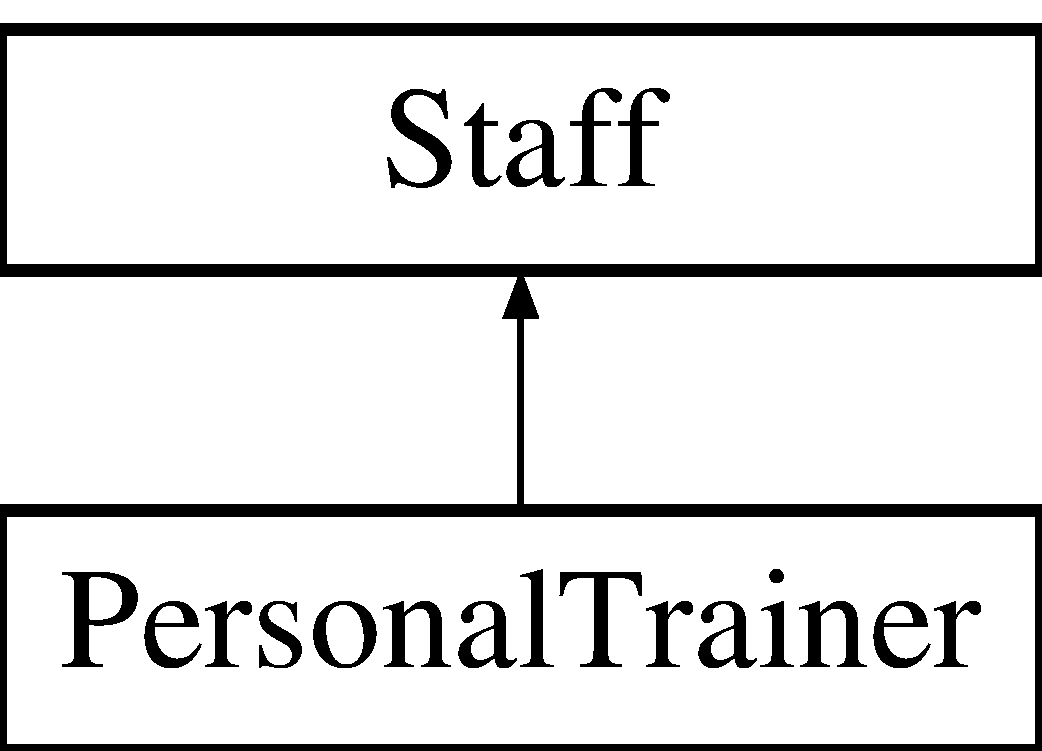
\includegraphics[height=2.000000cm]{classPersonalTrainer}
\end{center}
\end{figure}
\subsection*{Public Member Functions}
\begin{DoxyCompactItemize}
\item 
\hyperlink{classPersonalTrainer_ae327bfc36d13d337e1b4b8771f91fe1a}{Personal\+Trainer} (int \hyperlink{classStaff_ab36cd34fc6aa9c62ed9ca72263fd0ccc}{age}, double \hyperlink{classStaff_af84be4072f59d7c5c15d7c9cc07ea002}{wage}, std\+::string \hyperlink{classPersonalTrainer_aed2a4e21367c2cdd67aecba26924e17c}{specialized\+Area})
\item 
\hyperlink{classPersonalTrainer_a650aa788b90d10003feaf69e0d948fdf}{Personal\+Trainer} (std\+::string \hyperlink{classStaff_ad0e56a6c5296a2138aed86dc0cf476cb}{name}, int \hyperlink{classStaff_ab36cd34fc6aa9c62ed9ca72263fd0ccc}{age}, double \hyperlink{classStaff_af84be4072f59d7c5c15d7c9cc07ea002}{wage}, std\+::string pwd, std\+::string \hyperlink{classPersonalTrainer_aed2a4e21367c2cdd67aecba26924e17c}{specialized\+Area})
\item 
\hyperlink{classPersonalTrainer_ad3604f25652db9ee06b6bcd5c7790de6}{Personal\+Trainer} (int \hyperlink{classStaff_a2b5674cabb4b4e3a50cd130898d00c20}{id}, std\+::string \hyperlink{classStaff_ad0e56a6c5296a2138aed86dc0cf476cb}{name}, int \hyperlink{classStaff_ab36cd34fc6aa9c62ed9ca72263fd0ccc}{age}, double \hyperlink{classStaff_af84be4072f59d7c5c15d7c9cc07ea002}{wage}, std\+::string pwd, std\+::string \hyperlink{classPersonalTrainer_aed2a4e21367c2cdd67aecba26924e17c}{specialized\+Area})
\item 
virtual \hyperlink{classPersonalTrainer_ac6168e15ba23da6fae865ed923967fdd}{$\sim$\+Personal\+Trainer} ()
\item 
std\+::vector$<$ \hyperlink{classClient}{Client} $\ast$ $>$ \hyperlink{classPersonalTrainer_ad2f3a57cc4caabc6a1111f32615708a4}{get\+Clients} () const 
\item 
std\+::string \hyperlink{classPersonalTrainer_af83723e922ded3048beb9a9b3c329520}{get\+Specialized\+Area} () const 
\item 
void \hyperlink{classPersonalTrainer_a85af429825b072bbde67be03c47f604e}{set\+Schedule} (\hyperlink{classSchedule}{Schedule} \hyperlink{classStaff_ac2864b27c3cf1383c39916077b64b229}{work\+Schedule})
\item 
void \hyperlink{classPersonalTrainer_aef8f15c84017844ae7e2f38d072b9623}{set\+Clients} (std\+::vector$<$ \hyperlink{classClient}{Client} $\ast$ $>$ \hyperlink{classPersonalTrainer_a6317476679a0c3365fb02632f1af2aae}{clients})
\item 
void \hyperlink{classPersonalTrainer_a7f8580328de18489552e4f7a27448a49}{set\+Specialized\+Area} (std\+::string area)
\item 
void \hyperlink{classPersonalTrainer_a75733204b857d08f9c7db9acb5e812fc}{edit\+Personal\+Trainer} (\hyperlink{classGym}{Gym} \&gym)
\item 
void \hyperlink{classPersonalTrainer_ae864eec9478e62edc4bffea129786ea1}{edit\+Associated\+Clients} (\hyperlink{classGym}{Gym} \&gym)
\item 
virtual bool \hyperlink{classPersonalTrainer_a04c0c022242027e043c6ca355f145bba}{recognize\+Prof} () const 
\item 
void \hyperlink{classPersonalTrainer_a8dd995b0f78e00400fd0b859e90dea77}{print\+Info} ()
\end{DoxyCompactItemize}
\subsection*{Private Attributes}
\begin{DoxyCompactItemize}
\item 
std\+::vector$<$ \hyperlink{classClient}{Client} $\ast$ $>$ \hyperlink{classPersonalTrainer_a6317476679a0c3365fb02632f1af2aae}{clients}
\item 
std\+::string \hyperlink{classPersonalTrainer_aed2a4e21367c2cdd67aecba26924e17c}{specialized\+Area}
\end{DoxyCompactItemize}
\subsection*{Friends}
\begin{DoxyCompactItemize}
\item 
std\+::ostream \& \hyperlink{classPersonalTrainer_ad38066170f386e04ebc03724b00ee276}{operator$<$$<$} (std\+::ostream \&out, const \hyperlink{classPersonalTrainer}{Personal\+Trainer} \&staff)
\end{DoxyCompactItemize}


\subsection{Constructor \& Destructor Documentation}
\index{Personal\+Trainer@{Personal\+Trainer}!Personal\+Trainer@{Personal\+Trainer}}
\index{Personal\+Trainer@{Personal\+Trainer}!Personal\+Trainer@{Personal\+Trainer}}
\subsubsection[{\texorpdfstring{Personal\+Trainer(int age, double wage, std\+::string specialized\+Area)}{PersonalTrainer(int age, double wage, std::string specializedArea)}}]{\setlength{\rightskip}{0pt plus 5cm}Personal\+Trainer\+::\+Personal\+Trainer (
\begin{DoxyParamCaption}
\item[{int}]{age, }
\item[{double}]{wage, }
\item[{std\+::string}]{specialized\+Area}
\end{DoxyParamCaption}
)}\hypertarget{classPersonalTrainer_ae327bfc36d13d337e1b4b8771f91fe1a}{}\label{classPersonalTrainer_ae327bfc36d13d337e1b4b8771f91fe1a}
\index{Personal\+Trainer@{Personal\+Trainer}!Personal\+Trainer@{Personal\+Trainer}}
\index{Personal\+Trainer@{Personal\+Trainer}!Personal\+Trainer@{Personal\+Trainer}}
\subsubsection[{\texorpdfstring{Personal\+Trainer(std\+::string name, int age, double wage, std\+::string pwd, std\+::string specialized\+Area)}{PersonalTrainer(std::string name, int age, double wage, std::string pwd, std::string specializedArea)}}]{\setlength{\rightskip}{0pt plus 5cm}Personal\+Trainer\+::\+Personal\+Trainer (
\begin{DoxyParamCaption}
\item[{std\+::string}]{name, }
\item[{int}]{age, }
\item[{double}]{wage, }
\item[{std\+::string}]{pwd, }
\item[{std\+::string}]{specialized\+Area}
\end{DoxyParamCaption}
)}\hypertarget{classPersonalTrainer_a650aa788b90d10003feaf69e0d948fdf}{}\label{classPersonalTrainer_a650aa788b90d10003feaf69e0d948fdf}
\index{Personal\+Trainer@{Personal\+Trainer}!Personal\+Trainer@{Personal\+Trainer}}
\index{Personal\+Trainer@{Personal\+Trainer}!Personal\+Trainer@{Personal\+Trainer}}
\subsubsection[{\texorpdfstring{Personal\+Trainer(int id, std\+::string name, int age, double wage, std\+::string pwd, std\+::string specialized\+Area)}{PersonalTrainer(int id, std::string name, int age, double wage, std::string pwd, std::string specializedArea)}}]{\setlength{\rightskip}{0pt plus 5cm}Personal\+Trainer\+::\+Personal\+Trainer (
\begin{DoxyParamCaption}
\item[{int}]{id, }
\item[{std\+::string}]{name, }
\item[{int}]{age, }
\item[{double}]{wage, }
\item[{std\+::string}]{pwd, }
\item[{std\+::string}]{specialized\+Area}
\end{DoxyParamCaption}
)}\hypertarget{classPersonalTrainer_ad3604f25652db9ee06b6bcd5c7790de6}{}\label{classPersonalTrainer_ad3604f25652db9ee06b6bcd5c7790de6}
\index{Personal\+Trainer@{Personal\+Trainer}!````~Personal\+Trainer@{$\sim$\+Personal\+Trainer}}
\index{````~Personal\+Trainer@{$\sim$\+Personal\+Trainer}!Personal\+Trainer@{Personal\+Trainer}}
\subsubsection[{\texorpdfstring{$\sim$\+Personal\+Trainer()}{~PersonalTrainer()}}]{\setlength{\rightskip}{0pt plus 5cm}Personal\+Trainer\+::$\sim$\+Personal\+Trainer (
\begin{DoxyParamCaption}
{}
\end{DoxyParamCaption}
)\hspace{0.3cm}{\ttfamily [virtual]}}\hypertarget{classPersonalTrainer_ac6168e15ba23da6fae865ed923967fdd}{}\label{classPersonalTrainer_ac6168e15ba23da6fae865ed923967fdd}


\subsection{Member Function Documentation}
\index{Personal\+Trainer@{Personal\+Trainer}!edit\+Associated\+Clients@{edit\+Associated\+Clients}}
\index{edit\+Associated\+Clients@{edit\+Associated\+Clients}!Personal\+Trainer@{Personal\+Trainer}}
\subsubsection[{\texorpdfstring{edit\+Associated\+Clients(\+Gym \&gym)}{editAssociatedClients(Gym &gym)}}]{\setlength{\rightskip}{0pt plus 5cm}void Personal\+Trainer\+::edit\+Associated\+Clients (
\begin{DoxyParamCaption}
\item[{{\bf Gym} \&}]{gym}
\end{DoxyParamCaption}
)}\hypertarget{classPersonalTrainer_ae864eec9478e62edc4bffea129786ea1}{}\label{classPersonalTrainer_ae864eec9478e62edc4bffea129786ea1}
Handles the editing of the personal trainer\textquotesingle{}s associated clients \index{Personal\+Trainer@{Personal\+Trainer}!edit\+Personal\+Trainer@{edit\+Personal\+Trainer}}
\index{edit\+Personal\+Trainer@{edit\+Personal\+Trainer}!Personal\+Trainer@{Personal\+Trainer}}
\subsubsection[{\texorpdfstring{edit\+Personal\+Trainer(\+Gym \&gym)}{editPersonalTrainer(Gym &gym)}}]{\setlength{\rightskip}{0pt plus 5cm}void Personal\+Trainer\+::edit\+Personal\+Trainer (
\begin{DoxyParamCaption}
\item[{{\bf Gym} \&}]{gym}
\end{DoxyParamCaption}
)}\hypertarget{classPersonalTrainer_a75733204b857d08f9c7db9acb5e812fc}{}\label{classPersonalTrainer_a75733204b857d08f9c7db9acb5e812fc}
Handles the editing of the personal trainer\textquotesingle{}s information \index{Personal\+Trainer@{Personal\+Trainer}!get\+Clients@{get\+Clients}}
\index{get\+Clients@{get\+Clients}!Personal\+Trainer@{Personal\+Trainer}}
\subsubsection[{\texorpdfstring{get\+Clients() const }{getClients() const }}]{\setlength{\rightskip}{0pt plus 5cm}vector$<$ {\bf Client} $\ast$ $>$ Personal\+Trainer\+::get\+Clients (
\begin{DoxyParamCaption}
{}
\end{DoxyParamCaption}
) const}\hypertarget{classPersonalTrainer_ad2f3a57cc4caabc6a1111f32615708a4}{}\label{classPersonalTrainer_ad2f3a57cc4caabc6a1111f32615708a4}
Returns the vector of clients of the personal trainer

\begin{DoxyReturn}{Returns}
Returns vector of pointers to clients of the personal trainer 
\end{DoxyReturn}
\index{Personal\+Trainer@{Personal\+Trainer}!get\+Specialized\+Area@{get\+Specialized\+Area}}
\index{get\+Specialized\+Area@{get\+Specialized\+Area}!Personal\+Trainer@{Personal\+Trainer}}
\subsubsection[{\texorpdfstring{get\+Specialized\+Area() const }{getSpecializedArea() const }}]{\setlength{\rightskip}{0pt plus 5cm}string Personal\+Trainer\+::get\+Specialized\+Area (
\begin{DoxyParamCaption}
{}
\end{DoxyParamCaption}
) const}\hypertarget{classPersonalTrainer_af83723e922ded3048beb9a9b3c329520}{}\label{classPersonalTrainer_af83723e922ded3048beb9a9b3c329520}
Returns the specialized area of the personal trainer

\begin{DoxyReturn}{Returns}
Returns the specialized area as a string 
\end{DoxyReturn}
\index{Personal\+Trainer@{Personal\+Trainer}!print\+Info@{print\+Info}}
\index{print\+Info@{print\+Info}!Personal\+Trainer@{Personal\+Trainer}}
\subsubsection[{\texorpdfstring{print\+Info()}{printInfo()}}]{\setlength{\rightskip}{0pt plus 5cm}void Personal\+Trainer\+::print\+Info (
\begin{DoxyParamCaption}
{}
\end{DoxyParamCaption}
)\hspace{0.3cm}{\ttfamily [virtual]}}\hypertarget{classPersonalTrainer_a8dd995b0f78e00400fd0b859e90dea77}{}\label{classPersonalTrainer_a8dd995b0f78e00400fd0b859e90dea77}
Displays information about Personal Trainer 
\begin{DoxyParams}{Parameters}
{\em } & \\
\hline
\end{DoxyParams}


Reimplemented from \hyperlink{classStaff_a64b23946e927025bf5aec2938502305a}{Staff}.

\index{Personal\+Trainer@{Personal\+Trainer}!recognize\+Prof@{recognize\+Prof}}
\index{recognize\+Prof@{recognize\+Prof}!Personal\+Trainer@{Personal\+Trainer}}
\subsubsection[{\texorpdfstring{recognize\+Prof() const }{recognizeProf() const }}]{\setlength{\rightskip}{0pt plus 5cm}bool Personal\+Trainer\+::recognize\+Prof (
\begin{DoxyParamCaption}
{}
\end{DoxyParamCaption}
) const\hspace{0.3cm}{\ttfamily [virtual]}}\hypertarget{classPersonalTrainer_a04c0c022242027e043c6ca355f145bba}{}\label{classPersonalTrainer_a04c0c022242027e043c6ca355f145bba}


Reimplemented from \hyperlink{classStaff_a3c0c4690bacca349c84f707004c3acb0}{Staff}.

\index{Personal\+Trainer@{Personal\+Trainer}!set\+Clients@{set\+Clients}}
\index{set\+Clients@{set\+Clients}!Personal\+Trainer@{Personal\+Trainer}}
\subsubsection[{\texorpdfstring{set\+Clients(std\+::vector$<$ Client $\ast$ $>$ clients)}{setClients(std::vector< Client * > clients)}}]{\setlength{\rightskip}{0pt plus 5cm}void Personal\+Trainer\+::set\+Clients (
\begin{DoxyParamCaption}
\item[{std\+::vector$<$ {\bf Client} $\ast$ $>$}]{clients}
\end{DoxyParamCaption}
)}\hypertarget{classPersonalTrainer_aef8f15c84017844ae7e2f38d072b9623}{}\label{classPersonalTrainer_aef8f15c84017844ae7e2f38d072b9623}
Sets the clients of the personal trainer


\begin{DoxyParams}{Parameters}
{\em Vector} & of pointers to clients \\
\hline
\end{DoxyParams}
\index{Personal\+Trainer@{Personal\+Trainer}!set\+Schedule@{set\+Schedule}}
\index{set\+Schedule@{set\+Schedule}!Personal\+Trainer@{Personal\+Trainer}}
\subsubsection[{\texorpdfstring{set\+Schedule(\+Schedule work\+Schedule)}{setSchedule(Schedule workSchedule)}}]{\setlength{\rightskip}{0pt plus 5cm}void Personal\+Trainer\+::set\+Schedule (
\begin{DoxyParamCaption}
\item[{{\bf Schedule}}]{work\+Schedule}
\end{DoxyParamCaption}
)}\hypertarget{classPersonalTrainer_a85af429825b072bbde67be03c47f604e}{}\label{classPersonalTrainer_a85af429825b072bbde67be03c47f604e}
Sets the working schedule of the personal trainer 
\begin{DoxyParams}{Parameters}
{\em The} & working schedule of the personal trainer \\
\hline
\end{DoxyParams}
\index{Personal\+Trainer@{Personal\+Trainer}!set\+Specialized\+Area@{set\+Specialized\+Area}}
\index{set\+Specialized\+Area@{set\+Specialized\+Area}!Personal\+Trainer@{Personal\+Trainer}}
\subsubsection[{\texorpdfstring{set\+Specialized\+Area(std\+::string area)}{setSpecializedArea(std::string area)}}]{\setlength{\rightskip}{0pt plus 5cm}void Personal\+Trainer\+::set\+Specialized\+Area (
\begin{DoxyParamCaption}
\item[{std\+::string}]{area}
\end{DoxyParamCaption}
)}\hypertarget{classPersonalTrainer_a7f8580328de18489552e4f7a27448a49}{}\label{classPersonalTrainer_a7f8580328de18489552e4f7a27448a49}
Sets the specialized area of the personal trainer


\begin{DoxyParams}{Parameters}
{\em The} & specialized area of the personal trainer \\
\hline
\end{DoxyParams}


\subsection{Friends And Related Function Documentation}
\index{Personal\+Trainer@{Personal\+Trainer}!operator$<$$<$@{operator$<$$<$}}
\index{operator$<$$<$@{operator$<$$<$}!Personal\+Trainer@{Personal\+Trainer}}
\subsubsection[{\texorpdfstring{operator$<$$<$}{operator<<}}]{\setlength{\rightskip}{0pt plus 5cm}std\+::ostream\& operator$<$$<$ (
\begin{DoxyParamCaption}
\item[{std\+::ostream \&}]{out, }
\item[{const {\bf Personal\+Trainer} \&}]{staff}
\end{DoxyParamCaption}
)\hspace{0.3cm}{\ttfamily [friend]}}\hypertarget{classPersonalTrainer_ad38066170f386e04ebc03724b00ee276}{}\label{classPersonalTrainer_ad38066170f386e04ebc03724b00ee276}
Overload of operator $<$$<$ for derived class Personal Trainer \begin{DoxyReturn}{Returns}
ostream 
\end{DoxyReturn}


\subsection{Member Data Documentation}
\index{Personal\+Trainer@{Personal\+Trainer}!clients@{clients}}
\index{clients@{clients}!Personal\+Trainer@{Personal\+Trainer}}
\subsubsection[{\texorpdfstring{clients}{clients}}]{\setlength{\rightskip}{0pt plus 5cm}std\+::vector$<${\bf Client} $\ast$$>$ Personal\+Trainer\+::clients\hspace{0.3cm}{\ttfamily [private]}}\hypertarget{classPersonalTrainer_a6317476679a0c3365fb02632f1af2aae}{}\label{classPersonalTrainer_a6317476679a0c3365fb02632f1af2aae}
\index{Personal\+Trainer@{Personal\+Trainer}!specialized\+Area@{specialized\+Area}}
\index{specialized\+Area@{specialized\+Area}!Personal\+Trainer@{Personal\+Trainer}}
\subsubsection[{\texorpdfstring{specialized\+Area}{specializedArea}}]{\setlength{\rightskip}{0pt plus 5cm}std\+::string Personal\+Trainer\+::specialized\+Area\hspace{0.3cm}{\ttfamily [private]}}\hypertarget{classPersonalTrainer_aed2a4e21367c2cdd67aecba26924e17c}{}\label{classPersonalTrainer_aed2a4e21367c2cdd67aecba26924e17c}


The documentation for this class was generated from the following files\+:\begin{DoxyCompactItemize}
\item 
\hyperlink{PersonalTrainer_8h}{Personal\+Trainer.\+h}\item 
\hyperlink{PersonalTrainer_8cpp}{Personal\+Trainer.\+cpp}\end{DoxyCompactItemize}

\hypertarget{classProgram}{}\section{Program Class Reference}
\label{classProgram}\index{Program@{Program}}


{\ttfamily \#include $<$Program.\+h$>$}

\subsection*{Public Member Functions}
\begin{DoxyCompactItemize}
\item 
\hyperlink{classProgram_a77354e42fdc0bc2e020aa1ea43204838}{Program} (int \hyperlink{classProgram_a95ee4089c38ba823287d4d9a4057cff4}{code})
\item 
\hyperlink{classProgram_a2ec985383c63de0819b0fa45ed924d8d}{Program} (int \hyperlink{classProgram_a95ee4089c38ba823287d4d9a4057cff4}{code}, int \hyperlink{classProgram_a3b0559f1f16d662f885851113a31a3a6}{days}, float \hyperlink{classProgram_a59057576469cca4e1b012010af18538c}{cost})
\item 
\hyperlink{classProgram_a986aef1c50e1d338a3315a47ba6df549}{$\sim$\+Program} ()
\item 
int \hyperlink{classProgram_a6ad5b040a2b51e7aaec0c0dfa06df151}{get\+Days} () const 
\item 
float \hyperlink{classProgram_a50fdcb0e6e8389a98d80e51f85e016e8}{get\+Cost} () const 
\item 
int \hyperlink{classProgram_aa6b4bdc285eb9b8461b6bb1b7319dcc7}{get\+Code} () const 
\item 
void \hyperlink{classProgram_ab80d635627245152d90a8be1857d0cb9}{set\+Days} (int \hyperlink{classProgram_a3b0559f1f16d662f885851113a31a3a6}{days})
\item 
void \hyperlink{classProgram_a22a51b02ac6c4c880a3d932d1d987bd5}{set\+Cost} (float \hyperlink{classProgram_a59057576469cca4e1b012010af18538c}{cost})
\item 
void \hyperlink{classProgram_acae5e9997c86dca01f4f2f08b7fbed83}{set\+Code} (int \hyperlink{classProgram_a95ee4089c38ba823287d4d9a4057cff4}{code})
\item 
void \hyperlink{classProgram_aabc3da82094e4879cee242dd5cc2ad0f}{edit\+Program} (\hyperlink{classGym}{Gym} \&gym)
\end{DoxyCompactItemize}
\subsection*{Private Attributes}
\begin{DoxyCompactItemize}
\item 
int \hyperlink{classProgram_a95ee4089c38ba823287d4d9a4057cff4}{code}
\item 
int \hyperlink{classProgram_a3b0559f1f16d662f885851113a31a3a6}{days}
\item 
float \hyperlink{classProgram_a59057576469cca4e1b012010af18538c}{cost}
\end{DoxyCompactItemize}
\subsection*{Friends}
\begin{DoxyCompactItemize}
\item 
std\+::ostream \& \hyperlink{classProgram_a328f4c8ee5e4b87028767f36a1cbf1a6}{operator$<$$<$} (std\+::ostream \&out, const \hyperlink{classProgram}{Program} \&program)
\end{DoxyCompactItemize}


\subsection{Constructor \& Destructor Documentation}
\index{Program@{Program}!Program@{Program}}
\index{Program@{Program}!Program@{Program}}
\subsubsection[{\texorpdfstring{Program(int code)}{Program(int code)}}]{\setlength{\rightskip}{0pt plus 5cm}Program\+::\+Program (
\begin{DoxyParamCaption}
\item[{int}]{code}
\end{DoxyParamCaption}
)}\hypertarget{classProgram_a77354e42fdc0bc2e020aa1ea43204838}{}\label{classProgram_a77354e42fdc0bc2e020aa1ea43204838}
\index{Program@{Program}!Program@{Program}}
\index{Program@{Program}!Program@{Program}}
\subsubsection[{\texorpdfstring{Program(int code, int days, float cost)}{Program(int code, int days, float cost)}}]{\setlength{\rightskip}{0pt plus 5cm}Program\+::\+Program (
\begin{DoxyParamCaption}
\item[{int}]{code, }
\item[{int}]{days, }
\item[{float}]{cost}
\end{DoxyParamCaption}
)}\hypertarget{classProgram_a2ec985383c63de0819b0fa45ed924d8d}{}\label{classProgram_a2ec985383c63de0819b0fa45ed924d8d}
\index{Program@{Program}!````~Program@{$\sim$\+Program}}
\index{````~Program@{$\sim$\+Program}!Program@{Program}}
\subsubsection[{\texorpdfstring{$\sim$\+Program()}{~Program()}}]{\setlength{\rightskip}{0pt plus 5cm}Program\+::$\sim$\+Program (
\begin{DoxyParamCaption}
{}
\end{DoxyParamCaption}
)}\hypertarget{classProgram_a986aef1c50e1d338a3315a47ba6df549}{}\label{classProgram_a986aef1c50e1d338a3315a47ba6df549}


\subsection{Member Function Documentation}
\index{Program@{Program}!edit\+Program@{edit\+Program}}
\index{edit\+Program@{edit\+Program}!Program@{Program}}
\subsubsection[{\texorpdfstring{edit\+Program(\+Gym \&gym)}{editProgram(Gym &gym)}}]{\setlength{\rightskip}{0pt plus 5cm}void Program\+::edit\+Program (
\begin{DoxyParamCaption}
\item[{{\bf Gym} \&}]{gym}
\end{DoxyParamCaption}
)}\hypertarget{classProgram_aabc3da82094e4879cee242dd5cc2ad0f}{}\label{classProgram_aabc3da82094e4879cee242dd5cc2ad0f}
Edits program\textquotesingle{}s information \index{Program@{Program}!get\+Code@{get\+Code}}
\index{get\+Code@{get\+Code}!Program@{Program}}
\subsubsection[{\texorpdfstring{get\+Code() const }{getCode() const }}]{\setlength{\rightskip}{0pt plus 5cm}int Program\+::get\+Code (
\begin{DoxyParamCaption}
{}
\end{DoxyParamCaption}
) const}\hypertarget{classProgram_aa6b4bdc285eb9b8461b6bb1b7319dcc7}{}\label{classProgram_aa6b4bdc285eb9b8461b6bb1b7319dcc7}
Returns the code of the \hyperlink{classProgram}{Program}


\begin{DoxyParams}{Parameters}
{\em } & \\
\hline
\end{DoxyParams}
\index{Program@{Program}!get\+Cost@{get\+Cost}}
\index{get\+Cost@{get\+Cost}!Program@{Program}}
\subsubsection[{\texorpdfstring{get\+Cost() const }{getCost() const }}]{\setlength{\rightskip}{0pt plus 5cm}float Program\+::get\+Cost (
\begin{DoxyParamCaption}
{}
\end{DoxyParamCaption}
) const}\hypertarget{classProgram_a50fdcb0e6e8389a98d80e51f85e016e8}{}\label{classProgram_a50fdcb0e6e8389a98d80e51f85e016e8}
Returns the cost of the \hyperlink{classProgram}{Program}


\begin{DoxyParams}{Parameters}
{\em } & \\
\hline
\end{DoxyParams}
\index{Program@{Program}!get\+Days@{get\+Days}}
\index{get\+Days@{get\+Days}!Program@{Program}}
\subsubsection[{\texorpdfstring{get\+Days() const }{getDays() const }}]{\setlength{\rightskip}{0pt plus 5cm}int Program\+::get\+Days (
\begin{DoxyParamCaption}
{}
\end{DoxyParamCaption}
) const}\hypertarget{classProgram_a6ad5b040a2b51e7aaec0c0dfa06df151}{}\label{classProgram_a6ad5b040a2b51e7aaec0c0dfa06df151}
Returns the number of days a the \hyperlink{classProgram}{Program} gives


\begin{DoxyParams}{Parameters}
{\em } & \\
\hline
\end{DoxyParams}
\index{Program@{Program}!set\+Code@{set\+Code}}
\index{set\+Code@{set\+Code}!Program@{Program}}
\subsubsection[{\texorpdfstring{set\+Code(int code)}{setCode(int code)}}]{\setlength{\rightskip}{0pt plus 5cm}void Program\+::set\+Code (
\begin{DoxyParamCaption}
\item[{int}]{code}
\end{DoxyParamCaption}
)}\hypertarget{classProgram_acae5e9997c86dca01f4f2f08b7fbed83}{}\label{classProgram_acae5e9997c86dca01f4f2f08b7fbed83}
Sets program\textquotesingle{}s code


\begin{DoxyParams}{Parameters}
{\em program\textquotesingle{}s} & code \\
\hline
\end{DoxyParams}
\index{Program@{Program}!set\+Cost@{set\+Cost}}
\index{set\+Cost@{set\+Cost}!Program@{Program}}
\subsubsection[{\texorpdfstring{set\+Cost(float cost)}{setCost(float cost)}}]{\setlength{\rightskip}{0pt plus 5cm}void Program\+::set\+Cost (
\begin{DoxyParamCaption}
\item[{float}]{cost}
\end{DoxyParamCaption}
)}\hypertarget{classProgram_a22a51b02ac6c4c880a3d932d1d987bd5}{}\label{classProgram_a22a51b02ac6c4c880a3d932d1d987bd5}
Sets cost of program


\begin{DoxyParams}{Parameters}
{\em program\textquotesingle{}s} & cost \\
\hline
\end{DoxyParams}
\index{Program@{Program}!set\+Days@{set\+Days}}
\index{set\+Days@{set\+Days}!Program@{Program}}
\subsubsection[{\texorpdfstring{set\+Days(int days)}{setDays(int days)}}]{\setlength{\rightskip}{0pt plus 5cm}void Program\+::set\+Days (
\begin{DoxyParamCaption}
\item[{int}]{days}
\end{DoxyParamCaption}
)}\hypertarget{classProgram_ab80d635627245152d90a8be1857d0cb9}{}\label{classProgram_ab80d635627245152d90a8be1857d0cb9}
Sets number of program\textquotesingle{}s gym days


\begin{DoxyParams}{Parameters}
{\em number} & of program\textquotesingle{}s gym days \\
\hline
\end{DoxyParams}


\subsection{Friends And Related Function Documentation}
\index{Program@{Program}!operator$<$$<$@{operator$<$$<$}}
\index{operator$<$$<$@{operator$<$$<$}!Program@{Program}}
\subsubsection[{\texorpdfstring{operator$<$$<$}{operator<<}}]{\setlength{\rightskip}{0pt plus 5cm}std\+::ostream\& operator$<$$<$ (
\begin{DoxyParamCaption}
\item[{std\+::ostream \&}]{out, }
\item[{const {\bf Program} \&}]{program}
\end{DoxyParamCaption}
)\hspace{0.3cm}{\ttfamily [friend]}}\hypertarget{classProgram_a328f4c8ee5e4b87028767f36a1cbf1a6}{}\label{classProgram_a328f4c8ee5e4b87028767f36a1cbf1a6}
Prints the \hyperlink{classProgram}{Program} information 

\subsection{Member Data Documentation}
\index{Program@{Program}!code@{code}}
\index{code@{code}!Program@{Program}}
\subsubsection[{\texorpdfstring{code}{code}}]{\setlength{\rightskip}{0pt plus 5cm}int Program\+::code\hspace{0.3cm}{\ttfamily [private]}}\hypertarget{classProgram_a95ee4089c38ba823287d4d9a4057cff4}{}\label{classProgram_a95ee4089c38ba823287d4d9a4057cff4}
\index{Program@{Program}!cost@{cost}}
\index{cost@{cost}!Program@{Program}}
\subsubsection[{\texorpdfstring{cost}{cost}}]{\setlength{\rightskip}{0pt plus 5cm}float Program\+::cost\hspace{0.3cm}{\ttfamily [private]}}\hypertarget{classProgram_a59057576469cca4e1b012010af18538c}{}\label{classProgram_a59057576469cca4e1b012010af18538c}
\index{Program@{Program}!days@{days}}
\index{days@{days}!Program@{Program}}
\subsubsection[{\texorpdfstring{days}{days}}]{\setlength{\rightskip}{0pt plus 5cm}int Program\+::days\hspace{0.3cm}{\ttfamily [private]}}\hypertarget{classProgram_a3b0559f1f16d662f885851113a31a3a6}{}\label{classProgram_a3b0559f1f16d662f885851113a31a3a6}


The documentation for this class was generated from the following files\+:\begin{DoxyCompactItemize}
\item 
\hyperlink{Program_8h}{Program.\+h}\item 
\hyperlink{Program_8cpp}{Program.\+cpp}\end{DoxyCompactItemize}

\hypertarget{classSchedule}{}\section{Schedule Class Reference}
\label{classSchedule}\index{Schedule@{Schedule}}


{\ttfamily \#include $<$Schedule.\+h$>$}

\subsection*{Public Member Functions}
\begin{DoxyCompactItemize}
\item 
\hyperlink{classSchedule_a878716f4043a016224a14f78974edf1d}{Schedule} ()
\item 
virtual \hyperlink{classSchedule_a4806b985197d35c00b9e707c0ed87998}{$\sim$\+Schedule} ()
\item 
bool \hyperlink{classSchedule_ad7f876b27af5e115dd8dcfa2444a2897}{add\+Date} (const \hyperlink{classDate}{Date} \&date\+Start, const \hyperlink{classDate}{Date} \&date\+Finish)
\begin{DoxyCompactList}\small\item\em Add a date to the schedule. \end{DoxyCompactList}\item 
std\+::set$<$ std\+::pair$<$ \hyperlink{classDate}{Date}, \hyperlink{classDate}{Date} $>$ $\ast$, \hyperlink{structAPtrComp}{A\+Ptr\+Comp} $>$ \hyperlink{classSchedule_a8e7f2e6ddf3671f50d0c7393b5a76f13}{get\+Schedule\+Set} ()
\begin{DoxyCompactList}\small\item\em Returns the schr. \end{DoxyCompactList}\end{DoxyCompactItemize}
\subsection*{Private Attributes}
\begin{DoxyCompactItemize}
\item 
std\+::set$<$ std\+::pair$<$ \hyperlink{classDate}{Date}, \hyperlink{classDate}{Date} $>$ $\ast$, \hyperlink{structAPtrComp}{A\+Ptr\+Comp} $>$ \hyperlink{classSchedule_a1774807b89cc782ba1a3bafc93b1fb70}{schedule}
\end{DoxyCompactItemize}
\subsection*{Friends}
\begin{DoxyCompactItemize}
\item 
std\+::ostream \& \hyperlink{classSchedule_a601593037b72868ce945f1302d2a3b42}{operator$<$$<$} (std\+::ostream \&out, const \hyperlink{classSchedule}{Schedule} \&\hyperlink{classSchedule_a1774807b89cc782ba1a3bafc93b1fb70}{schedule})
\begin{DoxyCompactList}\small\item\em Prints in a user-\/friendly way the schedule. \end{DoxyCompactList}\end{DoxyCompactItemize}


\subsection{Constructor \& Destructor Documentation}
\index{Schedule@{Schedule}!Schedule@{Schedule}}
\index{Schedule@{Schedule}!Schedule@{Schedule}}
\subsubsection[{\texorpdfstring{Schedule()}{Schedule()}}]{\setlength{\rightskip}{0pt plus 5cm}Schedule\+::\+Schedule (
\begin{DoxyParamCaption}
{}
\end{DoxyParamCaption}
)}\hypertarget{classSchedule_a878716f4043a016224a14f78974edf1d}{}\label{classSchedule_a878716f4043a016224a14f78974edf1d}
\index{Schedule@{Schedule}!````~Schedule@{$\sim$\+Schedule}}
\index{````~Schedule@{$\sim$\+Schedule}!Schedule@{Schedule}}
\subsubsection[{\texorpdfstring{$\sim$\+Schedule()}{~Schedule()}}]{\setlength{\rightskip}{0pt plus 5cm}Schedule\+::$\sim$\+Schedule (
\begin{DoxyParamCaption}
{}
\end{DoxyParamCaption}
)\hspace{0.3cm}{\ttfamily [virtual]}}\hypertarget{classSchedule_a4806b985197d35c00b9e707c0ed87998}{}\label{classSchedule_a4806b985197d35c00b9e707c0ed87998}


\subsection{Member Function Documentation}
\index{Schedule@{Schedule}!add\+Date@{add\+Date}}
\index{add\+Date@{add\+Date}!Schedule@{Schedule}}
\subsubsection[{\texorpdfstring{add\+Date(const Date \&date\+Start, const Date \&date\+Finish)}{addDate(const Date &dateStart, const Date &dateFinish)}}]{\setlength{\rightskip}{0pt plus 5cm}bool Schedule\+::add\+Date (
\begin{DoxyParamCaption}
\item[{const {\bf Date} \&}]{date\+Start, }
\item[{const {\bf Date} \&}]{date\+Finish}
\end{DoxyParamCaption}
)}\hypertarget{classSchedule_ad7f876b27af5e115dd8dcfa2444a2897}{}\label{classSchedule_ad7f876b27af5e115dd8dcfa2444a2897}


Add a date to the schedule. 


\begin{DoxyParams}{Parameters}
{\em date\+Start} & Time interval start date \\
\hline
{\em date\+Start} & Time interval finish date\\
\hline
\end{DoxyParams}
\begin{DoxyReturn}{Returns}
Returns true if the time interval was added successfully and returns false otherwise 
\end{DoxyReturn}
\index{Schedule@{Schedule}!get\+Schedule\+Set@{get\+Schedule\+Set}}
\index{get\+Schedule\+Set@{get\+Schedule\+Set}!Schedule@{Schedule}}
\subsubsection[{\texorpdfstring{get\+Schedule\+Set()}{getScheduleSet()}}]{\setlength{\rightskip}{0pt plus 5cm}std\+::set$<$ std\+::pair$<$ {\bf Date}, {\bf Date} $>$ $\ast$, {\bf A\+Ptr\+Comp} $>$ Schedule\+::get\+Schedule\+Set (
\begin{DoxyParamCaption}
{}
\end{DoxyParamCaption}
)}\hypertarget{classSchedule_a8e7f2e6ddf3671f50d0c7393b5a76f13}{}\label{classSchedule_a8e7f2e6ddf3671f50d0c7393b5a76f13}


Returns the schr. 


\begin{DoxyParams}{Parameters}
{\em out} & Output stream \\
\hline
{\em schedule} & \hyperlink{classSchedule}{Schedule} object\\
\hline
\end{DoxyParams}
\begin{DoxyReturn}{Returns}
The a set representing the schedule 
\end{DoxyReturn}


\subsection{Friends And Related Function Documentation}
\index{Schedule@{Schedule}!operator$<$$<$@{operator$<$$<$}}
\index{operator$<$$<$@{operator$<$$<$}!Schedule@{Schedule}}
\subsubsection[{\texorpdfstring{operator$<$$<$}{operator<<}}]{\setlength{\rightskip}{0pt plus 5cm}std\+::ostream\& operator$<$$<$ (
\begin{DoxyParamCaption}
\item[{std\+::ostream \&}]{out, }
\item[{const {\bf Schedule} \&}]{schedule}
\end{DoxyParamCaption}
)\hspace{0.3cm}{\ttfamily [friend]}}\hypertarget{classSchedule_a601593037b72868ce945f1302d2a3b42}{}\label{classSchedule_a601593037b72868ce945f1302d2a3b42}


Prints in a user-\/friendly way the schedule. 


\begin{DoxyParams}{Parameters}
{\em out} & Output stream \\
\hline
{\em schedule} & \hyperlink{classSchedule}{Schedule} object\\
\hline
\end{DoxyParams}
@ output stream 

\subsection{Member Data Documentation}
\index{Schedule@{Schedule}!schedule@{schedule}}
\index{schedule@{schedule}!Schedule@{Schedule}}
\subsubsection[{\texorpdfstring{schedule}{schedule}}]{\setlength{\rightskip}{0pt plus 5cm}std\+::set$<$std\+::pair$<${\bf Date},{\bf Date}$>$$\ast$,{\bf A\+Ptr\+Comp}$>$ Schedule\+::schedule\hspace{0.3cm}{\ttfamily [private]}}\hypertarget{classSchedule_a1774807b89cc782ba1a3bafc93b1fb70}{}\label{classSchedule_a1774807b89cc782ba1a3bafc93b1fb70}


The documentation for this class was generated from the following files\+:\begin{DoxyCompactItemize}
\item 
\hyperlink{Schedule_8h}{Schedule.\+h}\item 
\hyperlink{Schedule_8cpp}{Schedule.\+cpp}\end{DoxyCompactItemize}

\hypertarget{classStaff}{}\section{Staff Class Reference}
\label{classStaff}\index{Staff@{Staff}}


{\ttfamily \#include $<$Staff.\+h$>$}

Inheritance diagram for Staff\+:\begin{figure}[H]
\begin{center}
\leavevmode
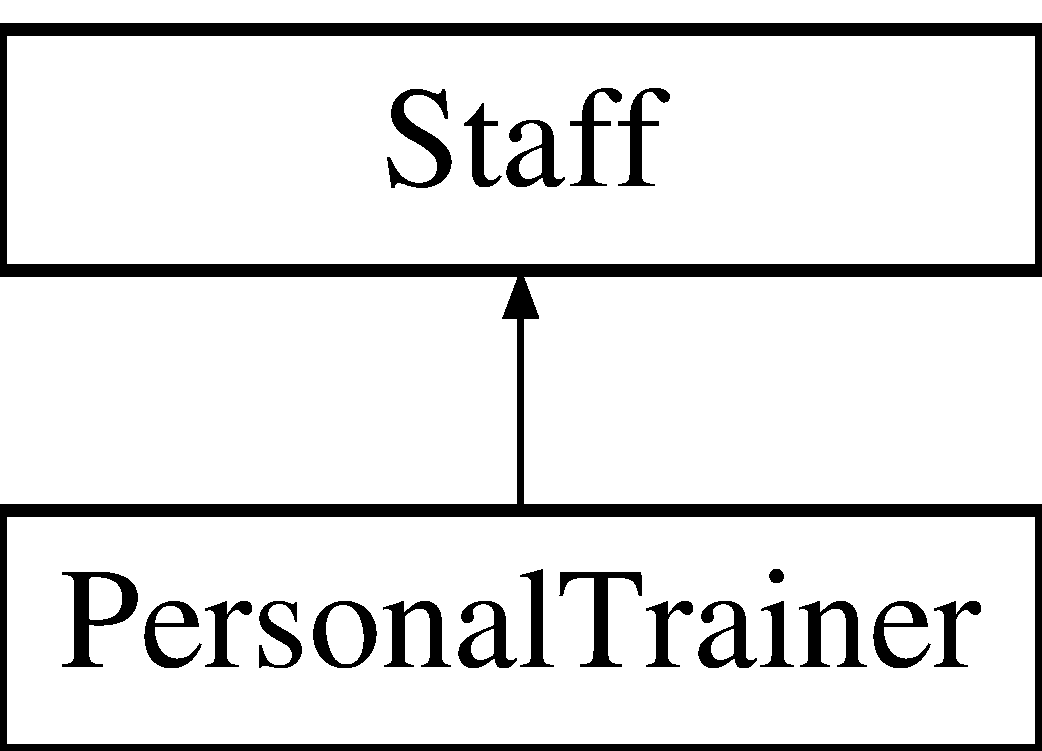
\includegraphics[height=2.000000cm]{classStaff}
\end{center}
\end{figure}
\subsection*{Public Member Functions}
\begin{DoxyCompactItemize}
\item 
\hyperlink{classStaff_a94a7d66467d3946143dd9c5fe4ef4c6c}{Staff} (int \hyperlink{classStaff_ab36cd34fc6aa9c62ed9ca72263fd0ccc}{age}, double \hyperlink{classStaff_af84be4072f59d7c5c15d7c9cc07ea002}{wage})
\item 
\hyperlink{classStaff_a0b2629c64afc440decf47e6746def943}{Staff} (std\+::string \hyperlink{classStaff_ad0e56a6c5296a2138aed86dc0cf476cb}{name}, int \hyperlink{classStaff_ab36cd34fc6aa9c62ed9ca72263fd0ccc}{age}, double \hyperlink{classStaff_af84be4072f59d7c5c15d7c9cc07ea002}{wage}, std\+::string pwd)
\item 
\hyperlink{classStaff_a7d0a5c2377512828c73f88a4f7c2213c}{Staff} (int \hyperlink{classStaff_a2b5674cabb4b4e3a50cd130898d00c20}{id}, std\+::string \hyperlink{classStaff_ad0e56a6c5296a2138aed86dc0cf476cb}{name}, int \hyperlink{classStaff_ab36cd34fc6aa9c62ed9ca72263fd0ccc}{age}, double \hyperlink{classStaff_af84be4072f59d7c5c15d7c9cc07ea002}{wage}, std\+::string pwd)
\item 
virtual \hyperlink{classStaff_a1c2f98aad2fbd5ddf72e9ff92304cbfd}{$\sim$\+Staff} ()
\item 
void \hyperlink{classStaff_a440c94e1d94a37384bc0f54f2709c083}{increment\+Staff\+Id} ()
\item 
virtual int \hyperlink{classStaff_aaad9e092c09d644570cf4119e2c77368}{get\+Id} () const 
\item 
virtual std\+::string \hyperlink{classStaff_a75431ea3462f0862f00884842cb032a1}{get\+Name} () const 
\item 
virtual int \hyperlink{classStaff_acd4f7e81f745e6a5205acbdf9b6ada2c}{get\+Age} () const 
\item 
virtual double \hyperlink{classStaff_a191d2c46bc1b5be8899e55bc0823a920}{get\+Wage} () const 
\item 
virtual bool \hyperlink{classStaff_a3c0c4690bacca349c84f707004c3acb0}{recognize\+Prof} () const 
\item 
std\+::string \hyperlink{classStaff_a6cb9453d71022d92c93e364fe51c1c0c}{get\+Password} () const 
\item 
bool \hyperlink{classStaff_a3dc1d93121a3fe8630475f29fa68823f}{is\+Inside\+Gym} () const 
\item 
bool \hyperlink{classStaff_ab23c34f9b2807218af83802461cc44d8}{get\+Was\+Paid} () const 
\item 
void \hyperlink{classStaff_a6c6eb931f55c44a1cd21994f51807c54}{set\+Name} (std\+::string \hyperlink{classStaff_ad0e56a6c5296a2138aed86dc0cf476cb}{name})
\item 
void \hyperlink{classStaff_a710ece17d20ae2de66d9ed2a550b15f1}{set\+Age} (int \hyperlink{classStaff_ab36cd34fc6aa9c62ed9ca72263fd0ccc}{age})
\item 
void \hyperlink{classStaff_aa6584dd4ddea731360eb621b03a9216b}{set\+Schedule} (\hyperlink{classSchedule}{Schedule} \hyperlink{classStaff_ac2864b27c3cf1383c39916077b64b229}{work\+Schedule})
\item 
void \hyperlink{classStaff_a0a8faa8566d285282d7eb3848ea44249}{set\+Wage} (double \hyperlink{classStaff_af84be4072f59d7c5c15d7c9cc07ea002}{wage})
\item 
void \hyperlink{classStaff_aaf97f05a90562a808af9f8215b67a758}{set\+Password} (std\+::string pass)
\item 
void \hyperlink{classStaff_a70c5d5efb82fe587a69b3fe7ef44bf30}{change\+Was\+Paid} ()
\item 
void \hyperlink{classStaff_a7dc07b6a8330a7cf0117604d7cbd5138}{change\+Location} ()
\item 
void \hyperlink{classStaff_a139297bfe1533cf2b085e812365d1b38}{edit\+Staff} (\hyperlink{classGym}{Gym} \&gym)
\item 
bool \hyperlink{classStaff_a41f6fa58ad71fcb821edfbc2b838319e}{auth} (std\+::string pass)
\item 
virtual void \hyperlink{classStaff_a64b23946e927025bf5aec2938502305a}{print\+Info} ()
\end{DoxyCompactItemize}
\subsection*{Private Attributes}
\begin{DoxyCompactItemize}
\item 
int \hyperlink{classStaff_a2b5674cabb4b4e3a50cd130898d00c20}{id}
\item 
std\+::string \hyperlink{classStaff_ad0e56a6c5296a2138aed86dc0cf476cb}{name}
\item 
int \hyperlink{classStaff_ab36cd34fc6aa9c62ed9ca72263fd0ccc}{age}
\item 
double \hyperlink{classStaff_af84be4072f59d7c5c15d7c9cc07ea002}{wage}
\item 
bool \hyperlink{classStaff_a352968c949ea47dd9a278bd2d35e1fb9}{inside\+Gym}
\item 
bool \hyperlink{classStaff_ae1f9f88528e62ba09e50966a46353208}{was\+Paid}
\item 
\hyperlink{classSchedule}{Schedule} \hyperlink{classStaff_ac2864b27c3cf1383c39916077b64b229}{work\+Schedule}
\item 
std\+::string \hyperlink{classStaff_a1500c35ca5bc4a9fedd5cfb960c9bee1}{password}
\end{DoxyCompactItemize}
\subsection*{Static Private Attributes}
\begin{DoxyCompactItemize}
\item 
static int \hyperlink{classStaff_a5eb1171ba3343325d4c999df8c29e6bf}{staff\+Id} = 0
\end{DoxyCompactItemize}
\subsection*{Friends}
\begin{DoxyCompactItemize}
\item 
std\+::ostream \& \hyperlink{classStaff_a4edf96b40bf376890c80c952bae628c6}{operator$<$$<$} (std\+::ostream \&out, const \hyperlink{classStaff}{Staff} \&staff)
\end{DoxyCompactItemize}


\subsection{Constructor \& Destructor Documentation}
\index{Staff@{Staff}!Staff@{Staff}}
\index{Staff@{Staff}!Staff@{Staff}}
\subsubsection[{\texorpdfstring{Staff(int age, double wage)}{Staff(int age, double wage)}}]{\setlength{\rightskip}{0pt plus 5cm}Staff\+::\+Staff (
\begin{DoxyParamCaption}
\item[{int}]{age, }
\item[{double}]{wage}
\end{DoxyParamCaption}
)}\hypertarget{classStaff_a94a7d66467d3946143dd9c5fe4ef4c6c}{}\label{classStaff_a94a7d66467d3946143dd9c5fe4ef4c6c}
\index{Staff@{Staff}!Staff@{Staff}}
\index{Staff@{Staff}!Staff@{Staff}}
\subsubsection[{\texorpdfstring{Staff(std\+::string name, int age, double wage, std\+::string pwd)}{Staff(std::string name, int age, double wage, std::string pwd)}}]{\setlength{\rightskip}{0pt plus 5cm}Staff\+::\+Staff (
\begin{DoxyParamCaption}
\item[{std\+::string}]{name, }
\item[{int}]{age, }
\item[{double}]{wage, }
\item[{std\+::string}]{pwd}
\end{DoxyParamCaption}
)}\hypertarget{classStaff_a0b2629c64afc440decf47e6746def943}{}\label{classStaff_a0b2629c64afc440decf47e6746def943}
\index{Staff@{Staff}!Staff@{Staff}}
\index{Staff@{Staff}!Staff@{Staff}}
\subsubsection[{\texorpdfstring{Staff(int id, std\+::string name, int age, double wage, std\+::string pwd)}{Staff(int id, std::string name, int age, double wage, std::string pwd)}}]{\setlength{\rightskip}{0pt plus 5cm}Staff\+::\+Staff (
\begin{DoxyParamCaption}
\item[{int}]{id, }
\item[{std\+::string}]{name, }
\item[{int}]{age, }
\item[{double}]{wage, }
\item[{std\+::string}]{pwd}
\end{DoxyParamCaption}
)}\hypertarget{classStaff_a7d0a5c2377512828c73f88a4f7c2213c}{}\label{classStaff_a7d0a5c2377512828c73f88a4f7c2213c}
\index{Staff@{Staff}!````~Staff@{$\sim$\+Staff}}
\index{````~Staff@{$\sim$\+Staff}!Staff@{Staff}}
\subsubsection[{\texorpdfstring{$\sim$\+Staff()}{~Staff()}}]{\setlength{\rightskip}{0pt plus 5cm}Staff\+::$\sim$\+Staff (
\begin{DoxyParamCaption}
{}
\end{DoxyParamCaption}
)\hspace{0.3cm}{\ttfamily [virtual]}}\hypertarget{classStaff_a1c2f98aad2fbd5ddf72e9ff92304cbfd}{}\label{classStaff_a1c2f98aad2fbd5ddf72e9ff92304cbfd}


\subsection{Member Function Documentation}
\index{Staff@{Staff}!auth@{auth}}
\index{auth@{auth}!Staff@{Staff}}
\subsubsection[{\texorpdfstring{auth(std\+::string pass)}{auth(std::string pass)}}]{\setlength{\rightskip}{0pt plus 5cm}bool Staff\+::auth (
\begin{DoxyParamCaption}
\item[{std\+::string}]{pass}
\end{DoxyParamCaption}
)}\hypertarget{classStaff_a41f6fa58ad71fcb821edfbc2b838319e}{}\label{classStaff_a41f6fa58ad71fcb821edfbc2b838319e}
Verifies if password is correct for the staff invoking the function


\begin{DoxyParams}{Parameters}
{\em Staff\textquotesingle{}s} & password \\
\hline
\end{DoxyParams}
\begin{DoxyReturn}{Returns}
Returns true if password coincides, false otherwise 
\end{DoxyReturn}
\index{Staff@{Staff}!change\+Location@{change\+Location}}
\index{change\+Location@{change\+Location}!Staff@{Staff}}
\subsubsection[{\texorpdfstring{change\+Location()}{changeLocation()}}]{\setlength{\rightskip}{0pt plus 5cm}void Staff\+::change\+Location (
\begin{DoxyParamCaption}
{}
\end{DoxyParamCaption}
)}\hypertarget{classStaff_a7dc07b6a8330a7cf0117604d7cbd5138}{}\label{classStaff_a7dc07b6a8330a7cf0117604d7cbd5138}
Changes staff\textquotesingle{}s location only if the hour of entrance is in between staff\textquotesingle{}s working hours \index{Staff@{Staff}!change\+Was\+Paid@{change\+Was\+Paid}}
\index{change\+Was\+Paid@{change\+Was\+Paid}!Staff@{Staff}}
\subsubsection[{\texorpdfstring{change\+Was\+Paid()}{changeWasPaid()}}]{\setlength{\rightskip}{0pt plus 5cm}void Staff\+::change\+Was\+Paid (
\begin{DoxyParamCaption}
{}
\end{DoxyParamCaption}
)}\hypertarget{classStaff_a70c5d5efb82fe587a69b3fe7ef44bf30}{}\label{classStaff_a70c5d5efb82fe587a69b3fe7ef44bf30}
Changes staff\textquotesingle{}s payment situation \index{Staff@{Staff}!edit\+Staff@{edit\+Staff}}
\index{edit\+Staff@{edit\+Staff}!Staff@{Staff}}
\subsubsection[{\texorpdfstring{edit\+Staff(\+Gym \&gym)}{editStaff(Gym &gym)}}]{\setlength{\rightskip}{0pt plus 5cm}void Staff\+::edit\+Staff (
\begin{DoxyParamCaption}
\item[{{\bf Gym} \&}]{gym}
\end{DoxyParamCaption}
)}\hypertarget{classStaff_a139297bfe1533cf2b085e812365d1b38}{}\label{classStaff_a139297bfe1533cf2b085e812365d1b38}
Handles the editing of the staff\textquotesingle{}s information \index{Staff@{Staff}!get\+Age@{get\+Age}}
\index{get\+Age@{get\+Age}!Staff@{Staff}}
\subsubsection[{\texorpdfstring{get\+Age() const }{getAge() const }}]{\setlength{\rightskip}{0pt plus 5cm}int Staff\+::get\+Age (
\begin{DoxyParamCaption}
{}
\end{DoxyParamCaption}
) const\hspace{0.3cm}{\ttfamily [virtual]}}\hypertarget{classStaff_acd4f7e81f745e6a5205acbdf9b6ada2c}{}\label{classStaff_acd4f7e81f745e6a5205acbdf9b6ada2c}
Returns staff\textquotesingle{}s age

\begin{DoxyReturn}{Returns}
Returns staff\textquotesingle{}s age 
\end{DoxyReturn}
\index{Staff@{Staff}!get\+Id@{get\+Id}}
\index{get\+Id@{get\+Id}!Staff@{Staff}}
\subsubsection[{\texorpdfstring{get\+Id() const }{getId() const }}]{\setlength{\rightskip}{0pt plus 5cm}int Staff\+::get\+Id (
\begin{DoxyParamCaption}
{}
\end{DoxyParamCaption}
) const\hspace{0.3cm}{\ttfamily [virtual]}}\hypertarget{classStaff_aaad9e092c09d644570cf4119e2c77368}{}\label{classStaff_aaad9e092c09d644570cf4119e2c77368}
Returns staff\textquotesingle{}s id

\begin{DoxyReturn}{Returns}
Returns staff\textquotesingle{}s id 
\end{DoxyReturn}
\index{Staff@{Staff}!get\+Name@{get\+Name}}
\index{get\+Name@{get\+Name}!Staff@{Staff}}
\subsubsection[{\texorpdfstring{get\+Name() const }{getName() const }}]{\setlength{\rightskip}{0pt plus 5cm}string Staff\+::get\+Name (
\begin{DoxyParamCaption}
{}
\end{DoxyParamCaption}
) const\hspace{0.3cm}{\ttfamily [virtual]}}\hypertarget{classStaff_a75431ea3462f0862f00884842cb032a1}{}\label{classStaff_a75431ea3462f0862f00884842cb032a1}
Returns staff\textquotesingle{}s name

\begin{DoxyReturn}{Returns}
Returns staff\textquotesingle{}s name 
\end{DoxyReturn}
\index{Staff@{Staff}!get\+Password@{get\+Password}}
\index{get\+Password@{get\+Password}!Staff@{Staff}}
\subsubsection[{\texorpdfstring{get\+Password() const }{getPassword() const }}]{\setlength{\rightskip}{0pt plus 5cm}string Staff\+::get\+Password (
\begin{DoxyParamCaption}
{}
\end{DoxyParamCaption}
) const}\hypertarget{classStaff_a6cb9453d71022d92c93e364fe51c1c0c}{}\label{classStaff_a6cb9453d71022d92c93e364fe51c1c0c}
Returns staff\textquotesingle{}s log-\/in password

\begin{DoxyReturn}{Returns}
Returns staff\textquotesingle{}s password 
\end{DoxyReturn}
\index{Staff@{Staff}!get\+Wage@{get\+Wage}}
\index{get\+Wage@{get\+Wage}!Staff@{Staff}}
\subsubsection[{\texorpdfstring{get\+Wage() const }{getWage() const }}]{\setlength{\rightskip}{0pt plus 5cm}double Staff\+::get\+Wage (
\begin{DoxyParamCaption}
{}
\end{DoxyParamCaption}
) const\hspace{0.3cm}{\ttfamily [virtual]}}\hypertarget{classStaff_a191d2c46bc1b5be8899e55bc0823a920}{}\label{classStaff_a191d2c46bc1b5be8899e55bc0823a920}
Returns staff\textquotesingle{}s wage

\begin{DoxyReturn}{Returns}
Returns staff\textquotesingle{}s wage 
\end{DoxyReturn}
\index{Staff@{Staff}!get\+Was\+Paid@{get\+Was\+Paid}}
\index{get\+Was\+Paid@{get\+Was\+Paid}!Staff@{Staff}}
\subsubsection[{\texorpdfstring{get\+Was\+Paid() const }{getWasPaid() const }}]{\setlength{\rightskip}{0pt plus 5cm}bool Staff\+::get\+Was\+Paid (
\begin{DoxyParamCaption}
{}
\end{DoxyParamCaption}
) const}\hypertarget{classStaff_ab23c34f9b2807218af83802461cc44d8}{}\label{classStaff_ab23c34f9b2807218af83802461cc44d8}
Returns staff\textquotesingle{}s payment situation

\begin{DoxyReturn}{Returns}
Returns 1 if was already paid, 0 otherwise 
\end{DoxyReturn}
\index{Staff@{Staff}!increment\+Staff\+Id@{increment\+Staff\+Id}}
\index{increment\+Staff\+Id@{increment\+Staff\+Id}!Staff@{Staff}}
\subsubsection[{\texorpdfstring{increment\+Staff\+Id()}{incrementStaffId()}}]{\setlength{\rightskip}{0pt plus 5cm}void Staff\+::increment\+Staff\+Id (
\begin{DoxyParamCaption}
{}
\end{DoxyParamCaption}
)}\hypertarget{classStaff_a440c94e1d94a37384bc0f54f2709c083}{}\label{classStaff_a440c94e1d94a37384bc0f54f2709c083}
Increments staff\textquotesingle{}s static Id during file reading \index{Staff@{Staff}!is\+Inside\+Gym@{is\+Inside\+Gym}}
\index{is\+Inside\+Gym@{is\+Inside\+Gym}!Staff@{Staff}}
\subsubsection[{\texorpdfstring{is\+Inside\+Gym() const }{isInsideGym() const }}]{\setlength{\rightskip}{0pt plus 5cm}bool Staff\+::is\+Inside\+Gym (
\begin{DoxyParamCaption}
{}
\end{DoxyParamCaption}
) const}\hypertarget{classStaff_a3dc1d93121a3fe8630475f29fa68823f}{}\label{classStaff_a3dc1d93121a3fe8630475f29fa68823f}
Returns staff\textquotesingle{}s location

\begin{DoxyReturn}{Returns}
Returns 1 if inside\+Gym, 0 otherwise 
\end{DoxyReturn}
\index{Staff@{Staff}!print\+Info@{print\+Info}}
\index{print\+Info@{print\+Info}!Staff@{Staff}}
\subsubsection[{\texorpdfstring{print\+Info()}{printInfo()}}]{\setlength{\rightskip}{0pt plus 5cm}void Staff\+::print\+Info (
\begin{DoxyParamCaption}
{}
\end{DoxyParamCaption}
)\hspace{0.3cm}{\ttfamily [virtual]}}\hypertarget{classStaff_a64b23946e927025bf5aec2938502305a}{}\label{classStaff_a64b23946e927025bf5aec2938502305a}
Displays information about \hyperlink{classStaff}{Staff} 
\begin{DoxyParams}{Parameters}
{\em } & \\
\hline
\end{DoxyParams}


Reimplemented in \hyperlink{classPersonalTrainer_a8dd995b0f78e00400fd0b859e90dea77}{Personal\+Trainer}.

\index{Staff@{Staff}!recognize\+Prof@{recognize\+Prof}}
\index{recognize\+Prof@{recognize\+Prof}!Staff@{Staff}}
\subsubsection[{\texorpdfstring{recognize\+Prof() const }{recognizeProf() const }}]{\setlength{\rightskip}{0pt plus 5cm}bool Staff\+::recognize\+Prof (
\begin{DoxyParamCaption}
{}
\end{DoxyParamCaption}
) const\hspace{0.3cm}{\ttfamily [virtual]}}\hypertarget{classStaff_a3c0c4690bacca349c84f707004c3acb0}{}\label{classStaff_a3c0c4690bacca349c84f707004c3acb0}


Reimplemented in \hyperlink{classPersonalTrainer_a04c0c022242027e043c6ca355f145bba}{Personal\+Trainer}.

\index{Staff@{Staff}!set\+Age@{set\+Age}}
\index{set\+Age@{set\+Age}!Staff@{Staff}}
\subsubsection[{\texorpdfstring{set\+Age(int age)}{setAge(int age)}}]{\setlength{\rightskip}{0pt plus 5cm}void Staff\+::set\+Age (
\begin{DoxyParamCaption}
\item[{int}]{age}
\end{DoxyParamCaption}
)}\hypertarget{classStaff_a710ece17d20ae2de66d9ed2a550b15f1}{}\label{classStaff_a710ece17d20ae2de66d9ed2a550b15f1}
Sets staff\textquotesingle{}s age


\begin{DoxyParams}{Parameters}
{\em Staff\textquotesingle{}s} & age \\
\hline
\end{DoxyParams}
\index{Staff@{Staff}!set\+Name@{set\+Name}}
\index{set\+Name@{set\+Name}!Staff@{Staff}}
\subsubsection[{\texorpdfstring{set\+Name(std\+::string name)}{setName(std::string name)}}]{\setlength{\rightskip}{0pt plus 5cm}void Staff\+::set\+Name (
\begin{DoxyParamCaption}
\item[{std\+::string}]{name}
\end{DoxyParamCaption}
)}\hypertarget{classStaff_a6c6eb931f55c44a1cd21994f51807c54}{}\label{classStaff_a6c6eb931f55c44a1cd21994f51807c54}
Sets staff\textquotesingle{}s name


\begin{DoxyParams}{Parameters}
{\em Staff\textquotesingle{}s} & name \\
\hline
\end{DoxyParams}
\index{Staff@{Staff}!set\+Password@{set\+Password}}
\index{set\+Password@{set\+Password}!Staff@{Staff}}
\subsubsection[{\texorpdfstring{set\+Password(std\+::string pass)}{setPassword(std::string pass)}}]{\setlength{\rightskip}{0pt plus 5cm}void Staff\+::set\+Password (
\begin{DoxyParamCaption}
\item[{std\+::string}]{pass}
\end{DoxyParamCaption}
)}\hypertarget{classStaff_aaf97f05a90562a808af9f8215b67a758}{}\label{classStaff_aaf97f05a90562a808af9f8215b67a758}
Sets staff\textquotesingle{}s password to the one passed as the function\textquotesingle{}s parameter


\begin{DoxyParams}{Parameters}
{\em Staff\textquotesingle{}s} & password \\
\hline
\end{DoxyParams}
\index{Staff@{Staff}!set\+Schedule@{set\+Schedule}}
\index{set\+Schedule@{set\+Schedule}!Staff@{Staff}}
\subsubsection[{\texorpdfstring{set\+Schedule(\+Schedule work\+Schedule)}{setSchedule(Schedule workSchedule)}}]{\setlength{\rightskip}{0pt plus 5cm}void Staff\+::set\+Schedule (
\begin{DoxyParamCaption}
\item[{{\bf Schedule}}]{work\+Schedule}
\end{DoxyParamCaption}
)}\hypertarget{classStaff_aa6584dd4ddea731360eb621b03a9216b}{}\label{classStaff_aa6584dd4ddea731360eb621b03a9216b}
Sets staff\textquotesingle{}s working schedule


\begin{DoxyParams}{Parameters}
{\em Staff\textquotesingle{}s} & working schedule \\
\hline
\end{DoxyParams}
\index{Staff@{Staff}!set\+Wage@{set\+Wage}}
\index{set\+Wage@{set\+Wage}!Staff@{Staff}}
\subsubsection[{\texorpdfstring{set\+Wage(double wage)}{setWage(double wage)}}]{\setlength{\rightskip}{0pt plus 5cm}void Staff\+::set\+Wage (
\begin{DoxyParamCaption}
\item[{double}]{wage}
\end{DoxyParamCaption}
)}\hypertarget{classStaff_a0a8faa8566d285282d7eb3848ea44249}{}\label{classStaff_a0a8faa8566d285282d7eb3848ea44249}
Sets staff\textquotesingle{}s wage and throws an Invalid\+Wage if the wage passed as the parameter is negative


\begin{DoxyParams}{Parameters}
{\em Staff\textquotesingle{}s} & wage \\
\hline
\end{DoxyParams}


\subsection{Friends And Related Function Documentation}
\index{Staff@{Staff}!operator$<$$<$@{operator$<$$<$}}
\index{operator$<$$<$@{operator$<$$<$}!Staff@{Staff}}
\subsubsection[{\texorpdfstring{operator$<$$<$}{operator<<}}]{\setlength{\rightskip}{0pt plus 5cm}std\+::ostream\& operator$<$$<$ (
\begin{DoxyParamCaption}
\item[{std\+::ostream \&}]{out, }
\item[{const {\bf Staff} \&}]{staff}
\end{DoxyParamCaption}
)\hspace{0.3cm}{\ttfamily [friend]}}\hypertarget{classStaff_a4edf96b40bf376890c80c952bae628c6}{}\label{classStaff_a4edf96b40bf376890c80c952bae628c6}
Overload of operator $<$$<$ for class \hyperlink{classStaff}{Staff} \begin{DoxyReturn}{Returns}
ostream 
\end{DoxyReturn}


\subsection{Member Data Documentation}
\index{Staff@{Staff}!age@{age}}
\index{age@{age}!Staff@{Staff}}
\subsubsection[{\texorpdfstring{age}{age}}]{\setlength{\rightskip}{0pt plus 5cm}int Staff\+::age\hspace{0.3cm}{\ttfamily [private]}}\hypertarget{classStaff_ab36cd34fc6aa9c62ed9ca72263fd0ccc}{}\label{classStaff_ab36cd34fc6aa9c62ed9ca72263fd0ccc}
\index{Staff@{Staff}!id@{id}}
\index{id@{id}!Staff@{Staff}}
\subsubsection[{\texorpdfstring{id}{id}}]{\setlength{\rightskip}{0pt plus 5cm}int Staff\+::id\hspace{0.3cm}{\ttfamily [private]}}\hypertarget{classStaff_a2b5674cabb4b4e3a50cd130898d00c20}{}\label{classStaff_a2b5674cabb4b4e3a50cd130898d00c20}
\index{Staff@{Staff}!inside\+Gym@{inside\+Gym}}
\index{inside\+Gym@{inside\+Gym}!Staff@{Staff}}
\subsubsection[{\texorpdfstring{inside\+Gym}{insideGym}}]{\setlength{\rightskip}{0pt plus 5cm}bool Staff\+::inside\+Gym\hspace{0.3cm}{\ttfamily [private]}}\hypertarget{classStaff_a352968c949ea47dd9a278bd2d35e1fb9}{}\label{classStaff_a352968c949ea47dd9a278bd2d35e1fb9}
\index{Staff@{Staff}!name@{name}}
\index{name@{name}!Staff@{Staff}}
\subsubsection[{\texorpdfstring{name}{name}}]{\setlength{\rightskip}{0pt plus 5cm}std\+::string Staff\+::name\hspace{0.3cm}{\ttfamily [private]}}\hypertarget{classStaff_ad0e56a6c5296a2138aed86dc0cf476cb}{}\label{classStaff_ad0e56a6c5296a2138aed86dc0cf476cb}
\index{Staff@{Staff}!password@{password}}
\index{password@{password}!Staff@{Staff}}
\subsubsection[{\texorpdfstring{password}{password}}]{\setlength{\rightskip}{0pt plus 5cm}std\+::string Staff\+::password\hspace{0.3cm}{\ttfamily [private]}}\hypertarget{classStaff_a1500c35ca5bc4a9fedd5cfb960c9bee1}{}\label{classStaff_a1500c35ca5bc4a9fedd5cfb960c9bee1}
\index{Staff@{Staff}!staff\+Id@{staff\+Id}}
\index{staff\+Id@{staff\+Id}!Staff@{Staff}}
\subsubsection[{\texorpdfstring{staff\+Id}{staffId}}]{\setlength{\rightskip}{0pt plus 5cm}int Staff\+::staff\+Id = 0\hspace{0.3cm}{\ttfamily [static]}, {\ttfamily [private]}}\hypertarget{classStaff_a5eb1171ba3343325d4c999df8c29e6bf}{}\label{classStaff_a5eb1171ba3343325d4c999df8c29e6bf}
\index{Staff@{Staff}!wage@{wage}}
\index{wage@{wage}!Staff@{Staff}}
\subsubsection[{\texorpdfstring{wage}{wage}}]{\setlength{\rightskip}{0pt plus 5cm}double Staff\+::wage\hspace{0.3cm}{\ttfamily [private]}}\hypertarget{classStaff_af84be4072f59d7c5c15d7c9cc07ea002}{}\label{classStaff_af84be4072f59d7c5c15d7c9cc07ea002}
\index{Staff@{Staff}!was\+Paid@{was\+Paid}}
\index{was\+Paid@{was\+Paid}!Staff@{Staff}}
\subsubsection[{\texorpdfstring{was\+Paid}{wasPaid}}]{\setlength{\rightskip}{0pt plus 5cm}bool Staff\+::was\+Paid\hspace{0.3cm}{\ttfamily [private]}}\hypertarget{classStaff_ae1f9f88528e62ba09e50966a46353208}{}\label{classStaff_ae1f9f88528e62ba09e50966a46353208}
\index{Staff@{Staff}!work\+Schedule@{work\+Schedule}}
\index{work\+Schedule@{work\+Schedule}!Staff@{Staff}}
\subsubsection[{\texorpdfstring{work\+Schedule}{workSchedule}}]{\setlength{\rightskip}{0pt plus 5cm}{\bf Schedule} Staff\+::work\+Schedule\hspace{0.3cm}{\ttfamily [private]}}\hypertarget{classStaff_ac2864b27c3cf1383c39916077b64b229}{}\label{classStaff_ac2864b27c3cf1383c39916077b64b229}


The documentation for this class was generated from the following files\+:\begin{DoxyCompactItemize}
\item 
\hyperlink{Staff_8h}{Staff.\+h}\item 
\hyperlink{Staff_8cpp}{Staff.\+cpp}\end{DoxyCompactItemize}

\hypertarget{classTransaction}{}\section{Transaction Class Reference}
\label{classTransaction}\index{Transaction@{Transaction}}


{\ttfamily \#include $<$Transaction.\+h$>$}

\subsection*{Public Member Functions}
\begin{DoxyCompactItemize}
\item 
\hyperlink{classTransaction_ab47005b855d38bc324bb79fd023baa13}{Transaction} ()
\item 
\hyperlink{classTransaction_a659c102f81a38a3570bb6eac99ada5a6}{Transaction} (std\+::string \hyperlink{classTransaction_a0c0b931f105f8e7d2fe9865f75a4be9c}{type}, double \hyperlink{classTransaction_a79d18292be964d9196985f20474abe64}{amount})
\item 
\hyperlink{classTransaction_a3dd56eac06ccaf2b8ebc3c66bcab9999}{Transaction} (std\+::string \hyperlink{classTransaction_a0c0b931f105f8e7d2fe9865f75a4be9c}{type}, std\+::string \hyperlink{classTransaction_aae986091e9d65be398575a4699a8f1ac}{description}, double \hyperlink{classTransaction_a79d18292be964d9196985f20474abe64}{amount}, std\+::string \hyperlink{classTransaction_ae97bd67fb4e058bc7aac2dff1f1209db}{date\+Transaction})
\item 
\hyperlink{classTransaction_a362b0d2524d0c799165190517192dca9}{$\sim$\+Transaction} ()
\item 
std\+::string \hyperlink{classTransaction_a257cb67b873f06ecfc91934aebb3587c}{get\+Type} () const 
\item 
std\+::string \hyperlink{classTransaction_aa4eeb27808fec3a62f27c19f20262b0e}{get\+Description} () const 
\item 
double \hyperlink{classTransaction_afb4baa2f079dcb60ad3545dde79cd818}{get\+Amount} () const 
\item 
std\+::string \hyperlink{classTransaction_a5809112faa0b3e18f63811e1ad4ac6d0}{get\+Date\+Transaction} () const 
\item 
void \hyperlink{classTransaction_a0657733a02ef72e2b0a91d72e7ac9e6b}{set\+Type} (std\+::string \hyperlink{classTransaction_a0c0b931f105f8e7d2fe9865f75a4be9c}{type})
\item 
void \hyperlink{classTransaction_a215255f793c935956e92e8df4617a9ee}{set\+Description} (std\+::string \hyperlink{classTransaction_aae986091e9d65be398575a4699a8f1ac}{description})
\item 
void \hyperlink{classTransaction_a5739a6ee96902de5f2677979a51bd7e5}{set\+Amount} (double \hyperlink{classTransaction_a79d18292be964d9196985f20474abe64}{amount})
\item 
void \hyperlink{classTransaction_ad11438633ce5b8e29aaa68afc402a1a3}{set\+Date\+Transaction} (std\+::string time)
\end{DoxyCompactItemize}
\subsection*{Private Attributes}
\begin{DoxyCompactItemize}
\item 
std\+::string \hyperlink{classTransaction_a0c0b931f105f8e7d2fe9865f75a4be9c}{type}
\item 
std\+::string \hyperlink{classTransaction_aae986091e9d65be398575a4699a8f1ac}{description}
\item 
double \hyperlink{classTransaction_a79d18292be964d9196985f20474abe64}{amount}
\item 
std\+::time\+\_\+t \hyperlink{classTransaction_afb804965e32bb32426dadfb87f07d36b}{date}
\item 
std\+::string \hyperlink{classTransaction_ae97bd67fb4e058bc7aac2dff1f1209db}{date\+Transaction}
\end{DoxyCompactItemize}
\subsection*{Friends}
\begin{DoxyCompactItemize}
\item 
std\+::ostream \& \hyperlink{classTransaction_a6d5445dea5067a3ba26f69d304f4d767}{operator$<$$<$} (std\+::ostream \&out, const \hyperlink{classTransaction}{Transaction} \&transaction)
\end{DoxyCompactItemize}


\subsection{Constructor \& Destructor Documentation}
\index{Transaction@{Transaction}!Transaction@{Transaction}}
\index{Transaction@{Transaction}!Transaction@{Transaction}}
\subsubsection[{\texorpdfstring{Transaction()}{Transaction()}}]{\setlength{\rightskip}{0pt plus 5cm}Transaction\+::\+Transaction (
\begin{DoxyParamCaption}
{}
\end{DoxyParamCaption}
)}\hypertarget{classTransaction_ab47005b855d38bc324bb79fd023baa13}{}\label{classTransaction_ab47005b855d38bc324bb79fd023baa13}
\index{Transaction@{Transaction}!Transaction@{Transaction}}
\index{Transaction@{Transaction}!Transaction@{Transaction}}
\subsubsection[{\texorpdfstring{Transaction(std\+::string type, double amount)}{Transaction(std::string type, double amount)}}]{\setlength{\rightskip}{0pt plus 5cm}Transaction\+::\+Transaction (
\begin{DoxyParamCaption}
\item[{std\+::string}]{type, }
\item[{double}]{amount}
\end{DoxyParamCaption}
)}\hypertarget{classTransaction_a659c102f81a38a3570bb6eac99ada5a6}{}\label{classTransaction_a659c102f81a38a3570bb6eac99ada5a6}
\index{Transaction@{Transaction}!Transaction@{Transaction}}
\index{Transaction@{Transaction}!Transaction@{Transaction}}
\subsubsection[{\texorpdfstring{Transaction(std\+::string type, std\+::string description, double amount, std\+::string date\+Transaction)}{Transaction(std::string type, std::string description, double amount, std::string dateTransaction)}}]{\setlength{\rightskip}{0pt plus 5cm}Transaction\+::\+Transaction (
\begin{DoxyParamCaption}
\item[{std\+::string}]{type, }
\item[{std\+::string}]{description, }
\item[{double}]{amount, }
\item[{std\+::string}]{date\+Transaction}
\end{DoxyParamCaption}
)}\hypertarget{classTransaction_a3dd56eac06ccaf2b8ebc3c66bcab9999}{}\label{classTransaction_a3dd56eac06ccaf2b8ebc3c66bcab9999}
\index{Transaction@{Transaction}!````~Transaction@{$\sim$\+Transaction}}
\index{````~Transaction@{$\sim$\+Transaction}!Transaction@{Transaction}}
\subsubsection[{\texorpdfstring{$\sim$\+Transaction()}{~Transaction()}}]{\setlength{\rightskip}{0pt plus 5cm}Transaction\+::$\sim$\+Transaction (
\begin{DoxyParamCaption}
{}
\end{DoxyParamCaption}
)}\hypertarget{classTransaction_a362b0d2524d0c799165190517192dca9}{}\label{classTransaction_a362b0d2524d0c799165190517192dca9}


\subsection{Member Function Documentation}
\index{Transaction@{Transaction}!get\+Amount@{get\+Amount}}
\index{get\+Amount@{get\+Amount}!Transaction@{Transaction}}
\subsubsection[{\texorpdfstring{get\+Amount() const }{getAmount() const }}]{\setlength{\rightskip}{0pt plus 5cm}double Transaction\+::get\+Amount (
\begin{DoxyParamCaption}
{}
\end{DoxyParamCaption}
) const}\hypertarget{classTransaction_afb4baa2f079dcb60ad3545dde79cd818}{}\label{classTransaction_afb4baa2f079dcb60ad3545dde79cd818}
Get amount of the transaction

\begin{DoxyReturn}{Returns}
Returns the amount of the transaction 
\end{DoxyReturn}
\index{Transaction@{Transaction}!get\+Date\+Transaction@{get\+Date\+Transaction}}
\index{get\+Date\+Transaction@{get\+Date\+Transaction}!Transaction@{Transaction}}
\subsubsection[{\texorpdfstring{get\+Date\+Transaction() const }{getDateTransaction() const }}]{\setlength{\rightskip}{0pt plus 5cm}string Transaction\+::get\+Date\+Transaction (
\begin{DoxyParamCaption}
{}
\end{DoxyParamCaption}
) const}\hypertarget{classTransaction_a5809112faa0b3e18f63811e1ad4ac6d0}{}\label{classTransaction_a5809112faa0b3e18f63811e1ad4ac6d0}
Get the date of the transaction

\begin{DoxyReturn}{Returns}
The date of the transaction 
\end{DoxyReturn}
\index{Transaction@{Transaction}!get\+Description@{get\+Description}}
\index{get\+Description@{get\+Description}!Transaction@{Transaction}}
\subsubsection[{\texorpdfstring{get\+Description() const }{getDescription() const }}]{\setlength{\rightskip}{0pt plus 5cm}string Transaction\+::get\+Description (
\begin{DoxyParamCaption}
{}
\end{DoxyParamCaption}
) const}\hypertarget{classTransaction_aa4eeb27808fec3a62f27c19f20262b0e}{}\label{classTransaction_aa4eeb27808fec3a62f27c19f20262b0e}
Get description of the transaction

\begin{DoxyReturn}{Returns}
Returns the description of the transaction 
\end{DoxyReturn}
\index{Transaction@{Transaction}!get\+Type@{get\+Type}}
\index{get\+Type@{get\+Type}!Transaction@{Transaction}}
\subsubsection[{\texorpdfstring{get\+Type() const }{getType() const }}]{\setlength{\rightskip}{0pt plus 5cm}string Transaction\+::get\+Type (
\begin{DoxyParamCaption}
{}
\end{DoxyParamCaption}
) const}\hypertarget{classTransaction_a257cb67b873f06ecfc91934aebb3587c}{}\label{classTransaction_a257cb67b873f06ecfc91934aebb3587c}
Get type of the transaction

\begin{DoxyReturn}{Returns}
Returns the type of the transaction 
\end{DoxyReturn}
\index{Transaction@{Transaction}!set\+Amount@{set\+Amount}}
\index{set\+Amount@{set\+Amount}!Transaction@{Transaction}}
\subsubsection[{\texorpdfstring{set\+Amount(double amount)}{setAmount(double amount)}}]{\setlength{\rightskip}{0pt plus 5cm}void Transaction\+::set\+Amount (
\begin{DoxyParamCaption}
\item[{double}]{amount}
\end{DoxyParamCaption}
)}\hypertarget{classTransaction_a5739a6ee96902de5f2677979a51bd7e5}{}\label{classTransaction_a5739a6ee96902de5f2677979a51bd7e5}
Sets the amount of the transaction


\begin{DoxyParams}{Parameters}
{\em The} & amount of the transaction \\
\hline
\end{DoxyParams}
\index{Transaction@{Transaction}!set\+Date\+Transaction@{set\+Date\+Transaction}}
\index{set\+Date\+Transaction@{set\+Date\+Transaction}!Transaction@{Transaction}}
\subsubsection[{\texorpdfstring{set\+Date\+Transaction(std\+::string time)}{setDateTransaction(std::string time)}}]{\setlength{\rightskip}{0pt plus 5cm}void Transaction\+::set\+Date\+Transaction (
\begin{DoxyParamCaption}
\item[{std\+::string}]{time}
\end{DoxyParamCaption}
)}\hypertarget{classTransaction_ad11438633ce5b8e29aaa68afc402a1a3}{}\label{classTransaction_ad11438633ce5b8e29aaa68afc402a1a3}
Sets the date of the transaction


\begin{DoxyParams}{Parameters}
{\em The} & date of the transaction \\
\hline
\end{DoxyParams}
\index{Transaction@{Transaction}!set\+Description@{set\+Description}}
\index{set\+Description@{set\+Description}!Transaction@{Transaction}}
\subsubsection[{\texorpdfstring{set\+Description(std\+::string description)}{setDescription(std::string description)}}]{\setlength{\rightskip}{0pt plus 5cm}void Transaction\+::set\+Description (
\begin{DoxyParamCaption}
\item[{std\+::string}]{description}
\end{DoxyParamCaption}
)}\hypertarget{classTransaction_a215255f793c935956e92e8df4617a9ee}{}\label{classTransaction_a215255f793c935956e92e8df4617a9ee}
Sets the description of the transaction


\begin{DoxyParams}{Parameters}
{\em The} & description of the transaction \\
\hline
\end{DoxyParams}
\index{Transaction@{Transaction}!set\+Type@{set\+Type}}
\index{set\+Type@{set\+Type}!Transaction@{Transaction}}
\subsubsection[{\texorpdfstring{set\+Type(std\+::string type)}{setType(std::string type)}}]{\setlength{\rightskip}{0pt plus 5cm}void Transaction\+::set\+Type (
\begin{DoxyParamCaption}
\item[{std\+::string}]{type}
\end{DoxyParamCaption}
)}\hypertarget{classTransaction_a0657733a02ef72e2b0a91d72e7ac9e6b}{}\label{classTransaction_a0657733a02ef72e2b0a91d72e7ac9e6b}
Sets the type of the transaction


\begin{DoxyParams}{Parameters}
{\em The} & type of the transaction \\
\hline
\end{DoxyParams}


\subsection{Friends And Related Function Documentation}
\index{Transaction@{Transaction}!operator$<$$<$@{operator$<$$<$}}
\index{operator$<$$<$@{operator$<$$<$}!Transaction@{Transaction}}
\subsubsection[{\texorpdfstring{operator$<$$<$}{operator<<}}]{\setlength{\rightskip}{0pt plus 5cm}std\+::ostream\& operator$<$$<$ (
\begin{DoxyParamCaption}
\item[{std\+::ostream \&}]{out, }
\item[{const {\bf Transaction} \&}]{transaction}
\end{DoxyParamCaption}
)\hspace{0.3cm}{\ttfamily [friend]}}\hypertarget{classTransaction_a6d5445dea5067a3ba26f69d304f4d767}{}\label{classTransaction_a6d5445dea5067a3ba26f69d304f4d767}
Overload of operator $<$$<$ for class \hyperlink{classTransaction}{Transaction} \begin{DoxyReturn}{Returns}
ostream 
\end{DoxyReturn}


\subsection{Member Data Documentation}
\index{Transaction@{Transaction}!amount@{amount}}
\index{amount@{amount}!Transaction@{Transaction}}
\subsubsection[{\texorpdfstring{amount}{amount}}]{\setlength{\rightskip}{0pt plus 5cm}double Transaction\+::amount\hspace{0.3cm}{\ttfamily [private]}}\hypertarget{classTransaction_a79d18292be964d9196985f20474abe64}{}\label{classTransaction_a79d18292be964d9196985f20474abe64}
\index{Transaction@{Transaction}!date@{date}}
\index{date@{date}!Transaction@{Transaction}}
\subsubsection[{\texorpdfstring{date}{date}}]{\setlength{\rightskip}{0pt plus 5cm}std\+::time\+\_\+t Transaction\+::date\hspace{0.3cm}{\ttfamily [private]}}\hypertarget{classTransaction_afb804965e32bb32426dadfb87f07d36b}{}\label{classTransaction_afb804965e32bb32426dadfb87f07d36b}
\index{Transaction@{Transaction}!date\+Transaction@{date\+Transaction}}
\index{date\+Transaction@{date\+Transaction}!Transaction@{Transaction}}
\subsubsection[{\texorpdfstring{date\+Transaction}{dateTransaction}}]{\setlength{\rightskip}{0pt plus 5cm}std\+::string Transaction\+::date\+Transaction\hspace{0.3cm}{\ttfamily [private]}}\hypertarget{classTransaction_ae97bd67fb4e058bc7aac2dff1f1209db}{}\label{classTransaction_ae97bd67fb4e058bc7aac2dff1f1209db}
\index{Transaction@{Transaction}!description@{description}}
\index{description@{description}!Transaction@{Transaction}}
\subsubsection[{\texorpdfstring{description}{description}}]{\setlength{\rightskip}{0pt plus 5cm}std\+::string Transaction\+::description\hspace{0.3cm}{\ttfamily [private]}}\hypertarget{classTransaction_aae986091e9d65be398575a4699a8f1ac}{}\label{classTransaction_aae986091e9d65be398575a4699a8f1ac}
\index{Transaction@{Transaction}!type@{type}}
\index{type@{type}!Transaction@{Transaction}}
\subsubsection[{\texorpdfstring{type}{type}}]{\setlength{\rightskip}{0pt plus 5cm}std\+::string Transaction\+::type\hspace{0.3cm}{\ttfamily [private]}}\hypertarget{classTransaction_a0c0b931f105f8e7d2fe9865f75a4be9c}{}\label{classTransaction_a0c0b931f105f8e7d2fe9865f75a4be9c}


The documentation for this class was generated from the following files\+:\begin{DoxyCompactItemize}
\item 
\hyperlink{Transaction_8h}{Transaction.\+h}\item 
\hyperlink{Transaction_8cpp}{Transaction.\+cpp}\end{DoxyCompactItemize}

\chapter{File Documentation}
\hypertarget{Client_8cpp}{}\section{Client.\+cpp File Reference}
\label{Client_8cpp}\index{Client.\+cpp@{Client.\+cpp}}
{\ttfamily \#include \char`\"{}stdafx.\+h\char`\"{}}\\*
{\ttfamily \#include \char`\"{}Gym.\+h\char`\"{}}\\*
{\ttfamily \#include $<$iostream$>$}\\*
{\ttfamily \#include \char`\"{}Client.\+h\char`\"{}}\\*
{\ttfamily \#include \char`\"{}Error\+Classes.\+h\char`\"{}}\\*
{\ttfamily \#include \char`\"{}termcolor.\+hpp\char`\"{}}\\*
{\ttfamily \#include \char`\"{}Input.\+h\char`\"{}}\\*
\subsection*{Functions}
\begin{DoxyCompactItemize}
\item 
int \hyperlink{Client_8cpp_a1bbfb58c6cff0d90b4fdcfae864d5c4d}{filter\+Input} (int inf, int sup, std\+::string msg=\char`\"{}Selection\+: \char`\"{})
\item 
std\+::ostream \& \hyperlink{Client_8cpp_a758e986c707519c685472869e55b327c}{operator$<$$<$} (std\+::ostream \&out, const \hyperlink{classClient}{Client} \&client)
\end{DoxyCompactItemize}


\subsection{Function Documentation}
\index{Client.\+cpp@{Client.\+cpp}!filter\+Input@{filter\+Input}}
\index{filter\+Input@{filter\+Input}!Client.\+cpp@{Client.\+cpp}}
\subsubsection[{\texorpdfstring{filter\+Input(int inf, int sup, std\+::string msg=""Selection\+: "")}{filterInput(int inf, int sup, std::string msg="Selection: ")}}]{\setlength{\rightskip}{0pt plus 5cm}int filter\+Input (
\begin{DoxyParamCaption}
\item[{int}]{inf, }
\item[{int}]{sup, }
\item[{std\+::string}]{msg}
\end{DoxyParamCaption}
)}\hypertarget{Client_8cpp_a1bbfb58c6cff0d90b4fdcfae864d5c4d}{}\label{Client_8cpp_a1bbfb58c6cff0d90b4fdcfae864d5c4d}
Filters an option by giving two limits, makes the user input and integer between them


\begin{DoxyParams}{Parameters}
{\em inf} & Inferior Limit \\
\hline
{\em sup} & Superior Limit \\
\hline
\end{DoxyParams}
\begin{DoxyReturn}{Returns}

\end{DoxyReturn}
\index{Client.\+cpp@{Client.\+cpp}!operator$<$$<$@{operator$<$$<$}}
\index{operator$<$$<$@{operator$<$$<$}!Client.\+cpp@{Client.\+cpp}}
\subsubsection[{\texorpdfstring{operator$<$$<$(std\+::ostream \&out, const Client \&client)}{operator<<(std::ostream &out, const Client &client)}}]{\setlength{\rightskip}{0pt plus 5cm}std\+::ostream\& operator$<$$<$ (
\begin{DoxyParamCaption}
\item[{std\+::ostream \&}]{out, }
\item[{const {\bf Client} \&}]{client}
\end{DoxyParamCaption}
)}\hypertarget{Client_8cpp_a758e986c707519c685472869e55b327c}{}\label{Client_8cpp_a758e986c707519c685472869e55b327c}
Overload of operator $<$$<$ 
\begin{DoxyParams}{Parameters}
{\em } & \\
\hline
\end{DoxyParams}

\hypertarget{Client_8h}{}\section{Client.\+h File Reference}
\label{Client_8h}\index{Client.\+h@{Client.\+h}}
{\ttfamily \#include $<$string$>$}\\*
{\ttfamily \#include \char`\"{}Personal\+Trainer.\+h\char`\"{}}\\*
{\ttfamily \#include \char`\"{}Gym.\+h\char`\"{}}\\*
{\ttfamily \#include \char`\"{}Program.\+h\char`\"{}}\\*
{\ttfamily \#include \char`\"{}Error\+Classes.\+h\char`\"{}}\\*
\subsection*{Classes}
\begin{DoxyCompactItemize}
\item 
class \hyperlink{classClient}{Client}
\end{DoxyCompactItemize}

\hypertarget{Date_8cpp}{}\section{Date.\+cpp File Reference}
\label{Date_8cpp}\index{Date.\+cpp@{Date.\+cpp}}
{\ttfamily \#include \char`\"{}stdafx.\+h\char`\"{}}\\*
{\ttfamily \#include \char`\"{}Date.\+h\char`\"{}}\\*
\subsection*{Functions}
\begin{DoxyCompactItemize}
\item 
bool \hyperlink{Date_8cpp_aa2e695ccf211714fafbc8c73cb7e5419}{operator$<$} (const \hyperlink{classDate}{Date} \&date1, const \hyperlink{classDate}{Date} \&date2)
\item 
bool \hyperlink{Date_8cpp_a588c6068972f9e69bc50292405c1fac7}{operator==} (const \hyperlink{classDate}{Date} \&date1, const \hyperlink{classDate}{Date} \&date2)
\item 
std\+::string \hyperlink{Date_8cpp_acdab5a06a1cc2a7b57d0c4237bfb8be6}{week\+Day\+\_\+to\+\_\+string} (int week\+Day)
\item 
std\+::ostream \& \hyperlink{Date_8cpp_a979c6b0ce07a9560a2129b81363b84f9}{operator$<$$<$} (std\+::ostream \&out, const \hyperlink{classDate}{Date} \&date)
\end{DoxyCompactItemize}


\subsection{Function Documentation}
\index{Date.\+cpp@{Date.\+cpp}!operator$<$@{operator$<$}}
\index{operator$<$@{operator$<$}!Date.\+cpp@{Date.\+cpp}}
\subsubsection[{\texorpdfstring{operator$<$(const Date \&date1, const Date \&date2)}{operator<(const Date &date1, const Date &date2)}}]{\setlength{\rightskip}{0pt plus 5cm}bool operator$<$ (
\begin{DoxyParamCaption}
\item[{const {\bf Date} \&}]{date1, }
\item[{const {\bf Date} \&}]{date2}
\end{DoxyParamCaption}
)}\hypertarget{Date_8cpp_aa2e695ccf211714fafbc8c73cb7e5419}{}\label{Date_8cpp_aa2e695ccf211714fafbc8c73cb7e5419}
Returns the bool of one \hyperlink{classDate}{Date} being older than the other 
\begin{DoxyParams}{Parameters}
{\em date1} & One date object \\
\hline
{\em date2} & Two date object \\
\hline
\end{DoxyParams}
\begin{DoxyReturn}{Returns}

\end{DoxyReturn}
\index{Date.\+cpp@{Date.\+cpp}!operator$<$$<$@{operator$<$$<$}}
\index{operator$<$$<$@{operator$<$$<$}!Date.\+cpp@{Date.\+cpp}}
\subsubsection[{\texorpdfstring{operator$<$$<$(std\+::ostream \&out, const Date \&date)}{operator<<(std::ostream &out, const Date &date)}}]{\setlength{\rightskip}{0pt plus 5cm}std\+::ostream\& operator$<$$<$ (
\begin{DoxyParamCaption}
\item[{std\+::ostream \&}]{out, }
\item[{const {\bf Date} \&}]{date}
\end{DoxyParamCaption}
)}\hypertarget{Date_8cpp_a979c6b0ce07a9560a2129b81363b84f9}{}\label{Date_8cpp_a979c6b0ce07a9560a2129b81363b84f9}
\index{Date.\+cpp@{Date.\+cpp}!operator==@{operator==}}
\index{operator==@{operator==}!Date.\+cpp@{Date.\+cpp}}
\subsubsection[{\texorpdfstring{operator==(const Date \&date1, const Date \&date2)}{operator==(const Date &date1, const Date &date2)}}]{\setlength{\rightskip}{0pt plus 5cm}bool operator== (
\begin{DoxyParamCaption}
\item[{const {\bf Date} \&}]{date1, }
\item[{const {\bf Date} \&}]{date2}
\end{DoxyParamCaption}
)}\hypertarget{Date_8cpp_a588c6068972f9e69bc50292405c1fac7}{}\label{Date_8cpp_a588c6068972f9e69bc50292405c1fac7}
Returns the bool of one \hyperlink{classDate}{Date} being equal to the other 
\begin{DoxyParams}{Parameters}
{\em date1} & One date object \\
\hline
{\em date2} & Two date object \\
\hline
\end{DoxyParams}
\begin{DoxyReturn}{Returns}

\end{DoxyReturn}
\index{Date.\+cpp@{Date.\+cpp}!week\+Day\+\_\+to\+\_\+string@{week\+Day\+\_\+to\+\_\+string}}
\index{week\+Day\+\_\+to\+\_\+string@{week\+Day\+\_\+to\+\_\+string}!Date.\+cpp@{Date.\+cpp}}
\subsubsection[{\texorpdfstring{week\+Day\+\_\+to\+\_\+string(int week\+Day)}{weekDay_to_string(int weekDay)}}]{\setlength{\rightskip}{0pt plus 5cm}std\+::string week\+Day\+\_\+to\+\_\+string (
\begin{DoxyParamCaption}
\item[{int}]{week\+Day}
\end{DoxyParamCaption}
)}\hypertarget{Date_8cpp_acdab5a06a1cc2a7b57d0c4237bfb8be6}{}\label{Date_8cpp_acdab5a06a1cc2a7b57d0c4237bfb8be6}

\hypertarget{Date_8h}{}\section{Date.\+h File Reference}
\label{Date_8h}\index{Date.\+h@{Date.\+h}}
{\ttfamily \#include $<$utility$>$}\\*
{\ttfamily \#include $<$string$>$}\\*
{\ttfamily \#include \char`\"{}Error\+Classes.\+h\char`\"{}}\\*
\subsection*{Classes}
\begin{DoxyCompactItemize}
\item 
class \hyperlink{classDate}{Date}
\end{DoxyCompactItemize}

\hypertarget{ErrorClasses_8cpp}{}\section{Error\+Classes.\+cpp File Reference}
\label{ErrorClasses_8cpp}\index{Error\+Classes.\+cpp@{Error\+Classes.\+cpp}}
{\ttfamily \#include \char`\"{}stdafx.\+h\char`\"{}}\\*
{\ttfamily \#include \char`\"{}Error\+Classes.\+h\char`\"{}}\\*
{\ttfamily \#include $<$iostream$>$}\\*
\subsection*{Functions}
\begin{DoxyCompactItemize}
\item 
std\+::ostream \& \hyperlink{ErrorClasses_8cpp_a6213175e2716ff0d27ddb41110c85e29}{operator$<$$<$} (std\+::ostream \&out, const \hyperlink{classEntranceError}{Entrance\+Error} \&error)
\item 
std\+::ostream \& \hyperlink{ErrorClasses_8cpp_a76ae0fa9ad6644e2bc43c1b7e413dac7}{operator$<$$<$} (std\+::ostream \&out, const \hyperlink{classEditingError}{Editing\+Error} \&error)
\item 
std\+::ostream \& \hyperlink{ErrorClasses_8cpp_a849204bdefa4115b58786e772f50ec1e}{operator$<$$<$} (std\+::ostream \&out, const \hyperlink{classErrorDate}{Error\+Date} \&error\+Date)
\item 
std\+::ostream \& \hyperlink{ErrorClasses_8cpp_afe43e89ad1c4bda0b1754c18829b0a30}{operator$<$$<$} (std\+::ostream \&out, const \hyperlink{classInvalidValue}{Invalid\+Value} \&error)
\end{DoxyCompactItemize}


\subsection{Function Documentation}
\index{Error\+Classes.\+cpp@{Error\+Classes.\+cpp}!operator$<$$<$@{operator$<$$<$}}
\index{operator$<$$<$@{operator$<$$<$}!Error\+Classes.\+cpp@{Error\+Classes.\+cpp}}
\subsubsection[{\texorpdfstring{operator$<$$<$(std\+::ostream \&out, const Entrance\+Error \&error)}{operator<<(std::ostream &out, const EntranceError &error)}}]{\setlength{\rightskip}{0pt plus 5cm}std\+::ostream\& operator$<$$<$ (
\begin{DoxyParamCaption}
\item[{std\+::ostream \&}]{out, }
\item[{const {\bf Entrance\+Error} \&}]{error}
\end{DoxyParamCaption}
)}\hypertarget{ErrorClasses_8cpp_a6213175e2716ff0d27ddb41110c85e29}{}\label{ErrorClasses_8cpp_a6213175e2716ff0d27ddb41110c85e29}
Overload of the $<$$<$ operator 
\begin{DoxyParams}{Parameters}
{\em out} & Output Stream \\
\hline
{\em error} & Entrance Error object \\
\hline
\end{DoxyParams}
\begin{DoxyReturn}{Returns}
out Output Stream 
\end{DoxyReturn}
\index{Error\+Classes.\+cpp@{Error\+Classes.\+cpp}!operator$<$$<$@{operator$<$$<$}}
\index{operator$<$$<$@{operator$<$$<$}!Error\+Classes.\+cpp@{Error\+Classes.\+cpp}}
\subsubsection[{\texorpdfstring{operator$<$$<$(std\+::ostream \&out, const Editing\+Error \&error)}{operator<<(std::ostream &out, const EditingError &error)}}]{\setlength{\rightskip}{0pt plus 5cm}std\+::ostream\& operator$<$$<$ (
\begin{DoxyParamCaption}
\item[{std\+::ostream \&}]{out, }
\item[{const {\bf Editing\+Error} \&}]{error}
\end{DoxyParamCaption}
)}\hypertarget{ErrorClasses_8cpp_a76ae0fa9ad6644e2bc43c1b7e413dac7}{}\label{ErrorClasses_8cpp_a76ae0fa9ad6644e2bc43c1b7e413dac7}
Overload of the $<$$<$ operator 
\begin{DoxyParams}{Parameters}
{\em out} & Output Stream \\
\hline
{\em error} & Editing Error object \\
\hline
\end{DoxyParams}
\begin{DoxyReturn}{Returns}
out Output Stream 
\end{DoxyReturn}
\index{Error\+Classes.\+cpp@{Error\+Classes.\+cpp}!operator$<$$<$@{operator$<$$<$}}
\index{operator$<$$<$@{operator$<$$<$}!Error\+Classes.\+cpp@{Error\+Classes.\+cpp}}
\subsubsection[{\texorpdfstring{operator$<$$<$(std\+::ostream \&out, const Error\+Date \&error\+Date)}{operator<<(std::ostream &out, const ErrorDate &errorDate)}}]{\setlength{\rightskip}{0pt plus 5cm}std\+::ostream\& operator$<$$<$ (
\begin{DoxyParamCaption}
\item[{std\+::ostream \&}]{out, }
\item[{const {\bf Error\+Date} \&}]{error\+Date}
\end{DoxyParamCaption}
)}\hypertarget{ErrorClasses_8cpp_a849204bdefa4115b58786e772f50ec1e}{}\label{ErrorClasses_8cpp_a849204bdefa4115b58786e772f50ec1e}
Overload of the $<$$<$ operator 
\begin{DoxyParams}{Parameters}
{\em out} & Output Stream \\
\hline
{\em error} & Error date object \\
\hline
\end{DoxyParams}
\begin{DoxyReturn}{Returns}
out Output Stream 
\end{DoxyReturn}
\index{Error\+Classes.\+cpp@{Error\+Classes.\+cpp}!operator$<$$<$@{operator$<$$<$}}
\index{operator$<$$<$@{operator$<$$<$}!Error\+Classes.\+cpp@{Error\+Classes.\+cpp}}
\subsubsection[{\texorpdfstring{operator$<$$<$(std\+::ostream \&out, const Invalid\+Value \&error)}{operator<<(std::ostream &out, const InvalidValue &error)}}]{\setlength{\rightskip}{0pt plus 5cm}std\+::ostream\& operator$<$$<$ (
\begin{DoxyParamCaption}
\item[{std\+::ostream \&}]{out, }
\item[{const {\bf Invalid\+Value} \&}]{error}
\end{DoxyParamCaption}
)}\hypertarget{ErrorClasses_8cpp_afe43e89ad1c4bda0b1754c18829b0a30}{}\label{ErrorClasses_8cpp_afe43e89ad1c4bda0b1754c18829b0a30}
Overload of the $<$$<$ operator 
\begin{DoxyParams}{Parameters}
{\em out} & Output Stream \\
\hline
{\em error} & Error date object \\
\hline
\end{DoxyParams}
\begin{DoxyReturn}{Returns}
out Output Stream 
\end{DoxyReturn}

\hypertarget{ErrorClasses_8h}{}\section{Error\+Classes.\+h File Reference}
\label{ErrorClasses_8h}\index{Error\+Classes.\+h@{Error\+Classes.\+h}}
{\ttfamily \#include $<$iostream$>$}\\*
{\ttfamily \#include $<$vector$>$}\\*
{\ttfamily \#include $<$string$>$}\\*
\subsection*{Classes}
\begin{DoxyCompactItemize}
\item 
class \hyperlink{classEntranceError}{Entrance\+Error}
\item 
class \hyperlink{classEditingError}{Editing\+Error}
\item 
class \hyperlink{classErrorDate}{Error\+Date}
\item 
class \hyperlink{classInvalidValue}{Invalid\+Value}
\end{DoxyCompactItemize}

\hypertarget{File_8txt}{}\section{File.\+txt File Reference}
\label{File_8txt}\index{File.\+txt@{File.\+txt}}
\subsection*{Variables}
\begin{DoxyCompactItemize}
\item 
\hyperlink{classGym}{Gym}\mbox{[}Fitness\+Mx 1000 50\mbox{]} \hyperlink{File_8txt_a4d8a5d84ce8d74c2e12ef31b160e54b1}{Finance} \mbox{[}D\+E\+P\+O\+S\+I\+T2000\char`\"{}B\+A\+NK T\+R\+A\+N\+S\+F\+ER\char`\"{} \textquotesingle{}Wed Nov 15 18\+:11\+:47 2017\textquotesingle{}\mbox{]}\mbox{[}W\+I\+T\+H\+D\+R\+A\+W\+A\+L2000\char`\"{}M\+O\+N\+T\+H\+LY P\+A\+Y\+M\+E\+NT\char`\"{} \textquotesingle{}Wed Nov 15 18\+:12\+:00 2017\textquotesingle{}\mbox{]}\mbox{[}D\+E\+P\+O\+S\+I\+T20\char`\"{}C\+L\+I\+E\+NT P\+A\+Y\+M\+E\+NT\char`\"{} \textquotesingle{}Wed Nov 15 18\+:13\+:00 2017\textquotesingle{}\mbox{]}
\item 
\hyperlink{File_8txt_a061a3989efe937642aa9d1dc75313167}{Schedule} \mbox{[}1 09\+:00 22\+:00\mbox{]}\mbox{[}2 09\+:00 22\+:00\mbox{]}\mbox{[}3 09\+:00 22\+:00\mbox{]}\mbox{[}4 09\+:00 22\+:00\mbox{]}\mbox{[}5 09\+:00 22\+:00\mbox{]}\mbox{[}6 08\+:00 20\+:00\mbox{]}\mbox{[}7 09\+:00 12\+:00\mbox{]}
\item 
\hyperlink{File_8txt_a079e4f76d2da3f02f43dfd6e67359bf7}{Programs} \mbox{[}1 31 20\mbox{]}\mbox{[}2 62 35\mbox{]}\mbox{[}3 365 150\mbox{]}
\item 
\hyperlink{File_8txt_ace2bec253417dd04567d51f2f7a892f0}{Staff} \mbox{[}1 Maria 40 1500 password1\mbox{]}\mbox{[}2 Paulo 42 1500 password2\mbox{]}
\item 
\hyperlink{File_8txt_a8aa9f45f51f1850059c6a3d9af92d5fd}{Personal\+Trainer} \mbox{[}3 Carlos 25 1000 password3 bodybuilding\mbox{]}\mbox{[}4 Mariana 27 1000 password4 crossfit\mbox{]}\mbox{[}5 Joao 25 1000 password5 crossfit\mbox{]}\mbox{[}6 Ana 27 1000 password6 bodybuilding\mbox{]}
\item 
\hyperlink{File_8txt_ab53c6b8a41aeef0c40b64d3d2c428a6b}{Clients} \mbox{[}Ana 1 18 4\mbox{]}\mbox{[}Joaquim 1 20 3\mbox{]}\mbox{[}Maria 1 31 6\mbox{]}\mbox{[}Joao 1 40 5\mbox{]}\mbox{[}Leonor 1 35 3\mbox{]}\mbox{[}Martim 1 29 4\mbox{]}\mbox{[}Matilde 1 25 6\mbox{]}\mbox{[}Rodrigo 1 19 3\mbox{]}\mbox{[}Beatriz 1 18 5\mbox{]}\mbox{[}Francisco 1 20 3\mbox{]}\mbox{[}Maria 1 50 4\mbox{]}\mbox{[}Afonso 1 44 4\mbox{]}\mbox{[}Ana 1 30 5\mbox{]}\mbox{[}Tiago 1 31 6\mbox{]}\mbox{[}Ana 1 29 3\mbox{]}\mbox{[}Diogo 1 24 6\mbox{]}\mbox{[}Ana 1 23 4\mbox{]}\mbox{[}Martim 1 26 5\mbox{]}\mbox{[}Maria 1 18 3\mbox{]}
\end{DoxyCompactItemize}


\subsection{Variable Documentation}
\index{File.\+txt@{File.\+txt}!Clients@{Clients}}
\index{Clients@{Clients}!File.\+txt@{File.\+txt}}
\subsubsection[{\texorpdfstring{Clients}{Clients}}]{\setlength{\rightskip}{0pt plus 5cm}Clients\mbox{[}Ana 1 18 4\mbox{]}\mbox{[}Joaquim 1 20 3\mbox{]}\mbox{[}Maria 1 31 6\mbox{]}\mbox{[}Joao 1 40 5\mbox{]}\mbox{[}Leonor 1 35 3\mbox{]}\mbox{[}Martim 1 29 4\mbox{]}\mbox{[}Matilde 1 25 6\mbox{]}\mbox{[}Rodrigo 1 19 3\mbox{]}\mbox{[}Beatriz 1 18 5\mbox{]}\mbox{[}Francisco 1 20 3\mbox{]}\mbox{[}Maria 1 50 4\mbox{]}\mbox{[}Afonso 1 44 4\mbox{]}\mbox{[}Ana 1 30 5\mbox{]}\mbox{[}Tiago 1 31 6\mbox{]}\mbox{[}Ana 1 29 3\mbox{]}\mbox{[}Diogo 1 24 6\mbox{]}\mbox{[}Ana 1 23 4\mbox{]}\mbox{[}Martim 1 26 5\mbox{]}\mbox{[}Maria 1 18 3\mbox{]}}\hypertarget{File_8txt_ab53c6b8a41aeef0c40b64d3d2c428a6b}{}\label{File_8txt_ab53c6b8a41aeef0c40b64d3d2c428a6b}
\index{File.\+txt@{File.\+txt}!Finance@{Finance}}
\index{Finance@{Finance}!File.\+txt@{File.\+txt}}
\subsubsection[{\texorpdfstring{Finance}{Finance}}]{\setlength{\rightskip}{0pt plus 5cm}{\bf Gym} \mbox{[} Fitness\+Mx 1000 50 \mbox{]} {\bf Finance}\mbox{[}D\+E\+P\+O\+S\+I\+T2000\char`\"{}B\+A\+NK T\+R\+A\+N\+S\+F\+ER\char`\"{} \textquotesingle{}Wed Nov 15 18\+:11\+:47 2017\textquotesingle{}\mbox{]}\mbox{[}W\+I\+T\+H\+D\+R\+A\+W\+A\+L2000\char`\"{}M\+O\+N\+T\+H\+LY P\+A\+Y\+M\+E\+NT\char`\"{} \textquotesingle{}Wed Nov 15 18\+:12\+:00 2017\textquotesingle{}\mbox{]}\mbox{[}D\+E\+P\+O\+S\+I\+T20\char`\"{}C\+L\+I\+E\+NT P\+A\+Y\+M\+E\+NT\char`\"{} \textquotesingle{}Wed Nov 15 18\+:13\+:00 2017\textquotesingle{}\mbox{]}}\hypertarget{File_8txt_a4d8a5d84ce8d74c2e12ef31b160e54b1}{}\label{File_8txt_a4d8a5d84ce8d74c2e12ef31b160e54b1}
\index{File.\+txt@{File.\+txt}!Personal\+Trainer@{Personal\+Trainer}}
\index{Personal\+Trainer@{Personal\+Trainer}!File.\+txt@{File.\+txt}}
\subsubsection[{\texorpdfstring{Personal\+Trainer}{PersonalTrainer}}]{\setlength{\rightskip}{0pt plus 5cm}{\bf Personal\+Trainer}\mbox{[}3 Carlos 25 1000 password3 bodybuilding\mbox{]}\mbox{[}4 Mariana 27 1000 password4 crossfit\mbox{]}\mbox{[}5 Joao 25 1000 password5 crossfit\mbox{]}\mbox{[}6 Ana 27 1000 password6 bodybuilding\mbox{]}}\hypertarget{File_8txt_a8aa9f45f51f1850059c6a3d9af92d5fd}{}\label{File_8txt_a8aa9f45f51f1850059c6a3d9af92d5fd}
\index{File.\+txt@{File.\+txt}!Programs@{Programs}}
\index{Programs@{Programs}!File.\+txt@{File.\+txt}}
\subsubsection[{\texorpdfstring{Programs}{Programs}}]{\setlength{\rightskip}{0pt plus 5cm}Programs\mbox{[}1 31 20\mbox{]}\mbox{[}2 62 35\mbox{]}\mbox{[}3 365 150\mbox{]}}\hypertarget{File_8txt_a079e4f76d2da3f02f43dfd6e67359bf7}{}\label{File_8txt_a079e4f76d2da3f02f43dfd6e67359bf7}
\index{File.\+txt@{File.\+txt}!Schedule@{Schedule}}
\index{Schedule@{Schedule}!File.\+txt@{File.\+txt}}
\subsubsection[{\texorpdfstring{Schedule}{Schedule}}]{\setlength{\rightskip}{0pt plus 5cm}{\bf Schedule}\mbox{[}1 09\+:00 22\+:00\mbox{]}\mbox{[}2 09\+:00 22\+:00\mbox{]}\mbox{[}3 09\+:00 22\+:00\mbox{]}\mbox{[}4 09\+:00 22\+:00\mbox{]}\mbox{[}5 09\+:00 22\+:00\mbox{]}\mbox{[}6 08\+:00 20\+:00\mbox{]}\mbox{[}7 09\+:00 12\+:00\mbox{]}}\hypertarget{File_8txt_a061a3989efe937642aa9d1dc75313167}{}\label{File_8txt_a061a3989efe937642aa9d1dc75313167}
\index{File.\+txt@{File.\+txt}!Staff@{Staff}}
\index{Staff@{Staff}!File.\+txt@{File.\+txt}}
\subsubsection[{\texorpdfstring{Staff}{Staff}}]{\setlength{\rightskip}{0pt plus 5cm}{\bf Staff}\mbox{[}1 Maria 40 1500 password1\mbox{]}\mbox{[}2 Paulo 42 1500 password2\mbox{]}}\hypertarget{File_8txt_ace2bec253417dd04567d51f2f7a892f0}{}\label{File_8txt_ace2bec253417dd04567d51f2f7a892f0}

\hypertarget{Finance_8cpp}{}\section{Finance.\+cpp File Reference}
\label{Finance_8cpp}\index{Finance.\+cpp@{Finance.\+cpp}}
{\ttfamily \#include $<$iostream$>$}\\*
{\ttfamily \#include \char`\"{}stdafx.\+h\char`\"{}}\\*
{\ttfamily \#include \char`\"{}Finance.\+h\char`\"{}}\\*
\subsection*{Functions}
\begin{DoxyCompactItemize}
\item 
ostream \& \hyperlink{Finance_8cpp_a5cb473c2ac26c3009a13d5f80d6e5ddb}{operator$<$$<$} (ostream \&out, const \hyperlink{classFinance}{Finance} \&finance)
\end{DoxyCompactItemize}


\subsection{Function Documentation}
\index{Finance.\+cpp@{Finance.\+cpp}!operator$<$$<$@{operator$<$$<$}}
\index{operator$<$$<$@{operator$<$$<$}!Finance.\+cpp@{Finance.\+cpp}}
\subsubsection[{\texorpdfstring{operator$<$$<$(ostream \&out, const Finance \&finance)}{operator<<(ostream &out, const Finance &finance)}}]{\setlength{\rightskip}{0pt plus 5cm}ostream\& operator$<$$<$ (
\begin{DoxyParamCaption}
\item[{ostream \&}]{out, }
\item[{const {\bf Finance} \&}]{finance}
\end{DoxyParamCaption}
)}\hypertarget{Finance_8cpp_a5cb473c2ac26c3009a13d5f80d6e5ddb}{}\label{Finance_8cpp_a5cb473c2ac26c3009a13d5f80d6e5ddb}

\hypertarget{Finance_8h}{}\section{Finance.\+h File Reference}
\label{Finance_8h}\index{Finance.\+h@{Finance.\+h}}
{\ttfamily \#include $<$vector$>$}\\*
{\ttfamily \#include \char`\"{}Transaction.\+h\char`\"{}}\\*
\subsection*{Classes}
\begin{DoxyCompactItemize}
\item 
class \hyperlink{classFinance}{Finance}
\end{DoxyCompactItemize}

\hypertarget{getch_8cpp}{}\section{getch.\+cpp File Reference}
\label{getch_8cpp}\index{getch.\+cpp@{getch.\+cpp}}
{\ttfamily \#include $<$termios.\+h$>$}\\*
{\ttfamily \#include $<$unistd.\+h$>$}\\*
{\ttfamily \#include $<$stdio.\+h$>$}\\*
\subsection*{Functions}
\begin{DoxyCompactItemize}
\item 
int \hyperlink{getch_8cpp_a66e9421eb5637365cbf9e2510fe87b2e}{\+\_\+getch} (void)
\end{DoxyCompactItemize}


\subsection{Function Documentation}
\index{getch.\+cpp@{getch.\+cpp}!\+\_\+getch@{\+\_\+getch}}
\index{\+\_\+getch@{\+\_\+getch}!getch.\+cpp@{getch.\+cpp}}
\subsubsection[{\texorpdfstring{\+\_\+getch(void)}{_getch(void)}}]{\setlength{\rightskip}{0pt plus 5cm}int \+\_\+getch (
\begin{DoxyParamCaption}
\item[{void}]{}
\end{DoxyParamCaption}
)}\hypertarget{getch_8cpp_a66e9421eb5637365cbf9e2510fe87b2e}{}\label{getch_8cpp_a66e9421eb5637365cbf9e2510fe87b2e}

\hypertarget{Gin_xC3_xA1sio_8cpp}{}\section{Ginásio.\+cpp File Reference}
\label{Gin_xC3_xA1sio_8cpp}\index{Ginásio.\+cpp@{Ginásio.\+cpp}}
{\ttfamily \#include \char`\"{}stdafx.\+h\char`\"{}}\\*
{\ttfamily \#include \char`\"{}Gym.\+h\char`\"{}}\\*
{\ttfamily \#include $<$ctime$>$}\\*
{\ttfamily \#include $<$iostream$>$}\\*
{\ttfamily \#include $<$string$>$}\\*
\subsection*{Functions}
\begin{DoxyCompactItemize}
\item 
void \hyperlink{Gin_xC3_xA1sio_8cpp_a33697c7fd0f081f5006703a032071307}{main\+Menu} (\hyperlink{classGym}{Gym} \&gym)
\item 
\hyperlink{classGym}{Gym} $\ast$ \hyperlink{Gin_xC3_xA1sio_8cpp_ad5f27aadde1a1ec79c22a447ec0ea8d6}{read\+Information\+File} (std\+::string file\+Name)
\item 
void \hyperlink{Gin_xC3_xA1sio_8cpp_a6bb833c4dfd52d2baa1686c9bd633834}{write\+Information\+File} (std\+::string file\+Name, \hyperlink{classGym}{Gym} \&gym)
\item 
int \hyperlink{Gin_xC3_xA1sio_8cpp_ae66f6b31b5ad750f1fe042a706a4e3d4}{main} ()
\end{DoxyCompactItemize}


\subsection{Function Documentation}
\index{Ginásio.\+cpp@{Ginásio.\+cpp}!main@{main}}
\index{main@{main}!Ginásio.\+cpp@{Ginásio.\+cpp}}
\subsubsection[{\texorpdfstring{main()}{main()}}]{\setlength{\rightskip}{0pt plus 5cm}int main (
\begin{DoxyParamCaption}
{}
\end{DoxyParamCaption}
)}\hypertarget{Gin_xC3_xA1sio_8cpp_ae66f6b31b5ad750f1fe042a706a4e3d4}{}\label{Gin_xC3_xA1sio_8cpp_ae66f6b31b5ad750f1fe042a706a4e3d4}
\index{Ginásio.\+cpp@{Ginásio.\+cpp}!main\+Menu@{main\+Menu}}
\index{main\+Menu@{main\+Menu}!Ginásio.\+cpp@{Ginásio.\+cpp}}
\subsubsection[{\texorpdfstring{main\+Menu(\+Gym \&gym)}{mainMenu(Gym &gym)}}]{\setlength{\rightskip}{0pt plus 5cm}void main\+Menu (
\begin{DoxyParamCaption}
\item[{{\bf Gym} \&}]{gym}
\end{DoxyParamCaption}
)}\hypertarget{Gin_xC3_xA1sio_8cpp_a33697c7fd0f081f5006703a032071307}{}\label{Gin_xC3_xA1sio_8cpp_a33697c7fd0f081f5006703a032071307}
\index{Ginásio.\+cpp@{Ginásio.\+cpp}!read\+Information\+File@{read\+Information\+File}}
\index{read\+Information\+File@{read\+Information\+File}!Ginásio.\+cpp@{Ginásio.\+cpp}}
\subsubsection[{\texorpdfstring{read\+Information\+File(std\+::string file\+Name)}{readInformationFile(std::string fileName)}}]{\setlength{\rightskip}{0pt plus 5cm}{\bf Gym}$\ast$ read\+Information\+File (
\begin{DoxyParamCaption}
\item[{std\+::string}]{file\+Name}
\end{DoxyParamCaption}
)}\hypertarget{Gin_xC3_xA1sio_8cpp_ad5f27aadde1a1ec79c22a447ec0ea8d6}{}\label{Gin_xC3_xA1sio_8cpp_ad5f27aadde1a1ec79c22a447ec0ea8d6}
\index{Ginásio.\+cpp@{Ginásio.\+cpp}!write\+Information\+File@{write\+Information\+File}}
\index{write\+Information\+File@{write\+Information\+File}!Ginásio.\+cpp@{Ginásio.\+cpp}}
\subsubsection[{\texorpdfstring{write\+Information\+File(std\+::string file\+Name, Gym \&gym)}{writeInformationFile(std::string fileName, Gym &gym)}}]{\setlength{\rightskip}{0pt plus 5cm}void write\+Information\+File (
\begin{DoxyParamCaption}
\item[{std\+::string}]{file\+Name, }
\item[{{\bf Gym} \&}]{gym}
\end{DoxyParamCaption}
)}\hypertarget{Gin_xC3_xA1sio_8cpp_a6bb833c4dfd52d2baa1686c9bd633834}{}\label{Gin_xC3_xA1sio_8cpp_a6bb833c4dfd52d2baa1686c9bd633834}

\hypertarget{Gym_8cpp}{}\section{Gym.\+cpp File Reference}
\label{Gym_8cpp}\index{Gym.\+cpp@{Gym.\+cpp}}
{\ttfamily \#include \char`\"{}stdafx.\+h\char`\"{}}\\*
{\ttfamily \#include $<$iostream$>$}\\*
{\ttfamily \#include $<$stdlib.\+h$>$}\\*
{\ttfamily \#include $<$time.\+h$>$}\\*
{\ttfamily \#include $<$iomanip$>$}\\*
{\ttfamily \#include \char`\"{}Gym.\+h\char`\"{}}\\*
{\ttfamily \#include \char`\"{}Client.\+h\char`\"{}}\\*
{\ttfamily \#include \char`\"{}termcolor.\+hpp\char`\"{}}\\*
{\ttfamily \#include \char`\"{}Input.\+h\char`\"{}}\\*
\subsection*{Functions}
\begin{DoxyCompactItemize}
\item 
int \hyperlink{Gym_8cpp_a66e9421eb5637365cbf9e2510fe87b2e}{\+\_\+getch} (void)
\item 
void \hyperlink{Gym_8cpp_a5435e5c8df38011b5cbaf529923a2d44}{input\+Client\+Id\+Obj} (int \&option\+Client, \hyperlink{classGym}{Gym} \&gym, \hyperlink{classClient}{Client} $\ast$$\ast$client\+\_\+found)
\item 
void \hyperlink{Gym_8cpp_aa19ad151611264e42c2ae9068f7d84ae}{input\+Staff\+Id\+Obj} (int \&option\+Staff, \hyperlink{classGym}{Gym} \&gym, \hyperlink{classStaff}{Staff} $\ast$$\ast$staff\+\_\+found)
\item 
void \hyperlink{Gym_8cpp_a8b8fdecfd11a9e7cd5bd11b6b6da413d}{input\+Pt\+Id\+Obj} (int \&option\+Pt, \hyperlink{classGym}{Gym} \&gym, \hyperlink{classStaff}{Staff} $\ast$$\ast$staff\+\_\+found)
\item 
void \hyperlink{Gym_8cpp_ad546bf19184a48d01ce81840d5b884ef}{input\+Program\+Id\+Obj} (int \&option\+Program, \hyperlink{classGym}{Gym} \&gym, \hyperlink{classProgram}{Program} $\ast$$\ast$program\+\_\+found)
\item 
int \hyperlink{Gym_8cpp_a1bbfb58c6cff0d90b4fdcfae864d5c4d}{filter\+Input} (int inf, int sup, std\+::string msg=\char`\"{}Selection\+: \char`\"{})
\item 
std\+::ostream \& \hyperlink{Gym_8cpp_a9f1ed28d208a7bfc4353a2120acaf837}{operator$<$$<$} (ostream \&out, const \hyperlink{classGym}{Gym} \&gym)
\end{DoxyCompactItemize}


\subsection{Function Documentation}
\index{Gym.\+cpp@{Gym.\+cpp}!\+\_\+getch@{\+\_\+getch}}
\index{\+\_\+getch@{\+\_\+getch}!Gym.\+cpp@{Gym.\+cpp}}
\subsubsection[{\texorpdfstring{\+\_\+getch(void)}{_getch(void)}}]{\setlength{\rightskip}{0pt plus 5cm}int \+\_\+getch (
\begin{DoxyParamCaption}
\item[{void}]{}
\end{DoxyParamCaption}
)}\hypertarget{Gym_8cpp_a66e9421eb5637365cbf9e2510fe87b2e}{}\label{Gym_8cpp_a66e9421eb5637365cbf9e2510fe87b2e}
\index{Gym.\+cpp@{Gym.\+cpp}!filter\+Input@{filter\+Input}}
\index{filter\+Input@{filter\+Input}!Gym.\+cpp@{Gym.\+cpp}}
\subsubsection[{\texorpdfstring{filter\+Input(int inf, int sup, std\+::string msg=""Selection\+: "")}{filterInput(int inf, int sup, std::string msg="Selection: ")}}]{\setlength{\rightskip}{0pt plus 5cm}int filter\+Input (
\begin{DoxyParamCaption}
\item[{int}]{inf, }
\item[{int}]{sup, }
\item[{std\+::string}]{msg}
\end{DoxyParamCaption}
)}\hypertarget{Gym_8cpp_a1bbfb58c6cff0d90b4fdcfae864d5c4d}{}\label{Gym_8cpp_a1bbfb58c6cff0d90b4fdcfae864d5c4d}
Filters an option by giving two limits, makes the user input and integer between them


\begin{DoxyParams}{Parameters}
{\em inf} & Inferior Limit \\
\hline
{\em sup} & Superior Limit \\
\hline
\end{DoxyParams}
\begin{DoxyReturn}{Returns}

\end{DoxyReturn}
\index{Gym.\+cpp@{Gym.\+cpp}!input\+Client\+Id\+Obj@{input\+Client\+Id\+Obj}}
\index{input\+Client\+Id\+Obj@{input\+Client\+Id\+Obj}!Gym.\+cpp@{Gym.\+cpp}}
\subsubsection[{\texorpdfstring{input\+Client\+Id\+Obj(int \&option\+Client, Gym \&gym, Client $\ast$$\ast$client\+\_\+found)}{inputClientIdObj(int &optionClient, Gym &gym, Client **client_found)}}]{\setlength{\rightskip}{0pt plus 5cm}void input\+Client\+Id\+Obj (
\begin{DoxyParamCaption}
\item[{int \&}]{option\+Client, }
\item[{{\bf Gym} \&}]{gym, }
\item[{{\bf Client} $\ast$$\ast$}]{client\+\_\+found}
\end{DoxyParamCaption}
)}\hypertarget{Gym_8cpp_a5435e5c8df38011b5cbaf529923a2d44}{}\label{Gym_8cpp_a5435e5c8df38011b5cbaf529923a2d44}
\index{Gym.\+cpp@{Gym.\+cpp}!input\+Program\+Id\+Obj@{input\+Program\+Id\+Obj}}
\index{input\+Program\+Id\+Obj@{input\+Program\+Id\+Obj}!Gym.\+cpp@{Gym.\+cpp}}
\subsubsection[{\texorpdfstring{input\+Program\+Id\+Obj(int \&option\+Program, Gym \&gym, Program $\ast$$\ast$program\+\_\+found)}{inputProgramIdObj(int &optionProgram, Gym &gym, Program **program_found)}}]{\setlength{\rightskip}{0pt plus 5cm}void input\+Program\+Id\+Obj (
\begin{DoxyParamCaption}
\item[{int \&}]{option\+Program, }
\item[{{\bf Gym} \&}]{gym, }
\item[{{\bf Program} $\ast$$\ast$}]{program\+\_\+found}
\end{DoxyParamCaption}
)}\hypertarget{Gym_8cpp_ad546bf19184a48d01ce81840d5b884ef}{}\label{Gym_8cpp_ad546bf19184a48d01ce81840d5b884ef}
\index{Gym.\+cpp@{Gym.\+cpp}!input\+Pt\+Id\+Obj@{input\+Pt\+Id\+Obj}}
\index{input\+Pt\+Id\+Obj@{input\+Pt\+Id\+Obj}!Gym.\+cpp@{Gym.\+cpp}}
\subsubsection[{\texorpdfstring{input\+Pt\+Id\+Obj(int \&option\+Pt, Gym \&gym, Staff $\ast$$\ast$staff\+\_\+found)}{inputPtIdObj(int &optionPt, Gym &gym, Staff **staff_found)}}]{\setlength{\rightskip}{0pt plus 5cm}void input\+Pt\+Id\+Obj (
\begin{DoxyParamCaption}
\item[{int \&}]{option\+Pt, }
\item[{{\bf Gym} \&}]{gym, }
\item[{{\bf Staff} $\ast$$\ast$}]{staff\+\_\+found}
\end{DoxyParamCaption}
)}\hypertarget{Gym_8cpp_a8b8fdecfd11a9e7cd5bd11b6b6da413d}{}\label{Gym_8cpp_a8b8fdecfd11a9e7cd5bd11b6b6da413d}
\index{Gym.\+cpp@{Gym.\+cpp}!input\+Staff\+Id\+Obj@{input\+Staff\+Id\+Obj}}
\index{input\+Staff\+Id\+Obj@{input\+Staff\+Id\+Obj}!Gym.\+cpp@{Gym.\+cpp}}
\subsubsection[{\texorpdfstring{input\+Staff\+Id\+Obj(int \&option\+Staff, Gym \&gym, Staff $\ast$$\ast$staff\+\_\+found)}{inputStaffIdObj(int &optionStaff, Gym &gym, Staff **staff_found)}}]{\setlength{\rightskip}{0pt plus 5cm}void input\+Staff\+Id\+Obj (
\begin{DoxyParamCaption}
\item[{int \&}]{option\+Staff, }
\item[{{\bf Gym} \&}]{gym, }
\item[{{\bf Staff} $\ast$$\ast$}]{staff\+\_\+found}
\end{DoxyParamCaption}
)}\hypertarget{Gym_8cpp_aa19ad151611264e42c2ae9068f7d84ae}{}\label{Gym_8cpp_aa19ad151611264e42c2ae9068f7d84ae}
\index{Gym.\+cpp@{Gym.\+cpp}!operator$<$$<$@{operator$<$$<$}}
\index{operator$<$$<$@{operator$<$$<$}!Gym.\+cpp@{Gym.\+cpp}}
\subsubsection[{\texorpdfstring{operator$<$$<$(ostream \&out, const Gym \&gym)}{operator<<(ostream &out, const Gym &gym)}}]{\setlength{\rightskip}{0pt plus 5cm}std\+::ostream\& operator$<$$<$ (
\begin{DoxyParamCaption}
\item[{ostream \&}]{out, }
\item[{const {\bf Gym} \&}]{gym}
\end{DoxyParamCaption}
)}\hypertarget{Gym_8cpp_a9f1ed28d208a7bfc4353a2120acaf837}{}\label{Gym_8cpp_a9f1ed28d208a7bfc4353a2120acaf837}

\hypertarget{Gym_8h}{}\section{Gym.\+h File Reference}
\label{Gym_8h}\index{Gym.\+h@{Gym.\+h}}
{\ttfamily \#include $<$string$>$}\\*
{\ttfamily \#include $<$vector$>$}\\*
{\ttfamily \#include $<$iostream$>$}\\*
{\ttfamily \#include \char`\"{}Client.\+h\char`\"{}}\\*
{\ttfamily \#include \char`\"{}Finance.\+h\char`\"{}}\\*
{\ttfamily \#include \char`\"{}Schedule.\+h\char`\"{}}\\*
{\ttfamily \#include \char`\"{}Program.\+h\char`\"{}}\\*
{\ttfamily \#include \char`\"{}Personal\+Trainer.\+h\char`\"{}}\\*
\subsection*{Classes}
\begin{DoxyCompactItemize}
\item 
class \hyperlink{classGym}{Gym}
\end{DoxyCompactItemize}

\hypertarget{Input_8h}{}\section{Input.\+h File Reference}
\label{Input_8h}\index{Input.\+h@{Input.\+h}}
{\ttfamily \#include $<$string$>$}\\*
{\ttfamily \#include $<$iostream$>$}\\*
\subsection*{Functions}
\begin{DoxyCompactItemize}
\item 
{\footnotesize template$<$class T $>$ }\\void \hyperlink{Input_8h_a28ba6d793a2649f2ad731ee54323b556}{get\+Input} (T \&input, std\+::string msg=\char`\"{}\char`\"{})
\end{DoxyCompactItemize}


\subsection{Function Documentation}
\index{Input.\+h@{Input.\+h}!get\+Input@{get\+Input}}
\index{get\+Input@{get\+Input}!Input.\+h@{Input.\+h}}
\subsubsection[{\texorpdfstring{get\+Input(\+T \&input, std\+::string msg="""")}{getInput(T &input, std::string msg="")}}]{\setlength{\rightskip}{0pt plus 5cm}template$<$class T $>$ void get\+Input (
\begin{DoxyParamCaption}
\item[{T \&}]{input, }
\item[{std\+::string}]{msg = {\ttfamily \char`\"{}\char`\"{}}}
\end{DoxyParamCaption}
)}\hypertarget{Input_8h_a28ba6d793a2649f2ad731ee54323b556}{}\label{Input_8h_a28ba6d793a2649f2ad731ee54323b556}
Accepts a string of input and returns the respective T value. iI it contains any alphabetic char, requires new input


\begin{DoxyParams}{Parameters}
{\em } & \\
\hline
\end{DoxyParams}

\hypertarget{IO__Files_8cpp}{}\section{I\+O\+\_\+\+Files.\+cpp File Reference}
\label{IO__Files_8cpp}\index{I\+O\+\_\+\+Files.\+cpp@{I\+O\+\_\+\+Files.\+cpp}}
{\ttfamily \#include $<$iostream$>$}\\*
{\ttfamily \#include $<$string$>$}\\*
{\ttfamily \#include $<$vector$>$}\\*
{\ttfamily \#include $<$sstream$>$}\\*
{\ttfamily \#include $<$fstream$>$}\\*
{\ttfamily \#include $<$algorithm$>$}\\*
{\ttfamily \#include $<$iomanip$>$}\\*
{\ttfamily \#include \char`\"{}Gym.\+h\char`\"{}}\\*
{\ttfamily \#include \char`\"{}Program.\+h\char`\"{}}\\*
{\ttfamily \#include \char`\"{}Staff.\+h\char`\"{}}\\*
{\ttfamily \#include \char`\"{}Personal\+Trainer.\+h\char`\"{}}\\*
{\ttfamily \#include \char`\"{}Client.\+h\char`\"{}}\\*
{\ttfamily \#include \char`\"{}Schedule.\+h\char`\"{}}\\*
{\ttfamily \#include \char`\"{}Finance.\+h\char`\"{}}\\*
\subsection*{Functions}
\begin{DoxyCompactItemize}
\item 
\hyperlink{classGym}{Gym} $\ast$ \hyperlink{IO__Files_8cpp_ad5f27aadde1a1ec79c22a447ec0ea8d6}{read\+Information\+File} (std\+::string file\+Name)
\item 
void \hyperlink{IO__Files_8cpp_a6bb833c4dfd52d2baa1686c9bd633834}{write\+Information\+File} (std\+::string file\+Name, \hyperlink{classGym}{Gym} \&gym)
\end{DoxyCompactItemize}


\subsection{Function Documentation}
\index{I\+O\+\_\+\+Files.\+cpp@{I\+O\+\_\+\+Files.\+cpp}!read\+Information\+File@{read\+Information\+File}}
\index{read\+Information\+File@{read\+Information\+File}!I\+O\+\_\+\+Files.\+cpp@{I\+O\+\_\+\+Files.\+cpp}}
\subsubsection[{\texorpdfstring{read\+Information\+File(std\+::string file\+Name)}{readInformationFile(std::string fileName)}}]{\setlength{\rightskip}{0pt plus 5cm}{\bf Gym}$\ast$ read\+Information\+File (
\begin{DoxyParamCaption}
\item[{std\+::string}]{file\+Name}
\end{DoxyParamCaption}
)}\hypertarget{IO__Files_8cpp_ad5f27aadde1a1ec79c22a447ec0ea8d6}{}\label{IO__Files_8cpp_ad5f27aadde1a1ec79c22a447ec0ea8d6}
\index{I\+O\+\_\+\+Files.\+cpp@{I\+O\+\_\+\+Files.\+cpp}!write\+Information\+File@{write\+Information\+File}}
\index{write\+Information\+File@{write\+Information\+File}!I\+O\+\_\+\+Files.\+cpp@{I\+O\+\_\+\+Files.\+cpp}}
\subsubsection[{\texorpdfstring{write\+Information\+File(std\+::string file\+Name, Gym \&gym)}{writeInformationFile(std::string fileName, Gym &gym)}}]{\setlength{\rightskip}{0pt plus 5cm}void write\+Information\+File (
\begin{DoxyParamCaption}
\item[{std\+::string}]{file\+Name, }
\item[{{\bf Gym} \&}]{gym}
\end{DoxyParamCaption}
)}\hypertarget{IO__Files_8cpp_a6bb833c4dfd52d2baa1686c9bd633834}{}\label{IO__Files_8cpp_a6bb833c4dfd52d2baa1686c9bd633834}

\hypertarget{IO__operations_8cpp}{}\section{I\+O\+\_\+operations.\+cpp File Reference}
\label{IO__operations_8cpp}\index{I\+O\+\_\+operations.\+cpp@{I\+O\+\_\+operations.\+cpp}}
{\ttfamily \#include \char`\"{}stdafx.\+h\char`\"{}}\\*
{\ttfamily \#include $<$iostream$>$}\\*
{\ttfamily \#include $<$string$>$}\\*
{\ttfamily \#include \char`\"{}termcolor.\+hpp\char`\"{}}\\*
\subsection*{Functions}
\begin{DoxyCompactItemize}
\item 
int \hyperlink{IO__operations_8cpp_a55d83fce6048d1a02c13dc815c683c2b}{filter\+Input} (int inf, int sup, std\+::string msg)
\end{DoxyCompactItemize}


\subsection{Function Documentation}
\index{I\+O\+\_\+operations.\+cpp@{I\+O\+\_\+operations.\+cpp}!filter\+Input@{filter\+Input}}
\index{filter\+Input@{filter\+Input}!I\+O\+\_\+operations.\+cpp@{I\+O\+\_\+operations.\+cpp}}
\subsubsection[{\texorpdfstring{filter\+Input(int inf, int sup, std\+::string msg)}{filterInput(int inf, int sup, std::string msg)}}]{\setlength{\rightskip}{0pt plus 5cm}int filter\+Input (
\begin{DoxyParamCaption}
\item[{int}]{inf, }
\item[{int}]{sup, }
\item[{std\+::string}]{msg}
\end{DoxyParamCaption}
)}\hypertarget{IO__operations_8cpp_a55d83fce6048d1a02c13dc815c683c2b}{}\label{IO__operations_8cpp_a55d83fce6048d1a02c13dc815c683c2b}
Filters an option by giving two limits, makes the user input and integer between them


\begin{DoxyParams}{Parameters}
{\em inf} & Inferior Limit \\
\hline
{\em sup} & Superior Limit \\
\hline
\end{DoxyParams}
\begin{DoxyReturn}{Returns}

\end{DoxyReturn}

\hypertarget{ListElements_8h}{}\section{List\+Elements.\+h File Reference}
\label{ListElements_8h}\index{List\+Elements.\+h@{List\+Elements.\+h}}
{\ttfamily \#include \char`\"{}Finance.\+h\char`\"{}}\\*
{\ttfamily \#include \char`\"{}Gym.\+h\char`\"{}}\\*
{\ttfamily \#include \char`\"{}Client.\+h\char`\"{}}\\*
{\ttfamily \#include \char`\"{}Program.\+h\char`\"{}}\\*
{\ttfamily \#include \char`\"{}Personal\+Trainer.\+h\char`\"{}}\\*
{\ttfamily \#include \char`\"{}Staff.\+h\char`\"{}}\\*
{\ttfamily \#include \char`\"{}algorithm\char`\"{}}\\*
{\ttfamily \#include $<$string$>$}\\*
\subsection*{Functions}
\begin{DoxyCompactItemize}
\item 
{\footnotesize template$<$class T $>$ }\\bool \hyperlink{ListElements_8h_a6c0055a4e1e2ffdd037e1426fc9818fa}{compare\+Ptr\+By\+ID} (T $\ast$a, T $\ast$b)
\item 
{\footnotesize template$<$class T $>$ }\\bool \hyperlink{ListElements_8h_aafcc804b4503b63734ccb2af605c74c4}{compare\+Ptr\+By\+Name} (T $\ast$a, T $\ast$b)
\item 
{\footnotesize template$<$class T $>$ }\\bool \hyperlink{ListElements_8h_aaaf6892f4479f5ef5d783ef382bd38e2}{compare\+Ptr\+By\+Age} (T $\ast$a, T $\ast$b)
\item 
{\footnotesize template$<$class T $>$ }\\bool \hyperlink{ListElements_8h_af6faf142a6e75c5a6daf5c84e505e6f4}{listing\+By\+ID} (std\+::vector$<$ T $\ast$ $>$ vec)
\item 
{\footnotesize template$<$class T $>$ }\\bool \hyperlink{ListElements_8h_a8751cc4bbe9a782c3a0d25b89e52321a}{listing\+By\+Name} (std\+::vector$<$ T $\ast$ $>$ vec)
\item 
{\footnotesize template$<$class T $>$ }\\bool \hyperlink{ListElements_8h_ad8b68cabd477c7d0dab6ad80be22b40a}{listing\+By\+Age} (std\+::vector$<$ T $\ast$ $>$ vec)
\end{DoxyCompactItemize}


\subsection{Function Documentation}
\index{List\+Elements.\+h@{List\+Elements.\+h}!compare\+Ptr\+By\+Age@{compare\+Ptr\+By\+Age}}
\index{compare\+Ptr\+By\+Age@{compare\+Ptr\+By\+Age}!List\+Elements.\+h@{List\+Elements.\+h}}
\subsubsection[{\texorpdfstring{compare\+Ptr\+By\+Age(\+T $\ast$a, T $\ast$b)}{comparePtrByAge(T *a, T *b)}}]{\setlength{\rightskip}{0pt plus 5cm}template$<$class T $>$ bool compare\+Ptr\+By\+Age (
\begin{DoxyParamCaption}
\item[{T $\ast$}]{a, }
\item[{T $\ast$}]{b}
\end{DoxyParamCaption}
)}\hypertarget{ListElements_8h_aaaf6892f4479f5ef5d783ef382bd38e2}{}\label{ListElements_8h_aaaf6892f4479f5ef5d783ef382bd38e2}
\index{List\+Elements.\+h@{List\+Elements.\+h}!compare\+Ptr\+By\+ID@{compare\+Ptr\+By\+ID}}
\index{compare\+Ptr\+By\+ID@{compare\+Ptr\+By\+ID}!List\+Elements.\+h@{List\+Elements.\+h}}
\subsubsection[{\texorpdfstring{compare\+Ptr\+By\+I\+D(\+T $\ast$a, T $\ast$b)}{comparePtrByID(T *a, T *b)}}]{\setlength{\rightskip}{0pt plus 5cm}template$<$class T $>$ bool compare\+Ptr\+By\+ID (
\begin{DoxyParamCaption}
\item[{T $\ast$}]{a, }
\item[{T $\ast$}]{b}
\end{DoxyParamCaption}
)}\hypertarget{ListElements_8h_a6c0055a4e1e2ffdd037e1426fc9818fa}{}\label{ListElements_8h_a6c0055a4e1e2ffdd037e1426fc9818fa}
\index{List\+Elements.\+h@{List\+Elements.\+h}!compare\+Ptr\+By\+Name@{compare\+Ptr\+By\+Name}}
\index{compare\+Ptr\+By\+Name@{compare\+Ptr\+By\+Name}!List\+Elements.\+h@{List\+Elements.\+h}}
\subsubsection[{\texorpdfstring{compare\+Ptr\+By\+Name(\+T $\ast$a, T $\ast$b)}{comparePtrByName(T *a, T *b)}}]{\setlength{\rightskip}{0pt plus 5cm}template$<$class T $>$ bool compare\+Ptr\+By\+Name (
\begin{DoxyParamCaption}
\item[{T $\ast$}]{a, }
\item[{T $\ast$}]{b}
\end{DoxyParamCaption}
)}\hypertarget{ListElements_8h_aafcc804b4503b63734ccb2af605c74c4}{}\label{ListElements_8h_aafcc804b4503b63734ccb2af605c74c4}
\index{List\+Elements.\+h@{List\+Elements.\+h}!listing\+By\+Age@{listing\+By\+Age}}
\index{listing\+By\+Age@{listing\+By\+Age}!List\+Elements.\+h@{List\+Elements.\+h}}
\subsubsection[{\texorpdfstring{listing\+By\+Age(std\+::vector$<$ T $\ast$ $>$ vec)}{listingByAge(std::vector< T * > vec)}}]{\setlength{\rightskip}{0pt plus 5cm}template$<$class T $>$ bool listing\+By\+Age (
\begin{DoxyParamCaption}
\item[{std\+::vector$<$ T $\ast$ $>$}]{vec}
\end{DoxyParamCaption}
)}\hypertarget{ListElements_8h_ad8b68cabd477c7d0dab6ad80be22b40a}{}\label{ListElements_8h_ad8b68cabd477c7d0dab6ad80be22b40a}
\index{List\+Elements.\+h@{List\+Elements.\+h}!listing\+By\+ID@{listing\+By\+ID}}
\index{listing\+By\+ID@{listing\+By\+ID}!List\+Elements.\+h@{List\+Elements.\+h}}
\subsubsection[{\texorpdfstring{listing\+By\+I\+D(std\+::vector$<$ T $\ast$ $>$ vec)}{listingByID(std::vector< T * > vec)}}]{\setlength{\rightskip}{0pt plus 5cm}template$<$class T $>$ bool listing\+By\+ID (
\begin{DoxyParamCaption}
\item[{std\+::vector$<$ T $\ast$ $>$}]{vec}
\end{DoxyParamCaption}
)}\hypertarget{ListElements_8h_af6faf142a6e75c5a6daf5c84e505e6f4}{}\label{ListElements_8h_af6faf142a6e75c5a6daf5c84e505e6f4}
\index{List\+Elements.\+h@{List\+Elements.\+h}!listing\+By\+Name@{listing\+By\+Name}}
\index{listing\+By\+Name@{listing\+By\+Name}!List\+Elements.\+h@{List\+Elements.\+h}}
\subsubsection[{\texorpdfstring{listing\+By\+Name(std\+::vector$<$ T $\ast$ $>$ vec)}{listingByName(std::vector< T * > vec)}}]{\setlength{\rightskip}{0pt plus 5cm}template$<$class T $>$ bool listing\+By\+Name (
\begin{DoxyParamCaption}
\item[{std\+::vector$<$ T $\ast$ $>$}]{vec}
\end{DoxyParamCaption}
)}\hypertarget{ListElements_8h_a8751cc4bbe9a782c3a0d25b89e52321a}{}\label{ListElements_8h_a8751cc4bbe9a782c3a0d25b89e52321a}

\hypertarget{Menus_8cpp}{}\section{Menus.\+cpp File Reference}
\label{Menus_8cpp}\index{Menus.\+cpp@{Menus.\+cpp}}
{\ttfamily \#include \char`\"{}stdafx.\+h\char`\"{}}\\*
{\ttfamily \#include $<$string$>$}\\*
{\ttfamily \#include $<$iostream$>$}\\*
{\ttfamily \#include $<$vector$>$}\\*
{\ttfamily \#include \char`\"{}termcolor.\+hpp\char`\"{}}\\*
{\ttfamily \#include \char`\"{}List\+Elements.\+h\char`\"{}}\\*
{\ttfamily \#include \char`\"{}Menus.\+h\char`\"{}}\\*
\subsection*{Functions}
\begin{DoxyCompactItemize}
\item 
void \hyperlink{Menus_8cpp_a33697c7fd0f081f5006703a032071307}{main\+Menu} (\hyperlink{classGym}{Gym} \&gym)
\item 
void \hyperlink{Menus_8cpp_aa33d8d09b2496f7aaf4e38369bfd0846}{gym\+Menu} (\hyperlink{classGym}{Gym} \&gym)
\item 
void \hyperlink{Menus_8cpp_a49da280abdabc1e4c8369916b7d27c4d}{client\+Menu} (\hyperlink{classGym}{Gym} \&gym)
\item 
void \hyperlink{Menus_8cpp_a318d2f8603965917c523bd2f0ef9b71e}{staff\+Menu} (\hyperlink{classGym}{Gym} \&gym)
\item 
void \hyperlink{Menus_8cpp_aafc8a9cd354fca18a4e2f17a4f7aad7f}{personal\+Trainer\+Menu} (\hyperlink{classGym}{Gym} \&gym)
\item 
void \hyperlink{Menus_8cpp_a84a273c3733448289d0651244396e136}{finance\+Menu} (\hyperlink{classGym}{Gym} \&gym)
\item 
void \hyperlink{Menus_8cpp_ac48e694e20a1556c1b25d506f1171447}{subscriptions\+Menu} (\hyperlink{classGym}{Gym} \&gym)
\item 
void \hyperlink{Menus_8cpp_a97897b015bed779b6927e2fca0be8310}{capacity\+Menu} (\hyperlink{classGym}{Gym} \&gym)
\item 
void \hyperlink{Menus_8cpp_a7cee82c67d7b519a42d0b0330d81241f}{display\+Id\+Help} (\hyperlink{classGym}{Gym} \&gym, int option)
\item 
void \hyperlink{Menus_8cpp_a5435e5c8df38011b5cbaf529923a2d44}{input\+Client\+Id\+Obj} (int \&option\+Client, \hyperlink{classGym}{Gym} \&gym, \hyperlink{classClient}{Client} $\ast$$\ast$client\+\_\+found)
\item 
void \hyperlink{Menus_8cpp_aa19ad151611264e42c2ae9068f7d84ae}{input\+Staff\+Id\+Obj} (int \&option\+Staff, \hyperlink{classGym}{Gym} \&gym, \hyperlink{classStaff}{Staff} $\ast$$\ast$staff\+\_\+found)
\item 
void \hyperlink{Menus_8cpp_a8b8fdecfd11a9e7cd5bd11b6b6da413d}{input\+Pt\+Id\+Obj} (int \&option\+Pt, \hyperlink{classGym}{Gym} \&gym, \hyperlink{classStaff}{Staff} $\ast$$\ast$staff\+\_\+found)
\item 
void \hyperlink{Menus_8cpp_ad546bf19184a48d01ce81840d5b884ef}{input\+Program\+Id\+Obj} (int \&option\+Program, \hyperlink{classGym}{Gym} \&gym, \hyperlink{classProgram}{Program} $\ast$$\ast$program\+\_\+found)
\item 
void \hyperlink{Menus_8cpp_a72e7a4855687867b30cff8e0471e6af0}{list\+Client} (\hyperlink{classGym}{Gym} \&gym)
\item 
void \hyperlink{Menus_8cpp_ae2f6c67e2ac196a064dfe931217abd26}{list\+Staff} (\hyperlink{classGym}{Gym} \&gym)
\item 
void \hyperlink{Menus_8cpp_a53622a8f67a016794fe9c64978cf2f48}{list\+PT} (\hyperlink{classGym}{Gym} \&gym)
\item 
void \hyperlink{Menus_8cpp_a2663b967a8e4967622504d302d9cd027}{interval\+Funtion} ()
\end{DoxyCompactItemize}


\subsection{Function Documentation}
\index{Menus.\+cpp@{Menus.\+cpp}!capacity\+Menu@{capacity\+Menu}}
\index{capacity\+Menu@{capacity\+Menu}!Menus.\+cpp@{Menus.\+cpp}}
\subsubsection[{\texorpdfstring{capacity\+Menu(\+Gym \&gym)}{capacityMenu(Gym &gym)}}]{\setlength{\rightskip}{0pt plus 5cm}void capacity\+Menu (
\begin{DoxyParamCaption}
\item[{{\bf Gym} \&}]{gym}
\end{DoxyParamCaption}
)}\hypertarget{Menus_8cpp_a97897b015bed779b6927e2fca0be8310}{}\label{Menus_8cpp_a97897b015bed779b6927e2fca0be8310}
\index{Menus.\+cpp@{Menus.\+cpp}!client\+Menu@{client\+Menu}}
\index{client\+Menu@{client\+Menu}!Menus.\+cpp@{Menus.\+cpp}}
\subsubsection[{\texorpdfstring{client\+Menu(\+Gym \&gym)}{clientMenu(Gym &gym)}}]{\setlength{\rightskip}{0pt plus 5cm}void client\+Menu (
\begin{DoxyParamCaption}
\item[{{\bf Gym} \&}]{gym}
\end{DoxyParamCaption}
)}\hypertarget{Menus_8cpp_a49da280abdabc1e4c8369916b7d27c4d}{}\label{Menus_8cpp_a49da280abdabc1e4c8369916b7d27c4d}
\index{Menus.\+cpp@{Menus.\+cpp}!display\+Id\+Help@{display\+Id\+Help}}
\index{display\+Id\+Help@{display\+Id\+Help}!Menus.\+cpp@{Menus.\+cpp}}
\subsubsection[{\texorpdfstring{display\+Id\+Help(\+Gym \&gym, int option)}{displayIdHelp(Gym &gym, int option)}}]{\setlength{\rightskip}{0pt plus 5cm}void display\+Id\+Help (
\begin{DoxyParamCaption}
\item[{{\bf Gym} \&}]{gym, }
\item[{int}]{option}
\end{DoxyParamCaption}
)}\hypertarget{Menus_8cpp_a7cee82c67d7b519a42d0b0330d81241f}{}\label{Menus_8cpp_a7cee82c67d7b519a42d0b0330d81241f}
\index{Menus.\+cpp@{Menus.\+cpp}!finance\+Menu@{finance\+Menu}}
\index{finance\+Menu@{finance\+Menu}!Menus.\+cpp@{Menus.\+cpp}}
\subsubsection[{\texorpdfstring{finance\+Menu(\+Gym \&gym)}{financeMenu(Gym &gym)}}]{\setlength{\rightskip}{0pt plus 5cm}void finance\+Menu (
\begin{DoxyParamCaption}
\item[{{\bf Gym} \&}]{gym}
\end{DoxyParamCaption}
)}\hypertarget{Menus_8cpp_a84a273c3733448289d0651244396e136}{}\label{Menus_8cpp_a84a273c3733448289d0651244396e136}
\index{Menus.\+cpp@{Menus.\+cpp}!gym\+Menu@{gym\+Menu}}
\index{gym\+Menu@{gym\+Menu}!Menus.\+cpp@{Menus.\+cpp}}
\subsubsection[{\texorpdfstring{gym\+Menu(\+Gym \&gym)}{gymMenu(Gym &gym)}}]{\setlength{\rightskip}{0pt plus 5cm}void gym\+Menu (
\begin{DoxyParamCaption}
\item[{{\bf Gym} \&}]{gym}
\end{DoxyParamCaption}
)}\hypertarget{Menus_8cpp_aa33d8d09b2496f7aaf4e38369bfd0846}{}\label{Menus_8cpp_aa33d8d09b2496f7aaf4e38369bfd0846}
\index{Menus.\+cpp@{Menus.\+cpp}!input\+Client\+Id\+Obj@{input\+Client\+Id\+Obj}}
\index{input\+Client\+Id\+Obj@{input\+Client\+Id\+Obj}!Menus.\+cpp@{Menus.\+cpp}}
\subsubsection[{\texorpdfstring{input\+Client\+Id\+Obj(int \&option\+Client, Gym \&gym, Client $\ast$$\ast$client\+\_\+found)}{inputClientIdObj(int &optionClient, Gym &gym, Client **client_found)}}]{\setlength{\rightskip}{0pt plus 5cm}void input\+Client\+Id\+Obj (
\begin{DoxyParamCaption}
\item[{int \&}]{option\+Client, }
\item[{{\bf Gym} \&}]{gym, }
\item[{{\bf Client} $\ast$$\ast$}]{client\+\_\+found}
\end{DoxyParamCaption}
)}\hypertarget{Menus_8cpp_a5435e5c8df38011b5cbaf529923a2d44}{}\label{Menus_8cpp_a5435e5c8df38011b5cbaf529923a2d44}
\index{Menus.\+cpp@{Menus.\+cpp}!input\+Program\+Id\+Obj@{input\+Program\+Id\+Obj}}
\index{input\+Program\+Id\+Obj@{input\+Program\+Id\+Obj}!Menus.\+cpp@{Menus.\+cpp}}
\subsubsection[{\texorpdfstring{input\+Program\+Id\+Obj(int \&option\+Program, Gym \&gym, Program $\ast$$\ast$program\+\_\+found)}{inputProgramIdObj(int &optionProgram, Gym &gym, Program **program_found)}}]{\setlength{\rightskip}{0pt plus 5cm}void input\+Program\+Id\+Obj (
\begin{DoxyParamCaption}
\item[{int \&}]{option\+Program, }
\item[{{\bf Gym} \&}]{gym, }
\item[{{\bf Program} $\ast$$\ast$}]{program\+\_\+found}
\end{DoxyParamCaption}
)}\hypertarget{Menus_8cpp_ad546bf19184a48d01ce81840d5b884ef}{}\label{Menus_8cpp_ad546bf19184a48d01ce81840d5b884ef}
\index{Menus.\+cpp@{Menus.\+cpp}!input\+Pt\+Id\+Obj@{input\+Pt\+Id\+Obj}}
\index{input\+Pt\+Id\+Obj@{input\+Pt\+Id\+Obj}!Menus.\+cpp@{Menus.\+cpp}}
\subsubsection[{\texorpdfstring{input\+Pt\+Id\+Obj(int \&option\+Pt, Gym \&gym, Staff $\ast$$\ast$staff\+\_\+found)}{inputPtIdObj(int &optionPt, Gym &gym, Staff **staff_found)}}]{\setlength{\rightskip}{0pt plus 5cm}void input\+Pt\+Id\+Obj (
\begin{DoxyParamCaption}
\item[{int \&}]{option\+Pt, }
\item[{{\bf Gym} \&}]{gym, }
\item[{{\bf Staff} $\ast$$\ast$}]{staff\+\_\+found}
\end{DoxyParamCaption}
)}\hypertarget{Menus_8cpp_a8b8fdecfd11a9e7cd5bd11b6b6da413d}{}\label{Menus_8cpp_a8b8fdecfd11a9e7cd5bd11b6b6da413d}
\index{Menus.\+cpp@{Menus.\+cpp}!input\+Staff\+Id\+Obj@{input\+Staff\+Id\+Obj}}
\index{input\+Staff\+Id\+Obj@{input\+Staff\+Id\+Obj}!Menus.\+cpp@{Menus.\+cpp}}
\subsubsection[{\texorpdfstring{input\+Staff\+Id\+Obj(int \&option\+Staff, Gym \&gym, Staff $\ast$$\ast$staff\+\_\+found)}{inputStaffIdObj(int &optionStaff, Gym &gym, Staff **staff_found)}}]{\setlength{\rightskip}{0pt plus 5cm}void input\+Staff\+Id\+Obj (
\begin{DoxyParamCaption}
\item[{int \&}]{option\+Staff, }
\item[{{\bf Gym} \&}]{gym, }
\item[{{\bf Staff} $\ast$$\ast$}]{staff\+\_\+found}
\end{DoxyParamCaption}
)}\hypertarget{Menus_8cpp_aa19ad151611264e42c2ae9068f7d84ae}{}\label{Menus_8cpp_aa19ad151611264e42c2ae9068f7d84ae}
\index{Menus.\+cpp@{Menus.\+cpp}!interval\+Funtion@{interval\+Funtion}}
\index{interval\+Funtion@{interval\+Funtion}!Menus.\+cpp@{Menus.\+cpp}}
\subsubsection[{\texorpdfstring{interval\+Funtion()}{intervalFuntion()}}]{\setlength{\rightskip}{0pt plus 5cm}void interval\+Funtion (
\begin{DoxyParamCaption}
{}
\end{DoxyParamCaption}
)}\hypertarget{Menus_8cpp_a2663b967a8e4967622504d302d9cd027}{}\label{Menus_8cpp_a2663b967a8e4967622504d302d9cd027}
\index{Menus.\+cpp@{Menus.\+cpp}!list\+Client@{list\+Client}}
\index{list\+Client@{list\+Client}!Menus.\+cpp@{Menus.\+cpp}}
\subsubsection[{\texorpdfstring{list\+Client(\+Gym \&gym)}{listClient(Gym &gym)}}]{\setlength{\rightskip}{0pt plus 5cm}void list\+Client (
\begin{DoxyParamCaption}
\item[{{\bf Gym} \&}]{gym}
\end{DoxyParamCaption}
)}\hypertarget{Menus_8cpp_a72e7a4855687867b30cff8e0471e6af0}{}\label{Menus_8cpp_a72e7a4855687867b30cff8e0471e6af0}
\index{Menus.\+cpp@{Menus.\+cpp}!list\+PT@{list\+PT}}
\index{list\+PT@{list\+PT}!Menus.\+cpp@{Menus.\+cpp}}
\subsubsection[{\texorpdfstring{list\+P\+T(\+Gym \&gym)}{listPT(Gym &gym)}}]{\setlength{\rightskip}{0pt plus 5cm}void list\+PT (
\begin{DoxyParamCaption}
\item[{{\bf Gym} \&}]{gym}
\end{DoxyParamCaption}
)}\hypertarget{Menus_8cpp_a53622a8f67a016794fe9c64978cf2f48}{}\label{Menus_8cpp_a53622a8f67a016794fe9c64978cf2f48}
\index{Menus.\+cpp@{Menus.\+cpp}!list\+Staff@{list\+Staff}}
\index{list\+Staff@{list\+Staff}!Menus.\+cpp@{Menus.\+cpp}}
\subsubsection[{\texorpdfstring{list\+Staff(\+Gym \&gym)}{listStaff(Gym &gym)}}]{\setlength{\rightskip}{0pt plus 5cm}void list\+Staff (
\begin{DoxyParamCaption}
\item[{{\bf Gym} \&}]{gym}
\end{DoxyParamCaption}
)}\hypertarget{Menus_8cpp_ae2f6c67e2ac196a064dfe931217abd26}{}\label{Menus_8cpp_ae2f6c67e2ac196a064dfe931217abd26}
\index{Menus.\+cpp@{Menus.\+cpp}!main\+Menu@{main\+Menu}}
\index{main\+Menu@{main\+Menu}!Menus.\+cpp@{Menus.\+cpp}}
\subsubsection[{\texorpdfstring{main\+Menu(\+Gym \&gym)}{mainMenu(Gym &gym)}}]{\setlength{\rightskip}{0pt plus 5cm}void main\+Menu (
\begin{DoxyParamCaption}
\item[{{\bf Gym} \&}]{gym}
\end{DoxyParamCaption}
)}\hypertarget{Menus_8cpp_a33697c7fd0f081f5006703a032071307}{}\label{Menus_8cpp_a33697c7fd0f081f5006703a032071307}
\index{Menus.\+cpp@{Menus.\+cpp}!personal\+Trainer\+Menu@{personal\+Trainer\+Menu}}
\index{personal\+Trainer\+Menu@{personal\+Trainer\+Menu}!Menus.\+cpp@{Menus.\+cpp}}
\subsubsection[{\texorpdfstring{personal\+Trainer\+Menu(\+Gym \&gym)}{personalTrainerMenu(Gym &gym)}}]{\setlength{\rightskip}{0pt plus 5cm}void personal\+Trainer\+Menu (
\begin{DoxyParamCaption}
\item[{{\bf Gym} \&}]{gym}
\end{DoxyParamCaption}
)}\hypertarget{Menus_8cpp_aafc8a9cd354fca18a4e2f17a4f7aad7f}{}\label{Menus_8cpp_aafc8a9cd354fca18a4e2f17a4f7aad7f}
\index{Menus.\+cpp@{Menus.\+cpp}!staff\+Menu@{staff\+Menu}}
\index{staff\+Menu@{staff\+Menu}!Menus.\+cpp@{Menus.\+cpp}}
\subsubsection[{\texorpdfstring{staff\+Menu(\+Gym \&gym)}{staffMenu(Gym &gym)}}]{\setlength{\rightskip}{0pt plus 5cm}void staff\+Menu (
\begin{DoxyParamCaption}
\item[{{\bf Gym} \&}]{gym}
\end{DoxyParamCaption}
)}\hypertarget{Menus_8cpp_a318d2f8603965917c523bd2f0ef9b71e}{}\label{Menus_8cpp_a318d2f8603965917c523bd2f0ef9b71e}
\index{Menus.\+cpp@{Menus.\+cpp}!subscriptions\+Menu@{subscriptions\+Menu}}
\index{subscriptions\+Menu@{subscriptions\+Menu}!Menus.\+cpp@{Menus.\+cpp}}
\subsubsection[{\texorpdfstring{subscriptions\+Menu(\+Gym \&gym)}{subscriptionsMenu(Gym &gym)}}]{\setlength{\rightskip}{0pt plus 5cm}void subscriptions\+Menu (
\begin{DoxyParamCaption}
\item[{{\bf Gym} \&}]{gym}
\end{DoxyParamCaption}
)}\hypertarget{Menus_8cpp_ac48e694e20a1556c1b25d506f1171447}{}\label{Menus_8cpp_ac48e694e20a1556c1b25d506f1171447}

\hypertarget{Menus_8h}{}\section{Menus.\+h File Reference}
\label{Menus_8h}\index{Menus.\+h@{Menus.\+h}}
{\ttfamily \#include \char`\"{}Gym.\+h\char`\"{}}\\*
\subsection*{Functions}
\begin{DoxyCompactItemize}
\item 
void \hyperlink{Menus_8h_a33697c7fd0f081f5006703a032071307}{main\+Menu} (\hyperlink{classGym}{Gym} \&gym)
\item 
void \hyperlink{Menus_8h_aa33d8d09b2496f7aaf4e38369bfd0846}{gym\+Menu} (\hyperlink{classGym}{Gym} \&gym)
\item 
void \hyperlink{Menus_8h_a49da280abdabc1e4c8369916b7d27c4d}{client\+Menu} (\hyperlink{classGym}{Gym} \&gym)
\item 
void \hyperlink{Menus_8h_a318d2f8603965917c523bd2f0ef9b71e}{staff\+Menu} (\hyperlink{classGym}{Gym} \&gym)
\item 
void \hyperlink{Menus_8h_aafc8a9cd354fca18a4e2f17a4f7aad7f}{personal\+Trainer\+Menu} (\hyperlink{classGym}{Gym} \&gym)
\item 
void \hyperlink{Menus_8h_a84a273c3733448289d0651244396e136}{finance\+Menu} (\hyperlink{classGym}{Gym} \&gym)
\item 
void \hyperlink{Menus_8h_ac48e694e20a1556c1b25d506f1171447}{subscriptions\+Menu} (\hyperlink{classGym}{Gym} \&gym)
\item 
void \hyperlink{Menus_8h_a97897b015bed779b6927e2fca0be8310}{capacity\+Menu} (\hyperlink{classGym}{Gym} \&gym)
\item 
void \hyperlink{Menus_8h_a5435e5c8df38011b5cbaf529923a2d44}{input\+Client\+Id\+Obj} (int \&option\+Client, \hyperlink{classGym}{Gym} \&gym, \hyperlink{classClient}{Client} $\ast$$\ast$client\+\_\+found)
\item 
void \hyperlink{Menus_8h_aa19ad151611264e42c2ae9068f7d84ae}{input\+Staff\+Id\+Obj} (int \&option\+Staff, \hyperlink{classGym}{Gym} \&gym, \hyperlink{classStaff}{Staff} $\ast$$\ast$staff\+\_\+found)
\item 
void \hyperlink{Menus_8h_a8b8fdecfd11a9e7cd5bd11b6b6da413d}{input\+Pt\+Id\+Obj} (int \&option\+Pt, \hyperlink{classGym}{Gym} \&gym, \hyperlink{classStaff}{Staff} $\ast$$\ast$staff\+\_\+found)
\item 
void \hyperlink{Menus_8h_ad546bf19184a48d01ce81840d5b884ef}{input\+Program\+Id\+Obj} (int \&option\+Program, \hyperlink{classGym}{Gym} \&gym, \hyperlink{classProgram}{Program} $\ast$$\ast$program\+\_\+found)
\item 
void \hyperlink{Menus_8h_a2663b967a8e4967622504d302d9cd027}{interval\+Funtion} ()
\item 
int \hyperlink{Menus_8h_a1bbfb58c6cff0d90b4fdcfae864d5c4d}{filter\+Input} (int inf, int sup, std\+::string msg=\char`\"{}Selection\+: \char`\"{})
\item 
void \hyperlink{Menus_8h_a72e7a4855687867b30cff8e0471e6af0}{list\+Client} (\hyperlink{classGym}{Gym} \&gym)
\item 
void \hyperlink{Menus_8h_ae2f6c67e2ac196a064dfe931217abd26}{list\+Staff} (\hyperlink{classGym}{Gym} \&gym)
\item 
void \hyperlink{Menus_8h_a53622a8f67a016794fe9c64978cf2f48}{list\+PT} (\hyperlink{classGym}{Gym} \&gym)
\end{DoxyCompactItemize}


\subsection{Function Documentation}
\index{Menus.\+h@{Menus.\+h}!capacity\+Menu@{capacity\+Menu}}
\index{capacity\+Menu@{capacity\+Menu}!Menus.\+h@{Menus.\+h}}
\subsubsection[{\texorpdfstring{capacity\+Menu(\+Gym \&gym)}{capacityMenu(Gym &gym)}}]{\setlength{\rightskip}{0pt plus 5cm}void capacity\+Menu (
\begin{DoxyParamCaption}
\item[{{\bf Gym} \&}]{gym}
\end{DoxyParamCaption}
)}\hypertarget{Menus_8h_a97897b015bed779b6927e2fca0be8310}{}\label{Menus_8h_a97897b015bed779b6927e2fca0be8310}
\index{Menus.\+h@{Menus.\+h}!client\+Menu@{client\+Menu}}
\index{client\+Menu@{client\+Menu}!Menus.\+h@{Menus.\+h}}
\subsubsection[{\texorpdfstring{client\+Menu(\+Gym \&gym)}{clientMenu(Gym &gym)}}]{\setlength{\rightskip}{0pt plus 5cm}void client\+Menu (
\begin{DoxyParamCaption}
\item[{{\bf Gym} \&}]{gym}
\end{DoxyParamCaption}
)}\hypertarget{Menus_8h_a49da280abdabc1e4c8369916b7d27c4d}{}\label{Menus_8h_a49da280abdabc1e4c8369916b7d27c4d}
\index{Menus.\+h@{Menus.\+h}!filter\+Input@{filter\+Input}}
\index{filter\+Input@{filter\+Input}!Menus.\+h@{Menus.\+h}}
\subsubsection[{\texorpdfstring{filter\+Input(int inf, int sup, std\+::string msg=""Selection\+: "")}{filterInput(int inf, int sup, std::string msg="Selection: ")}}]{\setlength{\rightskip}{0pt plus 5cm}int filter\+Input (
\begin{DoxyParamCaption}
\item[{int}]{inf, }
\item[{int}]{sup, }
\item[{std\+::string}]{msg}
\end{DoxyParamCaption}
)}\hypertarget{Menus_8h_a1bbfb58c6cff0d90b4fdcfae864d5c4d}{}\label{Menus_8h_a1bbfb58c6cff0d90b4fdcfae864d5c4d}
Filters an option by giving two limits, makes the user input and integer between them


\begin{DoxyParams}{Parameters}
{\em inf} & Inferior Limit \\
\hline
{\em sup} & Superior Limit \\
\hline
\end{DoxyParams}
\begin{DoxyReturn}{Returns}

\end{DoxyReturn}
\index{Menus.\+h@{Menus.\+h}!finance\+Menu@{finance\+Menu}}
\index{finance\+Menu@{finance\+Menu}!Menus.\+h@{Menus.\+h}}
\subsubsection[{\texorpdfstring{finance\+Menu(\+Gym \&gym)}{financeMenu(Gym &gym)}}]{\setlength{\rightskip}{0pt plus 5cm}void finance\+Menu (
\begin{DoxyParamCaption}
\item[{{\bf Gym} \&}]{gym}
\end{DoxyParamCaption}
)}\hypertarget{Menus_8h_a84a273c3733448289d0651244396e136}{}\label{Menus_8h_a84a273c3733448289d0651244396e136}
\index{Menus.\+h@{Menus.\+h}!gym\+Menu@{gym\+Menu}}
\index{gym\+Menu@{gym\+Menu}!Menus.\+h@{Menus.\+h}}
\subsubsection[{\texorpdfstring{gym\+Menu(\+Gym \&gym)}{gymMenu(Gym &gym)}}]{\setlength{\rightskip}{0pt plus 5cm}void gym\+Menu (
\begin{DoxyParamCaption}
\item[{{\bf Gym} \&}]{gym}
\end{DoxyParamCaption}
)}\hypertarget{Menus_8h_aa33d8d09b2496f7aaf4e38369bfd0846}{}\label{Menus_8h_aa33d8d09b2496f7aaf4e38369bfd0846}
\index{Menus.\+h@{Menus.\+h}!input\+Client\+Id\+Obj@{input\+Client\+Id\+Obj}}
\index{input\+Client\+Id\+Obj@{input\+Client\+Id\+Obj}!Menus.\+h@{Menus.\+h}}
\subsubsection[{\texorpdfstring{input\+Client\+Id\+Obj(int \&option\+Client, Gym \&gym, Client $\ast$$\ast$client\+\_\+found)}{inputClientIdObj(int &optionClient, Gym &gym, Client **client_found)}}]{\setlength{\rightskip}{0pt plus 5cm}void input\+Client\+Id\+Obj (
\begin{DoxyParamCaption}
\item[{int \&}]{option\+Client, }
\item[{{\bf Gym} \&}]{gym, }
\item[{{\bf Client} $\ast$$\ast$}]{client\+\_\+found}
\end{DoxyParamCaption}
)}\hypertarget{Menus_8h_a5435e5c8df38011b5cbaf529923a2d44}{}\label{Menus_8h_a5435e5c8df38011b5cbaf529923a2d44}
\index{Menus.\+h@{Menus.\+h}!input\+Program\+Id\+Obj@{input\+Program\+Id\+Obj}}
\index{input\+Program\+Id\+Obj@{input\+Program\+Id\+Obj}!Menus.\+h@{Menus.\+h}}
\subsubsection[{\texorpdfstring{input\+Program\+Id\+Obj(int \&option\+Program, Gym \&gym, Program $\ast$$\ast$program\+\_\+found)}{inputProgramIdObj(int &optionProgram, Gym &gym, Program **program_found)}}]{\setlength{\rightskip}{0pt plus 5cm}void input\+Program\+Id\+Obj (
\begin{DoxyParamCaption}
\item[{int \&}]{option\+Program, }
\item[{{\bf Gym} \&}]{gym, }
\item[{{\bf Program} $\ast$$\ast$}]{program\+\_\+found}
\end{DoxyParamCaption}
)}\hypertarget{Menus_8h_ad546bf19184a48d01ce81840d5b884ef}{}\label{Menus_8h_ad546bf19184a48d01ce81840d5b884ef}
\index{Menus.\+h@{Menus.\+h}!input\+Pt\+Id\+Obj@{input\+Pt\+Id\+Obj}}
\index{input\+Pt\+Id\+Obj@{input\+Pt\+Id\+Obj}!Menus.\+h@{Menus.\+h}}
\subsubsection[{\texorpdfstring{input\+Pt\+Id\+Obj(int \&option\+Pt, Gym \&gym, Staff $\ast$$\ast$staff\+\_\+found)}{inputPtIdObj(int &optionPt, Gym &gym, Staff **staff_found)}}]{\setlength{\rightskip}{0pt plus 5cm}void input\+Pt\+Id\+Obj (
\begin{DoxyParamCaption}
\item[{int \&}]{option\+Pt, }
\item[{{\bf Gym} \&}]{gym, }
\item[{{\bf Staff} $\ast$$\ast$}]{staff\+\_\+found}
\end{DoxyParamCaption}
)}\hypertarget{Menus_8h_a8b8fdecfd11a9e7cd5bd11b6b6da413d}{}\label{Menus_8h_a8b8fdecfd11a9e7cd5bd11b6b6da413d}
\index{Menus.\+h@{Menus.\+h}!input\+Staff\+Id\+Obj@{input\+Staff\+Id\+Obj}}
\index{input\+Staff\+Id\+Obj@{input\+Staff\+Id\+Obj}!Menus.\+h@{Menus.\+h}}
\subsubsection[{\texorpdfstring{input\+Staff\+Id\+Obj(int \&option\+Staff, Gym \&gym, Staff $\ast$$\ast$staff\+\_\+found)}{inputStaffIdObj(int &optionStaff, Gym &gym, Staff **staff_found)}}]{\setlength{\rightskip}{0pt plus 5cm}void input\+Staff\+Id\+Obj (
\begin{DoxyParamCaption}
\item[{int \&}]{option\+Staff, }
\item[{{\bf Gym} \&}]{gym, }
\item[{{\bf Staff} $\ast$$\ast$}]{staff\+\_\+found}
\end{DoxyParamCaption}
)}\hypertarget{Menus_8h_aa19ad151611264e42c2ae9068f7d84ae}{}\label{Menus_8h_aa19ad151611264e42c2ae9068f7d84ae}
\index{Menus.\+h@{Menus.\+h}!interval\+Funtion@{interval\+Funtion}}
\index{interval\+Funtion@{interval\+Funtion}!Menus.\+h@{Menus.\+h}}
\subsubsection[{\texorpdfstring{interval\+Funtion()}{intervalFuntion()}}]{\setlength{\rightskip}{0pt plus 5cm}void interval\+Funtion (
\begin{DoxyParamCaption}
{}
\end{DoxyParamCaption}
)}\hypertarget{Menus_8h_a2663b967a8e4967622504d302d9cd027}{}\label{Menus_8h_a2663b967a8e4967622504d302d9cd027}
\index{Menus.\+h@{Menus.\+h}!list\+Client@{list\+Client}}
\index{list\+Client@{list\+Client}!Menus.\+h@{Menus.\+h}}
\subsubsection[{\texorpdfstring{list\+Client(\+Gym \&gym)}{listClient(Gym &gym)}}]{\setlength{\rightskip}{0pt plus 5cm}void list\+Client (
\begin{DoxyParamCaption}
\item[{{\bf Gym} \&}]{gym}
\end{DoxyParamCaption}
)}\hypertarget{Menus_8h_a72e7a4855687867b30cff8e0471e6af0}{}\label{Menus_8h_a72e7a4855687867b30cff8e0471e6af0}
\index{Menus.\+h@{Menus.\+h}!list\+PT@{list\+PT}}
\index{list\+PT@{list\+PT}!Menus.\+h@{Menus.\+h}}
\subsubsection[{\texorpdfstring{list\+P\+T(\+Gym \&gym)}{listPT(Gym &gym)}}]{\setlength{\rightskip}{0pt plus 5cm}void list\+PT (
\begin{DoxyParamCaption}
\item[{{\bf Gym} \&}]{gym}
\end{DoxyParamCaption}
)}\hypertarget{Menus_8h_a53622a8f67a016794fe9c64978cf2f48}{}\label{Menus_8h_a53622a8f67a016794fe9c64978cf2f48}
\index{Menus.\+h@{Menus.\+h}!list\+Staff@{list\+Staff}}
\index{list\+Staff@{list\+Staff}!Menus.\+h@{Menus.\+h}}
\subsubsection[{\texorpdfstring{list\+Staff(\+Gym \&gym)}{listStaff(Gym &gym)}}]{\setlength{\rightskip}{0pt plus 5cm}void list\+Staff (
\begin{DoxyParamCaption}
\item[{{\bf Gym} \&}]{gym}
\end{DoxyParamCaption}
)}\hypertarget{Menus_8h_ae2f6c67e2ac196a064dfe931217abd26}{}\label{Menus_8h_ae2f6c67e2ac196a064dfe931217abd26}
\index{Menus.\+h@{Menus.\+h}!main\+Menu@{main\+Menu}}
\index{main\+Menu@{main\+Menu}!Menus.\+h@{Menus.\+h}}
\subsubsection[{\texorpdfstring{main\+Menu(\+Gym \&gym)}{mainMenu(Gym &gym)}}]{\setlength{\rightskip}{0pt plus 5cm}void main\+Menu (
\begin{DoxyParamCaption}
\item[{{\bf Gym} \&}]{gym}
\end{DoxyParamCaption}
)}\hypertarget{Menus_8h_a33697c7fd0f081f5006703a032071307}{}\label{Menus_8h_a33697c7fd0f081f5006703a032071307}
\index{Menus.\+h@{Menus.\+h}!personal\+Trainer\+Menu@{personal\+Trainer\+Menu}}
\index{personal\+Trainer\+Menu@{personal\+Trainer\+Menu}!Menus.\+h@{Menus.\+h}}
\subsubsection[{\texorpdfstring{personal\+Trainer\+Menu(\+Gym \&gym)}{personalTrainerMenu(Gym &gym)}}]{\setlength{\rightskip}{0pt plus 5cm}void personal\+Trainer\+Menu (
\begin{DoxyParamCaption}
\item[{{\bf Gym} \&}]{gym}
\end{DoxyParamCaption}
)}\hypertarget{Menus_8h_aafc8a9cd354fca18a4e2f17a4f7aad7f}{}\label{Menus_8h_aafc8a9cd354fca18a4e2f17a4f7aad7f}
\index{Menus.\+h@{Menus.\+h}!staff\+Menu@{staff\+Menu}}
\index{staff\+Menu@{staff\+Menu}!Menus.\+h@{Menus.\+h}}
\subsubsection[{\texorpdfstring{staff\+Menu(\+Gym \&gym)}{staffMenu(Gym &gym)}}]{\setlength{\rightskip}{0pt plus 5cm}void staff\+Menu (
\begin{DoxyParamCaption}
\item[{{\bf Gym} \&}]{gym}
\end{DoxyParamCaption}
)}\hypertarget{Menus_8h_a318d2f8603965917c523bd2f0ef9b71e}{}\label{Menus_8h_a318d2f8603965917c523bd2f0ef9b71e}
\index{Menus.\+h@{Menus.\+h}!subscriptions\+Menu@{subscriptions\+Menu}}
\index{subscriptions\+Menu@{subscriptions\+Menu}!Menus.\+h@{Menus.\+h}}
\subsubsection[{\texorpdfstring{subscriptions\+Menu(\+Gym \&gym)}{subscriptionsMenu(Gym &gym)}}]{\setlength{\rightskip}{0pt plus 5cm}void subscriptions\+Menu (
\begin{DoxyParamCaption}
\item[{{\bf Gym} \&}]{gym}
\end{DoxyParamCaption}
)}\hypertarget{Menus_8h_ac48e694e20a1556c1b25d506f1171447}{}\label{Menus_8h_ac48e694e20a1556c1b25d506f1171447}

\hypertarget{outFile_8txt}{}\section{out\+File.\+txt File Reference}
\label{outFile_8txt}\index{out\+File.\+txt@{out\+File.\+txt}}
\subsection*{Variables}
\begin{DoxyCompactItemize}
\item 
\hyperlink{classGym}{Gym}\mbox{[}Fitness\+Mx 1000 50\mbox{]} \hyperlink{outFile_8txt_a4d8a5d84ce8d74c2e12ef31b160e54b1}{Finance} \mbox{[}D\+E\+P\+O\+S\+I\+T2000\char`\"{}B\+A\+NK T\+R\+A\+N\+S\+F\+ER\char`\"{} \textquotesingle{}Wed Nov 15 18\+:11\+:47 2017\textquotesingle{}\mbox{]}\mbox{[}W\+I\+T\+H\+D\+R\+A\+W\+A\+L2000\char`\"{}M\+O\+N\+T\+H\+LY P\+A\+Y\+M\+E\+NT\char`\"{} \textquotesingle{}Wed Nov 15 18\+:12\+:00 2017\textquotesingle{}\mbox{]}\mbox{[}D\+E\+P\+O\+S\+I\+T20\char`\"{}C\+L\+I\+E\+NT P\+A\+Y\+M\+E\+NT\char`\"{} \textquotesingle{}Wed Nov 15 18\+:13\+:00 2017\textquotesingle{}\mbox{]}
\item 
\hyperlink{outFile_8txt_a061a3989efe937642aa9d1dc75313167}{Schedule} \mbox{[}1 09\+:00 22\+:00\mbox{]}\mbox{[}2 09\+:00 22\+:00\mbox{]}\mbox{[}3 09\+:00 22\+:00\mbox{]}\mbox{[}4 09\+:00 22\+:00\mbox{]}\mbox{[}5 09\+:00 22\+:00\mbox{]}\mbox{[}6 08\+:00 20\+:00\mbox{]}\mbox{[}7 09\+:00 12\+:00\mbox{]}
\item 
\hyperlink{outFile_8txt_a079e4f76d2da3f02f43dfd6e67359bf7}{Programs} \mbox{[}1 31 20\mbox{]}\mbox{[}2 62 35\mbox{]}\mbox{[}3 365 150\mbox{]}
\item 
\hyperlink{outFile_8txt_ace2bec253417dd04567d51f2f7a892f0}{Staff} \mbox{[}1 Maria 40 1500 password1\mbox{]}\mbox{[}2 Paulo 42 1500 password2\mbox{]}
\item 
\hyperlink{outFile_8txt_a8aa9f45f51f1850059c6a3d9af92d5fd}{Personal\+Trainer} \mbox{[}3 Carlos 25 1000 password3 bodybuilding\mbox{]}\mbox{[}4 Mariana 27 1000 password4 crossfit\mbox{]}\mbox{[}5 Joao 25 1000 password5 crossfit\mbox{]}\mbox{[}6 Ana 27 1000 password6 bodybuilding\mbox{]}
\item 
\hyperlink{outFile_8txt_ab53c6b8a41aeef0c40b64d3d2c428a6b}{Clients} \mbox{[}Ana 1 18 4\mbox{]}\mbox{[}Joaquim 1 20 3\mbox{]}\mbox{[}Maria 1 31 6\mbox{]}\mbox{[}Joao 1 40 5\mbox{]}\mbox{[}Leonor 1 35 3\mbox{]}\mbox{[}Martim 1 29 4\mbox{]}\mbox{[}Matilde 1 25 6\mbox{]}\mbox{[}Rodrigo 1 19 3\mbox{]}\mbox{[}Beatriz 1 18 5\mbox{]}\mbox{[}Francisco 1 20 3\mbox{]}\mbox{[}Maria 1 50 4\mbox{]}\mbox{[}Afonso 1 44 4\mbox{]}\mbox{[}Ana 1 30 5\mbox{]}\mbox{[}Tiago 1 31 6\mbox{]}\mbox{[}Ana 1 29 3\mbox{]}\mbox{[}Diogo 1 24 6\mbox{]}\mbox{[}Ana 1 23 4\mbox{]}\mbox{[}Martim 1 26 5\mbox{]}\mbox{[}Maria 1 18 3\mbox{]}
\end{DoxyCompactItemize}


\subsection{Variable Documentation}
\index{out\+File.\+txt@{out\+File.\+txt}!Clients@{Clients}}
\index{Clients@{Clients}!out\+File.\+txt@{out\+File.\+txt}}
\subsubsection[{\texorpdfstring{Clients}{Clients}}]{\setlength{\rightskip}{0pt plus 5cm}Clients\mbox{[}Ana 1 18 4\mbox{]}\mbox{[}Joaquim 1 20 3\mbox{]}\mbox{[}Maria 1 31 6\mbox{]}\mbox{[}Joao 1 40 5\mbox{]}\mbox{[}Leonor 1 35 3\mbox{]}\mbox{[}Martim 1 29 4\mbox{]}\mbox{[}Matilde 1 25 6\mbox{]}\mbox{[}Rodrigo 1 19 3\mbox{]}\mbox{[}Beatriz 1 18 5\mbox{]}\mbox{[}Francisco 1 20 3\mbox{]}\mbox{[}Maria 1 50 4\mbox{]}\mbox{[}Afonso 1 44 4\mbox{]}\mbox{[}Ana 1 30 5\mbox{]}\mbox{[}Tiago 1 31 6\mbox{]}\mbox{[}Ana 1 29 3\mbox{]}\mbox{[}Diogo 1 24 6\mbox{]}\mbox{[}Ana 1 23 4\mbox{]}\mbox{[}Martim 1 26 5\mbox{]}\mbox{[}Maria 1 18 3\mbox{]}}\hypertarget{outFile_8txt_ab53c6b8a41aeef0c40b64d3d2c428a6b}{}\label{outFile_8txt_ab53c6b8a41aeef0c40b64d3d2c428a6b}
\index{out\+File.\+txt@{out\+File.\+txt}!Finance@{Finance}}
\index{Finance@{Finance}!out\+File.\+txt@{out\+File.\+txt}}
\subsubsection[{\texorpdfstring{Finance}{Finance}}]{\setlength{\rightskip}{0pt plus 5cm}{\bf Gym} \mbox{[} Fitness\+Mx 1000 50 \mbox{]} {\bf Finance}\mbox{[}D\+E\+P\+O\+S\+I\+T2000\char`\"{}B\+A\+NK T\+R\+A\+N\+S\+F\+ER\char`\"{} \textquotesingle{}Wed Nov 15 18\+:11\+:47 2017\textquotesingle{}\mbox{]}\mbox{[}W\+I\+T\+H\+D\+R\+A\+W\+A\+L2000\char`\"{}M\+O\+N\+T\+H\+LY P\+A\+Y\+M\+E\+NT\char`\"{} \textquotesingle{}Wed Nov 15 18\+:12\+:00 2017\textquotesingle{}\mbox{]}\mbox{[}D\+E\+P\+O\+S\+I\+T20\char`\"{}C\+L\+I\+E\+NT P\+A\+Y\+M\+E\+NT\char`\"{} \textquotesingle{}Wed Nov 15 18\+:13\+:00 2017\textquotesingle{}\mbox{]}}\hypertarget{outFile_8txt_a4d8a5d84ce8d74c2e12ef31b160e54b1}{}\label{outFile_8txt_a4d8a5d84ce8d74c2e12ef31b160e54b1}
\index{out\+File.\+txt@{out\+File.\+txt}!Personal\+Trainer@{Personal\+Trainer}}
\index{Personal\+Trainer@{Personal\+Trainer}!out\+File.\+txt@{out\+File.\+txt}}
\subsubsection[{\texorpdfstring{Personal\+Trainer}{PersonalTrainer}}]{\setlength{\rightskip}{0pt plus 5cm}{\bf Personal\+Trainer}\mbox{[}3 Carlos 25 1000 password3 bodybuilding\mbox{]}\mbox{[}4 Mariana 27 1000 password4 crossfit\mbox{]}\mbox{[}5 Joao 25 1000 password5 crossfit\mbox{]}\mbox{[}6 Ana 27 1000 password6 bodybuilding\mbox{]}}\hypertarget{outFile_8txt_a8aa9f45f51f1850059c6a3d9af92d5fd}{}\label{outFile_8txt_a8aa9f45f51f1850059c6a3d9af92d5fd}
\index{out\+File.\+txt@{out\+File.\+txt}!Programs@{Programs}}
\index{Programs@{Programs}!out\+File.\+txt@{out\+File.\+txt}}
\subsubsection[{\texorpdfstring{Programs}{Programs}}]{\setlength{\rightskip}{0pt plus 5cm}Programs\mbox{[}1 31 20\mbox{]}\mbox{[}2 62 35\mbox{]}\mbox{[}3 365 150\mbox{]}}\hypertarget{outFile_8txt_a079e4f76d2da3f02f43dfd6e67359bf7}{}\label{outFile_8txt_a079e4f76d2da3f02f43dfd6e67359bf7}
\index{out\+File.\+txt@{out\+File.\+txt}!Schedule@{Schedule}}
\index{Schedule@{Schedule}!out\+File.\+txt@{out\+File.\+txt}}
\subsubsection[{\texorpdfstring{Schedule}{Schedule}}]{\setlength{\rightskip}{0pt plus 5cm}{\bf Schedule}\mbox{[}1 09\+:00 22\+:00\mbox{]}\mbox{[}2 09\+:00 22\+:00\mbox{]}\mbox{[}3 09\+:00 22\+:00\mbox{]}\mbox{[}4 09\+:00 22\+:00\mbox{]}\mbox{[}5 09\+:00 22\+:00\mbox{]}\mbox{[}6 08\+:00 20\+:00\mbox{]}\mbox{[}7 09\+:00 12\+:00\mbox{]}}\hypertarget{outFile_8txt_a061a3989efe937642aa9d1dc75313167}{}\label{outFile_8txt_a061a3989efe937642aa9d1dc75313167}
\index{out\+File.\+txt@{out\+File.\+txt}!Staff@{Staff}}
\index{Staff@{Staff}!out\+File.\+txt@{out\+File.\+txt}}
\subsubsection[{\texorpdfstring{Staff}{Staff}}]{\setlength{\rightskip}{0pt plus 5cm}{\bf Staff}\mbox{[}1 Maria 40 1500 password1\mbox{]}\mbox{[}2 Paulo 42 1500 password2\mbox{]}}\hypertarget{outFile_8txt_ace2bec253417dd04567d51f2f7a892f0}{}\label{outFile_8txt_ace2bec253417dd04567d51f2f7a892f0}

\hypertarget{PersonalTrainer_8cpp}{}\section{Personal\+Trainer.\+cpp File Reference}
\label{PersonalTrainer_8cpp}\index{Personal\+Trainer.\+cpp@{Personal\+Trainer.\+cpp}}
{\ttfamily \#include $<$iostream$>$}\\*
{\ttfamily \#include \char`\"{}stdafx.\+h\char`\"{}}\\*
{\ttfamily \#include \char`\"{}Personal\+Trainer.\+h\char`\"{}}\\*
{\ttfamily \#include \char`\"{}termcolor.\+hpp\char`\"{}}\\*
{\ttfamily \#include \char`\"{}Input.\+h\char`\"{}}\\*
\subsection*{Functions}
\begin{DoxyCompactItemize}
\item 
int \hyperlink{PersonalTrainer_8cpp_a1bbfb58c6cff0d90b4fdcfae864d5c4d}{filter\+Input} (int inf, int sup, std\+::string msg=\char`\"{}Selection\+: \char`\"{})
\item 
void \hyperlink{PersonalTrainer_8cpp_a5435e5c8df38011b5cbaf529923a2d44}{input\+Client\+Id\+Obj} (int \&option\+Client, \hyperlink{classGym}{Gym} \&gym, \hyperlink{classClient}{Client} $\ast$$\ast$client\+\_\+found)
\item 
void \hyperlink{PersonalTrainer_8cpp_ad546bf19184a48d01ce81840d5b884ef}{input\+Program\+Id\+Obj} (int \&option\+Program, \hyperlink{classGym}{Gym} \&gym, \hyperlink{classProgram}{Program} $\ast$$\ast$program\+\_\+found)
\item 
int \hyperlink{PersonalTrainer_8cpp_aa8359732496d9e6bed8e49557f4519b2}{edit\+Personal\+Trainer\+Menu} ()
\item 
int \hyperlink{PersonalTrainer_8cpp_aac36bd029d8761720ea84e56dd328c94}{edit\+Associated\+Clients\+Menu} ()
\item 
ostream \& \hyperlink{PersonalTrainer_8cpp_aefe831200217b0589dfff2922529cdb2}{operator$<$$<$} (ostream \&out, const \hyperlink{classPersonalTrainer}{Personal\+Trainer} \&pt)
\end{DoxyCompactItemize}


\subsection{Function Documentation}
\index{Personal\+Trainer.\+cpp@{Personal\+Trainer.\+cpp}!edit\+Associated\+Clients\+Menu@{edit\+Associated\+Clients\+Menu}}
\index{edit\+Associated\+Clients\+Menu@{edit\+Associated\+Clients\+Menu}!Personal\+Trainer.\+cpp@{Personal\+Trainer.\+cpp}}
\subsubsection[{\texorpdfstring{edit\+Associated\+Clients\+Menu()}{editAssociatedClientsMenu()}}]{\setlength{\rightskip}{0pt plus 5cm}int edit\+Associated\+Clients\+Menu (
\begin{DoxyParamCaption}
{}
\end{DoxyParamCaption}
)}\hypertarget{PersonalTrainer_8cpp_aac36bd029d8761720ea84e56dd328c94}{}\label{PersonalTrainer_8cpp_aac36bd029d8761720ea84e56dd328c94}
Shows the menu of options for editing the personal trainer\textquotesingle{}s associated clients and returns the option chosen

\begin{DoxyReturn}{Returns}
Returns the chosen option of the personal trainer\textquotesingle{}s associated clients\textquotesingle{} edit menu 
\end{DoxyReturn}
\index{Personal\+Trainer.\+cpp@{Personal\+Trainer.\+cpp}!edit\+Personal\+Trainer\+Menu@{edit\+Personal\+Trainer\+Menu}}
\index{edit\+Personal\+Trainer\+Menu@{edit\+Personal\+Trainer\+Menu}!Personal\+Trainer.\+cpp@{Personal\+Trainer.\+cpp}}
\subsubsection[{\texorpdfstring{edit\+Personal\+Trainer\+Menu()}{editPersonalTrainerMenu()}}]{\setlength{\rightskip}{0pt plus 5cm}int edit\+Personal\+Trainer\+Menu (
\begin{DoxyParamCaption}
{}
\end{DoxyParamCaption}
)}\hypertarget{PersonalTrainer_8cpp_aa8359732496d9e6bed8e49557f4519b2}{}\label{PersonalTrainer_8cpp_aa8359732496d9e6bed8e49557f4519b2}
Shows the menu of options for editing the personal trainer and returns the option chosen

\begin{DoxyReturn}{Returns}
Returns the chosen option of the personal trainer\textquotesingle{}s edit menu 
\end{DoxyReturn}
\index{Personal\+Trainer.\+cpp@{Personal\+Trainer.\+cpp}!filter\+Input@{filter\+Input}}
\index{filter\+Input@{filter\+Input}!Personal\+Trainer.\+cpp@{Personal\+Trainer.\+cpp}}
\subsubsection[{\texorpdfstring{filter\+Input(int inf, int sup, std\+::string msg=""Selection\+: "")}{filterInput(int inf, int sup, std::string msg="Selection: ")}}]{\setlength{\rightskip}{0pt plus 5cm}int filter\+Input (
\begin{DoxyParamCaption}
\item[{int}]{inf, }
\item[{int}]{sup, }
\item[{std\+::string}]{msg}
\end{DoxyParamCaption}
)}\hypertarget{PersonalTrainer_8cpp_a1bbfb58c6cff0d90b4fdcfae864d5c4d}{}\label{PersonalTrainer_8cpp_a1bbfb58c6cff0d90b4fdcfae864d5c4d}
Filters an option by giving two limits, makes the user input and integer between them


\begin{DoxyParams}{Parameters}
{\em inf} & Inferior Limit \\
\hline
{\em sup} & Superior Limit \\
\hline
\end{DoxyParams}
\begin{DoxyReturn}{Returns}

\end{DoxyReturn}
\index{Personal\+Trainer.\+cpp@{Personal\+Trainer.\+cpp}!input\+Client\+Id\+Obj@{input\+Client\+Id\+Obj}}
\index{input\+Client\+Id\+Obj@{input\+Client\+Id\+Obj}!Personal\+Trainer.\+cpp@{Personal\+Trainer.\+cpp}}
\subsubsection[{\texorpdfstring{input\+Client\+Id\+Obj(int \&option\+Client, Gym \&gym, Client $\ast$$\ast$client\+\_\+found)}{inputClientIdObj(int &optionClient, Gym &gym, Client **client_found)}}]{\setlength{\rightskip}{0pt plus 5cm}void input\+Client\+Id\+Obj (
\begin{DoxyParamCaption}
\item[{int \&}]{option\+Client, }
\item[{{\bf Gym} \&}]{gym, }
\item[{{\bf Client} $\ast$$\ast$}]{client\+\_\+found}
\end{DoxyParamCaption}
)}\hypertarget{PersonalTrainer_8cpp_a5435e5c8df38011b5cbaf529923a2d44}{}\label{PersonalTrainer_8cpp_a5435e5c8df38011b5cbaf529923a2d44}
\index{Personal\+Trainer.\+cpp@{Personal\+Trainer.\+cpp}!input\+Program\+Id\+Obj@{input\+Program\+Id\+Obj}}
\index{input\+Program\+Id\+Obj@{input\+Program\+Id\+Obj}!Personal\+Trainer.\+cpp@{Personal\+Trainer.\+cpp}}
\subsubsection[{\texorpdfstring{input\+Program\+Id\+Obj(int \&option\+Program, Gym \&gym, Program $\ast$$\ast$program\+\_\+found)}{inputProgramIdObj(int &optionProgram, Gym &gym, Program **program_found)}}]{\setlength{\rightskip}{0pt plus 5cm}void input\+Program\+Id\+Obj (
\begin{DoxyParamCaption}
\item[{int \&}]{option\+Program, }
\item[{{\bf Gym} \&}]{gym, }
\item[{{\bf Program} $\ast$$\ast$}]{program\+\_\+found}
\end{DoxyParamCaption}
)}\hypertarget{PersonalTrainer_8cpp_ad546bf19184a48d01ce81840d5b884ef}{}\label{PersonalTrainer_8cpp_ad546bf19184a48d01ce81840d5b884ef}
\index{Personal\+Trainer.\+cpp@{Personal\+Trainer.\+cpp}!operator$<$$<$@{operator$<$$<$}}
\index{operator$<$$<$@{operator$<$$<$}!Personal\+Trainer.\+cpp@{Personal\+Trainer.\+cpp}}
\subsubsection[{\texorpdfstring{operator$<$$<$(ostream \&out, const Personal\+Trainer \&pt)}{operator<<(ostream &out, const PersonalTrainer &pt)}}]{\setlength{\rightskip}{0pt plus 5cm}ostream\& operator$<$$<$ (
\begin{DoxyParamCaption}
\item[{ostream \&}]{out, }
\item[{const {\bf Personal\+Trainer} \&}]{pt}
\end{DoxyParamCaption}
)}\hypertarget{PersonalTrainer_8cpp_aefe831200217b0589dfff2922529cdb2}{}\label{PersonalTrainer_8cpp_aefe831200217b0589dfff2922529cdb2}

\hypertarget{PersonalTrainer_8h}{}\section{Personal\+Trainer.\+h File Reference}
\label{PersonalTrainer_8h}\index{Personal\+Trainer.\+h@{Personal\+Trainer.\+h}}
{\ttfamily \#include $<$vector$>$}\\*
{\ttfamily \#include $<$string$>$}\\*
{\ttfamily \#include \char`\"{}Staff.\+h\char`\"{}}\\*
{\ttfamily \#include \char`\"{}Client.\+h\char`\"{}}\\*
{\ttfamily \#include \char`\"{}Gym.\+h\char`\"{}}\\*
\subsection*{Classes}
\begin{DoxyCompactItemize}
\item 
class \hyperlink{classPersonalTrainer}{Personal\+Trainer}
\end{DoxyCompactItemize}

\hypertarget{Program_8cpp}{}\section{Program.\+cpp File Reference}
\label{Program_8cpp}\index{Program.\+cpp@{Program.\+cpp}}
{\ttfamily \#include \char`\"{}stdafx.\+h\char`\"{}}\\*
{\ttfamily \#include \char`\"{}Program.\+h\char`\"{}}\\*
{\ttfamily \#include \char`\"{}Gym.\+h\char`\"{}}\\*
{\ttfamily \#include \char`\"{}termcolor.\+hpp\char`\"{}}\\*
\subsection*{Functions}
\begin{DoxyCompactItemize}
\item 
int \hyperlink{Program_8cpp_a1bbfb58c6cff0d90b4fdcfae864d5c4d}{filter\+Input} (int inf, int sup, std\+::string msg=\char`\"{}Selection\+: \char`\"{})
\item 
ostream \& \hyperlink{Program_8cpp_aa0a39fe6af84c57d72c9674279f4ee61}{operator$<$$<$} (ostream \&out, const \hyperlink{classProgram}{Program} \&program)
\item 
int \hyperlink{Program_8cpp_af0d43ae8740edc545221d74d486b422f}{edit\+Program\+Menu} ()
\end{DoxyCompactItemize}


\subsection{Function Documentation}
\index{Program.\+cpp@{Program.\+cpp}!edit\+Program\+Menu@{edit\+Program\+Menu}}
\index{edit\+Program\+Menu@{edit\+Program\+Menu}!Program.\+cpp@{Program.\+cpp}}
\subsubsection[{\texorpdfstring{edit\+Program\+Menu()}{editProgramMenu()}}]{\setlength{\rightskip}{0pt plus 5cm}int edit\+Program\+Menu (
\begin{DoxyParamCaption}
{}
\end{DoxyParamCaption}
)}\hypertarget{Program_8cpp_af0d43ae8740edc545221d74d486b422f}{}\label{Program_8cpp_af0d43ae8740edc545221d74d486b422f}
Shows the menu of options for editing the program\textquotesingle{}s information and returns the option chosen

\begin{DoxyReturn}{Returns}
Returns chosen option for the edit program menu 
\end{DoxyReturn}
\index{Program.\+cpp@{Program.\+cpp}!filter\+Input@{filter\+Input}}
\index{filter\+Input@{filter\+Input}!Program.\+cpp@{Program.\+cpp}}
\subsubsection[{\texorpdfstring{filter\+Input(int inf, int sup, std\+::string msg=""Selection\+: "")}{filterInput(int inf, int sup, std::string msg="Selection: ")}}]{\setlength{\rightskip}{0pt plus 5cm}int filter\+Input (
\begin{DoxyParamCaption}
\item[{int}]{inf, }
\item[{int}]{sup, }
\item[{std\+::string}]{msg}
\end{DoxyParamCaption}
)}\hypertarget{Program_8cpp_a1bbfb58c6cff0d90b4fdcfae864d5c4d}{}\label{Program_8cpp_a1bbfb58c6cff0d90b4fdcfae864d5c4d}
Filters an option by giving two limits, makes the user input and integer between them


\begin{DoxyParams}{Parameters}
{\em inf} & Inferior Limit \\
\hline
{\em sup} & Superior Limit \\
\hline
\end{DoxyParams}
\begin{DoxyReturn}{Returns}

\end{DoxyReturn}
\index{Program.\+cpp@{Program.\+cpp}!operator$<$$<$@{operator$<$$<$}}
\index{operator$<$$<$@{operator$<$$<$}!Program.\+cpp@{Program.\+cpp}}
\subsubsection[{\texorpdfstring{operator$<$$<$(ostream \&out, const Program \&program)}{operator<<(ostream &out, const Program &program)}}]{\setlength{\rightskip}{0pt plus 5cm}ostream\& operator$<$$<$ (
\begin{DoxyParamCaption}
\item[{ostream \&}]{out, }
\item[{const {\bf Program} \&}]{program}
\end{DoxyParamCaption}
)}\hypertarget{Program_8cpp_aa0a39fe6af84c57d72c9674279f4ee61}{}\label{Program_8cpp_aa0a39fe6af84c57d72c9674279f4ee61}

\hypertarget{Program_8h}{}\section{Program.\+h File Reference}
\label{Program_8h}\index{Program.\+h@{Program.\+h}}
{\ttfamily \#include $<$iostream$>$}\\*
{\ttfamily \#include $<$vector$>$}\\*
{\ttfamily \#include $<$string$>$}\\*
{\ttfamily \#include $<$utility$>$}\\*
\subsection*{Classes}
\begin{DoxyCompactItemize}
\item 
class \hyperlink{classProgram}{Program}
\end{DoxyCompactItemize}

\hypertarget{Schedule_8cpp}{}\section{Schedule.\+cpp File Reference}
\label{Schedule_8cpp}\index{Schedule.\+cpp@{Schedule.\+cpp}}
{\ttfamily \#include \char`\"{}stdafx.\+h\char`\"{}}\\*
{\ttfamily \#include \char`\"{}Schedule.\+h\char`\"{}}\\*
{\ttfamily \#include $<$iomanip$>$}\\*
\subsection*{Functions}
\begin{DoxyCompactItemize}
\item 
std\+::string \hyperlink{Schedule_8cpp_acdab5a06a1cc2a7b57d0c4237bfb8be6}{week\+Day\+\_\+to\+\_\+string} (int week\+Day)
\item 
std\+::ostream \& \hyperlink{Schedule_8cpp_a601593037b72868ce945f1302d2a3b42}{operator$<$$<$} (std\+::ostream \&out, const \hyperlink{classSchedule}{Schedule} \&schedule)
\end{DoxyCompactItemize}


\subsection{Function Documentation}
\index{Schedule.\+cpp@{Schedule.\+cpp}!operator$<$$<$@{operator$<$$<$}}
\index{operator$<$$<$@{operator$<$$<$}!Schedule.\+cpp@{Schedule.\+cpp}}
\subsubsection[{\texorpdfstring{operator$<$$<$(std\+::ostream \&out, const Schedule \&schedule)}{operator<<(std::ostream &out, const Schedule &schedule)}}]{\setlength{\rightskip}{0pt plus 5cm}std\+::ostream\& operator$<$$<$ (
\begin{DoxyParamCaption}
\item[{std\+::ostream \&}]{out, }
\item[{const {\bf Schedule} \&}]{schedule}
\end{DoxyParamCaption}
)}\hypertarget{Schedule_8cpp_a601593037b72868ce945f1302d2a3b42}{}\label{Schedule_8cpp_a601593037b72868ce945f1302d2a3b42}

\begin{DoxyParams}{Parameters}
{\em out} & Output stream \\
\hline
{\em schedule} & \hyperlink{classSchedule}{Schedule} object\\
\hline
\end{DoxyParams}
@ output stream \index{Schedule.\+cpp@{Schedule.\+cpp}!week\+Day\+\_\+to\+\_\+string@{week\+Day\+\_\+to\+\_\+string}}
\index{week\+Day\+\_\+to\+\_\+string@{week\+Day\+\_\+to\+\_\+string}!Schedule.\+cpp@{Schedule.\+cpp}}
\subsubsection[{\texorpdfstring{week\+Day\+\_\+to\+\_\+string(int week\+Day)}{weekDay_to_string(int weekDay)}}]{\setlength{\rightskip}{0pt plus 5cm}std\+::string week\+Day\+\_\+to\+\_\+string (
\begin{DoxyParamCaption}
\item[{int}]{week\+Day}
\end{DoxyParamCaption}
)}\hypertarget{Schedule_8cpp_acdab5a06a1cc2a7b57d0c4237bfb8be6}{}\label{Schedule_8cpp_acdab5a06a1cc2a7b57d0c4237bfb8be6}

\hypertarget{Schedule_8h}{}\section{Schedule.\+h File Reference}
\label{Schedule_8h}\index{Schedule.\+h@{Schedule.\+h}}
{\ttfamily \#include \char`\"{}Date.\+h\char`\"{}}\\*
{\ttfamily \#include $<$set$>$}\\*
{\ttfamily \#include $<$iostream$>$}\\*
{\ttfamily \#include $<$vector$>$}\\*
{\ttfamily \#include $<$new$>$}\\*
\subsection*{Classes}
\begin{DoxyCompactItemize}
\item 
struct \hyperlink{structAPtrComp}{A\+Ptr\+Comp}
\item 
class \hyperlink{classSchedule}{Schedule}
\end{DoxyCompactItemize}

\hypertarget{Staff_8cpp}{}\section{Staff.\+cpp File Reference}
\label{Staff_8cpp}\index{Staff.\+cpp@{Staff.\+cpp}}
{\ttfamily \#include $<$iostream$>$}\\*
{\ttfamily \#include \char`\"{}stdafx.\+h\char`\"{}}\\*
{\ttfamily \#include \char`\"{}Staff.\+h\char`\"{}}\\*
{\ttfamily \#include \char`\"{}termcolor.\+hpp\char`\"{}}\\*
{\ttfamily \#include \char`\"{}Input.\+h\char`\"{}}\\*
\subsection*{Functions}
\begin{DoxyCompactItemize}
\item 
int \hyperlink{Staff_8cpp_a1bbfb58c6cff0d90b4fdcfae864d5c4d}{filter\+Input} (int inf, int sup, std\+::string msg=\char`\"{}Selection\+: \char`\"{})
\item 
int \hyperlink{Staff_8cpp_afa37a8d85387f3eb72ad8b937ac8f34e}{edit\+Staff\+Menu} ()
\item 
ostream \& \hyperlink{Staff_8cpp_a0096ae12dd2bc3507393ee68b0c97b9a}{operator$<$$<$} (std\+::ostream \&out, const \hyperlink{classStaff}{Staff} \&staff)
\end{DoxyCompactItemize}


\subsection{Function Documentation}
\index{Staff.\+cpp@{Staff.\+cpp}!edit\+Staff\+Menu@{edit\+Staff\+Menu}}
\index{edit\+Staff\+Menu@{edit\+Staff\+Menu}!Staff.\+cpp@{Staff.\+cpp}}
\subsubsection[{\texorpdfstring{edit\+Staff\+Menu()}{editStaffMenu()}}]{\setlength{\rightskip}{0pt plus 5cm}int edit\+Staff\+Menu (
\begin{DoxyParamCaption}
{}
\end{DoxyParamCaption}
)}\hypertarget{Staff_8cpp_afa37a8d85387f3eb72ad8b937ac8f34e}{}\label{Staff_8cpp_afa37a8d85387f3eb72ad8b937ac8f34e}
Shows the menu of options for editing the staff\textquotesingle{}s information and returns the option chosen

\begin{DoxyReturn}{Returns}
Returns chosen option for the edit staff menu 
\end{DoxyReturn}
\index{Staff.\+cpp@{Staff.\+cpp}!filter\+Input@{filter\+Input}}
\index{filter\+Input@{filter\+Input}!Staff.\+cpp@{Staff.\+cpp}}
\subsubsection[{\texorpdfstring{filter\+Input(int inf, int sup, std\+::string msg=""Selection\+: "")}{filterInput(int inf, int sup, std::string msg="Selection: ")}}]{\setlength{\rightskip}{0pt plus 5cm}int filter\+Input (
\begin{DoxyParamCaption}
\item[{int}]{inf, }
\item[{int}]{sup, }
\item[{std\+::string}]{msg}
\end{DoxyParamCaption}
)}\hypertarget{Staff_8cpp_a1bbfb58c6cff0d90b4fdcfae864d5c4d}{}\label{Staff_8cpp_a1bbfb58c6cff0d90b4fdcfae864d5c4d}
Filters an option by giving two limits, makes the user input and integer between them


\begin{DoxyParams}{Parameters}
{\em inf} & Inferior Limit \\
\hline
{\em sup} & Superior Limit \\
\hline
\end{DoxyParams}
\begin{DoxyReturn}{Returns}

\end{DoxyReturn}
\index{Staff.\+cpp@{Staff.\+cpp}!operator$<$$<$@{operator$<$$<$}}
\index{operator$<$$<$@{operator$<$$<$}!Staff.\+cpp@{Staff.\+cpp}}
\subsubsection[{\texorpdfstring{operator$<$$<$(std\+::ostream \&out, const Staff \&staff)}{operator<<(std::ostream &out, const Staff &staff)}}]{\setlength{\rightskip}{0pt plus 5cm}ostream\& operator$<$$<$ (
\begin{DoxyParamCaption}
\item[{std\+::ostream \&}]{out, }
\item[{const {\bf Staff} \&}]{staff}
\end{DoxyParamCaption}
)}\hypertarget{Staff_8cpp_a0096ae12dd2bc3507393ee68b0c97b9a}{}\label{Staff_8cpp_a0096ae12dd2bc3507393ee68b0c97b9a}
Overload of operator $<$$<$ for class \hyperlink{classStaff}{Staff} \begin{DoxyReturn}{Returns}
ostream 
\end{DoxyReturn}

\hypertarget{Staff_8h}{}\section{Staff.\+h File Reference}
\label{Staff_8h}\index{Staff.\+h@{Staff.\+h}}
{\ttfamily \#include $<$string$>$}\\*
{\ttfamily \#include \char`\"{}Schedule.\+h\char`\"{}}\\*
{\ttfamily \#include \char`\"{}Error\+Classes.\+h\char`\"{}}\\*
\subsection*{Classes}
\begin{DoxyCompactItemize}
\item 
class \hyperlink{classStaff}{Staff}
\end{DoxyCompactItemize}

\hypertarget{stdafx_8cpp}{}\section{stdafx.\+cpp File Reference}
\label{stdafx_8cpp}\index{stdafx.\+cpp@{stdafx.\+cpp}}
{\ttfamily \#include \char`\"{}stdafx.\+h\char`\"{}}\\*
{\ttfamily \#include \char`\"{}Gym.\+h\char`\"{}}\\*
{\ttfamily \#include \char`\"{}Staff.\+h\char`\"{}}\\*
{\ttfamily \#include \char`\"{}Client.\+h\char`\"{}}\\*
{\ttfamily \#include \char`\"{}Finance.\+h\char`\"{}}\\*
{\ttfamily \#include \char`\"{}Schedule.\+h\char`\"{}}\\*
{\ttfamily \#include \char`\"{}Program.\+h\char`\"{}}\\*
{\ttfamily \#include \char`\"{}Date.\+h\char`\"{}}\\*
{\ttfamily \#include \char`\"{}Error\+Classes.\+h\char`\"{}}\\*

\hypertarget{stdafx_8h}{}\section{stdafx.\+h File Reference}
\label{stdafx_8h}\index{stdafx.\+h@{stdafx.\+h}}
{\ttfamily \#include \char`\"{}targetver.\+h\char`\"{}}\\*
{\ttfamily \#include $<$stdio.\+h$>$}\\*

\hypertarget{targetver_8h}{}\section{targetver.\+h File Reference}
\label{targetver_8h}\index{targetver.\+h@{targetver.\+h}}

\hypertarget{termcolor_8hpp}{}\section{termcolor.\+hpp File Reference}
\label{termcolor_8hpp}\index{termcolor.\+hpp@{termcolor.\+hpp}}
{\ttfamily \#include $<$iostream$>$}\\*
{\ttfamily \#include $<$cstdio$>$}\\*

\hypertarget{Transaction_8cpp}{}\section{Transaction.\+cpp File Reference}
\label{Transaction_8cpp}\index{Transaction.\+cpp@{Transaction.\+cpp}}
{\ttfamily \#include \char`\"{}stdafx.\+h\char`\"{}}\\*
{\ttfamily \#include \char`\"{}Transaction.\+h\char`\"{}}\\*
{\ttfamily \#include \char`\"{}Error\+Classes.\+h\char`\"{}}\\*
{\ttfamily \#include $<$string$>$}\\*
{\ttfamily \#include $<$sstream$>$}\\*
\subsection*{Functions}
\begin{DoxyCompactItemize}
\item 
ostream \& \hyperlink{Transaction_8cpp_a3b4d99c0f01cefc8f017f7e8ac089398}{operator$<$$<$} (ostream \&out, const \hyperlink{classTransaction}{Transaction} \&transaction)
\end{DoxyCompactItemize}


\subsection{Function Documentation}
\index{Transaction.\+cpp@{Transaction.\+cpp}!operator$<$$<$@{operator$<$$<$}}
\index{operator$<$$<$@{operator$<$$<$}!Transaction.\+cpp@{Transaction.\+cpp}}
\subsubsection[{\texorpdfstring{operator$<$$<$(ostream \&out, const Transaction \&transaction)}{operator<<(ostream &out, const Transaction &transaction)}}]{\setlength{\rightskip}{0pt plus 5cm}ostream\& operator$<$$<$ (
\begin{DoxyParamCaption}
\item[{ostream \&}]{out, }
\item[{const {\bf Transaction} \&}]{transaction}
\end{DoxyParamCaption}
)}\hypertarget{Transaction_8cpp_a3b4d99c0f01cefc8f017f7e8ac089398}{}\label{Transaction_8cpp_a3b4d99c0f01cefc8f017f7e8ac089398}

\hypertarget{Transaction_8h}{}\section{Transaction.\+h File Reference}
\label{Transaction_8h}\index{Transaction.\+h@{Transaction.\+h}}
{\ttfamily \#include $<$string$>$}\\*
{\ttfamily \#include $<$chrono$>$}\\*
{\ttfamily \#include $<$ctime$>$}\\*
{\ttfamily \#include $<$iomanip$>$}\\*
\subsection*{Classes}
\begin{DoxyCompactItemize}
\item 
class \hyperlink{classTransaction}{Transaction}
\end{DoxyCompactItemize}

%--- End generated contents ---

% Index
\backmatter
\newpage
\phantomsection
\clearemptydoublepage
\addcontentsline{toc}{chapter}{Index}
\printindex

\end{document}
